\documentclass[a4paper,10pt]{article}
\input{preamble}
\addbibresource{bibliography.bib}
\title{Основы построения защищенных баз данных}
\author{Ваша команда по спасению компьютерной безопасности}
\date{\today}

\usepackage{hyperref}

\begin{document}
\maketitle
\epigraph{Самый надежный в мире алгоритм \\
	Всегда делать исключительно то, что горит \\
	В самый прекрасный последний момент \\
	Ведь для самых важных дел в принципе лучше времени нет}{Anacondaz - Факап}
\tableofcontents

\renewcommand{\labelenumii}{\arabic{enumi}.\arabic{enumii}}
\renewcommand{\labelenumiii}{\arabic{enumi}.\arabic{enumii}.\arabic{enumiii}}
\renewcommand{\labelenumiv}
{\arabic{enumi}.\arabic{enumii}.\arabic{enumiii}.\arabic{enumiv}}

\input{part/concept}
\import{part/basis/}{basis}
\section{Механизмы обеспечения целостности СУБД}

\subsection{Угрозы целостности СУБД}
Задача обеспечения целостности предусматривает комплекс мер по предотвращению непреднамеренного изменения или уничтожения информации, используемой информационной системой управления или системой поддержки принятия решений. Изменение или уничтожение данных может быть следствием неблагоприятного стечения обстоятельств и состояния внешней среды (стихийные бедствия, пожары и т. п.), неадекватных действий пользователей (ошибки при вводе данных, ошибки операторов и т. п.) и проблем, возникающих при многопользовательской обработке данных \autocite{Lihonosov2011}.

Например, с помощью SQL-операторов UPDATE, INSERT и DELETE можно изменить данные в СУБД. Опасность заключается в том, что пользователь, обладающий соответствующими привилегиями, может модифицировать все записи в таблице \autocite{Utebov2008}.

\paragraph{Основные виды и причины возникновения угроз целостности} ~\\

Перечислим основные угрозы целостности информации \autocite{Pirogov2009}:
\begin{enumerate}
\item \textbf{Отказ пользователей}. Под пользователями в данном случае мы понимаем
широкий круг персонала, работающего с системой: операторы, програм-
мисты, администраторы и т. д.
\begin{itemize}
\item Непреднамеренные ошибки. Непреднамеренная ошибка может вызвать
непосредственно порчу данных или средств доступа, либо создать условия для реализации другой угрозы, например вторжения злоумышленника.
\item Нежелание работать с информационной системой. Причиной нежелания может, например, быть необходимость освоения новых возможностей системы или несоответствие системы запросам пользователей.
\item Невозможность работать с системой. Причиной невозможности работать с системой может быть как отсутствие соответствующей подготовки персонала, так и отсутствие необходимой документации по системе.
\end{itemize}
\item \textbf{Внутренние отказы информационной системы}. Основными источниками внутренних отказов могут быть:
\begin{itemize}
\item случайное или умышленное отступление от правил эксплуатации. Например, правила могут предусматривать определенный набор параметров сервера (объем памяти, производительность процессора, объем
дискового пространства, версия операционной системы и т. п.), на котором предполагается использовать ИС;
\item выход системы из штатного режима эксплуатации в силу случайных
или преднамеренных действий пользователей;
\item ошибки конфигурирования системы. В сложных системах конфигурирование выполняется при установке и настройке системы. При неправильной настройке могут возникнуть проблемы в эксплуатации;
\item отказ программного обеспечения. Программное обеспечение может содержать ошибки, в том числе и такие, которые могут привести к серьезным повреждениям данных. Кроме этого преднамеренно может быть
изменен алгоритм программы. Таким образом, следует защищать программное обеспечение информационной системы и от случайного повреждения, и от исправления непосредственно исполняемых модулей;
\item разрушение данных (возможно, преднамеренное). На заре компьютерной революции, когда не слишком заботились о безопасности данных,
часто сталкивались с ситуацией, когда не совсем компетентный пользователь просто стирал важные (но плохо защищенные) данные с диска.
\end{itemize}
\item \textbf{Внешние источники возможного нарушения доступа к данным}. Дан-
ные источники могут быть вызваны и злонамеренными действиями людей,
и стихийными бедствиями или авариями.
\begin{itemize}
\item Отказ, повреждение или разрушение аппаратных средств (носителей
информации, компьютеров, каналов связи). При интенсивном использовании отказ аппаратных средств случается совсем не редко, и меры
безопасности должны учитывать такую возможность.
\item Нарушение условий работы (системы связи, электропитание, отопление
и т. п.). Отключение электричества совсем недавно было серьезной
проблемой функционирования компьютерных систем. Источники бесперебойного питания должны защищать не только сами компьютеры, но все устройства в сети.
\item Разрушение или повреждение помещений. Конечно, такая ситуация на
первый взгляд кажется мало возможной, но это вполне вероятно в регионах, например, с сейсмической неустойчивостью.
\item Невозможность или отказ обслуживающего персонала выполнять свои
обязанности (стихийные бедствия, волнения, забастовка и т. п.). Отказ
персонала выполнять свои обязанности для некоторых систем может
привести к катастрофическим последствиям.
\item Сетевые атаки, вирусные программы и другое вредоносное программное обеспечение. Сетевые атаки последнее время стали сильнейшим
фактором риска информационных систем, работающих в Интернете.
\item Разрушение информации намеренными действиями человека (диверсия). В данном случае речь идет о действиях людей, не являющихся обслуживающим персоналом данной системы.
\end{itemize}
\end{enumerate}
\paragraph{Способы противодействия} ~\\

Основными средствами защиты целостности информации в ИС являются \autocite{Pirogov2009}:
\begin{itemize}
\item транзакционные механизмы, позволяющие восстановить целостность дан-
ных в случае незначительных сбоев;
\item контроль ввода данных. Много ошибок можно было бы избежать, если
программы не пропускали бы заведомо противоречивые данные;
\item использование средств защиты целостности СУБД;
\item резервное копирование данных;
\item периодическое тестирование системы на предмет нарушения целостности.
\end{itemize}

\subsection{Метаданные и словарь данных}

\begin{grayquote}
	\textbf{Метаданные} -- Это данные, описывающие другие данные. Это важный
элемент хранилища данных, который предоставляет возможность показывать пользователю предметно-ориентированную структуру, а не набор абстрактно-связанных таблиц. Метаданные предназначены для хранения
информации о происхождении данных, о любых изменениях данных, о
расположении данных, об ограничениях на данные, о соответствии данных тем или иным объектам предметной области и т. д. \autocite{Pirogov2009}
\end{grayquote}

\paragraph{Назначение словаря данных} ~\\

Согласно канонам реляционной модели данных описание структуры базы
данных (описание объектов, входящих в базу данных) также должно храниться в таблицах. Такая структура называется словарем данных или системным каталогом. По сути, такие данные следует назвать метаданными, т. е. данными, описывающими структуру других
данных.
В 1992 году в стандарте языка SQL было дано описание такого системного
каталога. Но к этому времени в различных СУБД были приняты свои принципы хранения метаданных, отказаться от которых не так-то просто. В результате в одних СУБД вообще отсутствуют стандартные подходы к хранению метаданных, в других эти подходы в значительной степени дополнены своими особенностями. \autocite{Pirogov2009}

\paragraph{Типы словарей данных} ~\\

Существует два типа словарей данных. Активные и пассивные, они отличаются уровнем автоматической синхронизации.

\textbf{Активные словари данных.} Это словари данных, созданные в описываемых ими базах данных, которые автоматически отражают любые изменения внутри этих баз, что позволяет избежать любых несоответствий между словарями данных и описываемыми данными.
\textbf{Словари пассивных данных.} Это словари данных, созданные как отдельные от описываемых ими баз данных сущности. Пассивные словари данных требуют дополнительной логики для синхронизации с базами данных, которые они описывают, и с ними нужно обращаться осторожно.
Компоненты словаря данных
Конкретное содержимое словаря данных может варьироваться. Как правило, эти компоненты представляют собой различные типы метаданных, предоставляющие информацию о данных. \autocite{DataDictionary}

\paragraph{Доступ к словарю данных} ~\\

По 4 правилу Кодда (Dynamic On-Line Catalog Based on the Relational Model) словарь данных должен сохраняться в форме реляционных
таблиц, и СУБД должна поддерживать доступ к нему при
помощи стандартных языковых средств.

Для доступа к словарю данных используются инструкции SQL. Так как словарь данных доступен только для чтения, допускается выполнять только запросы таблиц и представлений.
Можно запрашивать представления словаря, которые основаны на таблицах словаря, чтобы найти сведения, такие как \autocite{Oracle}:
\begin{itemize}
\item определения всех объектов схемы в словаре (таблицы, представления, индексы, синонимы, последовательности, процедуры, функции, пакеты, триггеры и так далее);
\item значения по умолчанию для столбцов;
\item сведения об ограничениях целостности;
\item имена пользователей Oracle;
\item привилегии и роли, предоставленные каждому пользователю;
\item другие общие сведения о базе данных.
\end{itemize}

\paragraph{Состав словаря} ~\\

В состав словаря данных базы данных могут входить: \autocite{DataDictionary}
\begin{itemize}
\item списки объектов данных (имена и определения);
\item свойства элемента данных (такие как тип данных, уникальные идентификаторы, размер, допустимость значений NULL, индексы и параметр required);
\item ER-диаграммы\footnote{Схема «сущность-связь» (также ERD или ER-диаграмма) — это разновидность блок-схемы, где показано, как разные «сущности» (люди, объекты, концепции и так далее) связаны между собой внутри системы.};
\item диаграммы системного уровня;
\item справочные данные — доступные пользователю представления, которые
суммируют и отображают в удобном формате информацию из базовых таблиц словаря. Эти представления декодируют информацию базовых таблиц, представляя ее в полезном виде, таком как имена пользователей или таблиц, чтобы добиться человекочитаемости данных. Большинство пользователей имеют доступ к этим представлениям вместо диаграмм системного уровня;
\item бизнес-логика (например, для проверки качества данных и объектов схемы);
\end{itemize}

Словарь данных базы данных Oracle имеет два основных применения \autocite{Kirillov2009}:
\begin{itemize}
\item Oracle обращается к словарю данных каждый раз, когда выдается предложение DDL;
\item каждый пользователь Oracle может использовать словарь данных как
только читаемый справочник по базе данных.
\end{itemize}

При этом словарь данных всегда доступен при открытой базе данных. Он размещается
в табличном пространстве SYSTEM, которое всегда находится в состоянии online,
когда база данных открыта.

В MongoDB подобными методами получения информации о БД или таблицах являются dbStats, collStatsm rolesInfo и тому подобные.\autocite{MongoDocsCommands}

\paragraph{Представления словаря} ~\\

Рассматривается СУБД от вышеупомянутого Oracle. Словарь данных состоит из нескольких наборов представлений. Во многих случаях такой набор состоит из трех представлений, содержащих аналогичную информацию и отличающихся друг от друга своими префиксами \autocite{Kirillov2009}:
\begin{itemize}
\item USER — представление для пользователя;
\item ALL — расширенное представление для пользователя;
\item DBA — представление администратора.
\end{itemize}

Столбцы в каждом представлении набора идентичны, но имеются исключения. В представлениях с префиксом USER обычно нет столбца с именем OWNER
(владелец); в представлениях USER под владельцем подразумевается пользователь, выдавший запрос. Некоторые представления DBA имеют дополнительные столбцы, которые содержат информацию, полезную для АБД. ~\\

\textbf{Представления с префиксом USER}:
\begin{itemize}
\item отражают окружение пользователя в базе данных, включая информацию
о созданных им объектах, предоставленных им грантах и т. д.;
\item выдают только строки, имеющие отношение к пользователю;
\item имеют столбцы, идентичные с другими представлениями, с тем исключением, что столбец OWNER подразумевается (текущий пользователь);
\item возвращают подмножество информации, предоставляемой представлениями ALL;
\item могут иметь сокращенные общие синонимы для удобства.
\end{itemize}

\textbf{Представления с префиксом ALL} отражают общее представление о базе
данных со стороны пользователя. Эти представления возвращают информацию об объектах, к которым пользователь имеет доступ через общие или явные гранты, помимо тех объектов, которыми владеет этот пользователь. ~\\

\textbf{Представления с префиксом DBA} показывают общее представление о базе
данных, и предназначены для администраторов базы данных.
Во время своей работы Oracle поддерживает набор "виртуальных" таблиц,
в которых регистрируется текущая информация о базе данных. Эти таблицы
называются динамическими таблицами производительности. Так как динамические таблицы производительности не являются истинными таблицами,
большинство пользователей не должно обращаться к ним. Динамические
таблицы производительности принадлежат схеме SYS, а их имена начинаются
с V\_\$. По этим таблицам создаются представления, а для представлений создаются синонимы, имена которых начинаются с V\$.

\subsection{Понятие транзакции}
\begin{grayquote}
Последовательность действий над данными, обрабатываемая СУБД как единая
операция, будем называть \textbf{транзакцией}.
\end{grayquote}
Из определения ясно, что транзакция может состоять из одной или нескольких команд языка SQL. При этом команды языка SQL могут перемежаться
командами, не выполняющими непосредственно операций над данными (не
читающими данные, не изменяющими данные, не изменяющими структуру
данных). Таким образом, в качестве транзакции может быть выбрана любая
часть программы, содержащая команды чтения или записи данных. В частности, транзакция может состоять всего из одной команды, например INSERT,
или из сотен команд, изменяющих или не изменяющих данные.
Понятие транзакции чрезвычайно емкое. Оно в действительности тесно связано с концептуальной моделью данных и всей информационной системы.
Дело в том, что на уровне пользователя операции над данными носят предметный характер: начислить зарплату, уволить работника, перевести деньги
на другой счет и т. п. Для выполнения таких операций часто необходимо выполнить десятки, и даже сотни команд языка SQL. Однако вся эта последовательность команд должна быть подчинена одной цели: операция уровня
пользователя должна быть обязательно выполнена. Что будет, если при выполнении такой цепочки команд произойдет сбой? Как рассматривать тогда
выполняемую операцию — как частично выполненную? Но как в дальнейшем система узнает, что операция была только частично выполнена, и как ее
закончить? Все эти вопросы, в конце концов, и приводят к понятию \textbf{"транзакция"} \autocite{Pirogov2009}.

\paragraph{Фиксация транзакции} ~\\
Согласно требованиям ACID (atomic, consistent, isolated, durable) транзакция должна быть устойчивой. После своего завершения она сохраняется в системе, которую ничто не может вернуть в исходное (до начала транзакции) состояние, т. е. происходит фиксация транзакции, означающая, что ее действие постоянно даже при сбое системы. При выполнении отдельных операций транзакции могут быть нарушены какие-либо требования целостности данных (в первую очередь имеются в виду корпоративные правила целостности, см. главу 2). Однако по окончании выполнения транзакции (фиксация транзакции) все правила целостности базы данных будут соблюдены.
Согласно стандарту транзакция начинается с первой команды, которая обращается к данным. После этого транзакция продолжается до тех пор, пока не будет выполнена команда COMMIT WORK (или просто COMMIT) либо не будет закрыто соединение к базе данных. При выполнении команды COMMIT WORK происходит фиксация транзакции, другими словами, после этой команды откат транзакции уже будет невозможен \autocite{Pirogov2009}.

\paragraph{Прокрутки вперед и назад} ~\\
В результате сбоя СУБД могут возникнуть две потенциальные ситуации \autocite{Karpova2009}:
\begin{itemize}
\item Блоки, содержащие подтверждённые модификации, не были записаны в
файлы данных, так что эти изменения отражены лишь в журнале транзакций. Следовательно, журнал транзакций содержит подтверждённые
данные, которые должны быть переписаны в файлы данных.
\item Журнал транзакций и блоки данных содержат изменения, которые не
были подтверждены. Изменения, внесенные неподтверждёнными
транзакциями, во время восстановления БД должны быть удалены из
файлов данных.
\end{itemize}
Для того чтобы разрешить эти ситуации, СУБД автоматически выполняет два
этапа при восстановлении после сбоев: прокрутку вперед и прокрутку назад.
\begin{enumerate}
 \item Прокрутка вперед заключается в применении к файлам данных всех
изме-нений, зарегистрированных в журнале транзакций. После прокрутки
вперед файлы данных содержат все как подтверждённые, так и
неподтверждённые изменения, которые были зарегистрированы в
журнале транзакций.
 \item Прокрутка назад заключается в отмене всех изменений, которые не были
подтверждены. Для этого используются журнал транзакций и сегменты
отката, информация из которых позволяет определить и отменить те
транзакции, которые не были подтверждены, хотя и попали на диск в
файлы БД.
\end{enumerate}
После выполнения этих этапов восстановления БД находится в согласованном
состоянии и с ней можно работать.

\paragraph{Контрольная точка} ~\\
Критическим моментом в отказе системы является потеря содержимого основной
(оперативной) памяти (в частности, буферов базы данных). Поскольку точное состояние
любой выполнявшейся в момент отказа системы транзакции остается неизвестным, такая транзакция не может быть успешно завершена. Поэтому при перезапуске системы
любая такая транзакция будет отменена (т.е. будет выполнен ее откат).
Более того, при перезапуске системы, возможно, потребуется повторно выполнить некоторые транзакции, которые были успешно завершены
до аварийного останова, но выполненные ими обновления еще не были перенесены из
буферов оперативной памяти в физическую базу данных во вторичной памяти.
Возникает очевидный вопрос: как система определяет в процессе перезапуска, какую
транзакцию следует отменить, а какую выполнить повторно? Ответ заключается в том,
что система автоматически создает контрольные точки с некоторым наперед заданным
интервалом (обычно, когда в журнале накапливается определенное число записей). Для
создания контрольной точки требуется, во-первых, выполнить принудительное сохранение содержимого буферов оперативной памяти в физической базе данных, и, во-вторых,
осуществить принудительное сохранение специальной записи контрольной точки в журнале на физическом носителе. Запись контрольной точки содержит список всех транзакций, выполняемых в тот момент, когда создавалась контрольная точка \autocite{Date2005}.

\paragraph{Откат} ~\\
Для управления транзакциями в системах, поддерживающих механизм
транзакций и язык SQL, используется оператор отката транзакции (отмены изменений): ROLLBACK [WORK]. Для фиксации или отката транзакции
система создаёт неявные точки фиксации и отката.
По команде rollback система откатит транзакцию на начало (на неявную точку
отката).
Для обеспечения целостности транзакции СУБД может откладывать запись
изменений в БД до момента успешного выполнения всех операций, входящих в
транзакцию, и получения команды подтверждения транзакции (commit). Но
чаще используется другой подход: система записывает изменения в БД, не
дожидаясь завершения транзакции, а старые значения данных сохраняет на
время выполнения транзакции в сегментах отката.
Сегмент отката (rollback segment, RBS) – это специальная область памяти на
диске, в которую записывается информация обо всех текущих (незавершённых)
изменениях. Обычно записывается "старое" и "новое" содержимое изменённых
записей, чтобы можно было восстановить прежнее состояние БД при откате
транзакции (по команде rollback) или при откате текущей операции (в случае
возникновения ошибки). Данные в RBS хранятся до тех пор, пока транзакция,
изменяющая эти данные, не будет завершена. Потом они могут быть
перезаписаны данными более поздних транзакций.
Команда savepoint запоминает промежуточную "текущую копию" состояния
базы данных для того, чтобы при необходимости можно было вернуться к
состоянию БД в точке сохранения: откатить работу от текущего момента до
точки сохранения (rollback to <имя\_точки>) или зафиксировать работу от начала
транзакции до точки сохранения (commit to <имя\_точки>). На одну транзакцию
может быть несколько точек сохранения (ограничение на их количество зависит
от СУБД).
Для сохранения сведений о транзакциях СУБД ведёт журнал
транзакций. Журнал транзакций –- это часть БД, в которую поступают данные
обо всех изменениях всех объектов БД. Журнал недоступен пользователям
СУБД и поддерживается особо тщательно (иногда ведутся две копии журнала,
хранимые на разных физических носителях). Форма записи в журнал изменений
зависит от СУБД. Но обычно там фиксируется следующее:
\begin{itemize}
\item номер транзакции (номера присваиваются автоматически по возрастанию);
\item состояние транзакции (завершена фиксацией или откатом, не завершена,
находится в состоянии ожидания);
\item точки сохранения (явные и неявные);
\item команды, составляющие транзакцию, и проч.
\end{itemize}
Начало транзакции соответствует появлению первого исполняемого SQLоператора. При этом в журнале появляется запись об этой транзакции \autocite{Karpova2009}.

\paragraph{Транзакции как средство изолированности пользователей} ~\\

Поддержание механизма транзакций —- показатель уровня развитости СУБД
и основа обеспечения целостности базы данных. Транзакции также составляют основу изолированности в многопользовательских системах, где с одной базой данных параллельно могут работать несколько пользователей
и (или) прикладных программ. Одна из основных задач СУБД —- обеспечение изолированности, т. е. создание такого режима функционирования, при
котором каждому пользователю казалось бы, что база данных доступна только ему. Такую задачу СУБД принято называть параллелизмом транзакций.
Большинство выполняемых действий производится в теле транзакций. По
умолчанию каждая команда выполняется как самостоятельная транзакция.
Как было показано ранее, при необходимости пользователь может явно указать ее начало и конец, чтобы иметь возможность включить в нее несколько
команд.
Решение проблемы параллельной обработки базы данных заключается в том,
что строки таблиц блокируются, а последующие транзакции, модифицирующие эти строки, отвергаются и переводятся в режим ожидания. В связи со
свойством сохранения целостности базы данных транзакции являются подходящими единицами изолированности пользователей. Действительно, если каждый сеанс взаимодействия с базой данных реализуется транзакцией, то
пользователь начинает с того, что обращается к согласованному состоянию
базы данных — состоянию, в котором она могла бы находиться, даже если
бы пользователь работал с ней в одиночку.
Если бы в СУБД не были реализованы механизмы блокирования, то при
одновременном чтении и изменении одних и тех же данных несколькими
пользователями могли бы возникнуть проблемы одновременного доступа.


\paragraph{Конфликты транзакций и уровни изоляции} ~\\

Уровни изоляции определяют степень, в которой транзакция должна быть изолирована от изменений данных, сделанных любой другой транзакцией в системе базы данных. Уровни изоляции отличаются разрешениями следующих конфликтов:
\begin{itemize}
\item \textbf{Потерянное обновление (lost update)} — когда несколько транзакций что-то обновили в БД, но по итогам результат такой, будто отработала лишь часть транзакций. Самый опасный побочный эффект, по сути, полное отсутствие изоляции транзакций — две транзакции читают одну ячейку, записывают изменённое значение (одна вычитает стоимость мороженого, другая плату за квартиру). В итоге в ячейке значение от второй транзакции, а первой как будто и не было.
\item \textbf{Грязное чтение (dirty read)} — ситуация, когда транзакция считывает данные, которые еще не были зафиксированы. Например, транзакция 1 обновляет строку и оставляет ее незафиксированной, в то время как транзакция 2 читает обновленную строку. Если транзакция 1 откатывает изменение, транзакция 2 будет считывать данные, которые считаются никогда не существовавшими.
\item \textbf{Неповторяемое чтение (non-repeatable read)} — когда транзакция дважды считывает одну и ту же строку и каждый раз получает другое значение. Например, предположим, что транзакция T1 считывает данные. Из-за параллелизма другая транзакция T2 обновляет те же данные и фиксирует их. Теперь, если транзакция T1 повторно считывает те же данные, она получит другое значение.
\item \textbf{Фантомное чтение (phantom reads)} — когда выполняются два одинаковых запроса, но извлекаемые ими строки различаются. Например, транзакция T1 извлекает набор строк, удовлетворяющих некоторым критериям поиска. Далее транзакция T2 создает несколько новых строк, соответствующих критериям поиска для транзакции T1. Если транзакция T1 повторно выполняет инструкцию, которая считывает строки, на этот раз она получает другой набор строк. Отличие от предыдущего пункта в том, что в этом случае происходит агрегация строк, а в предыдущем происходит чтение лишь одной строки.
\end{itemize}

Основываясь на политиках разрешения перечисленных конфликтов, стандарт SQL определяет четыре уровня изоляции:
\begin{itemize}
\item \textbf{Read Uncommitted} — это самый низкий уровень изоляции. На этом уровне одна транзакция может считывать еще не зафиксированные изменения, сделанные другими транзакциями, тем самым допуская грязное чтение. На этом уровне транзакции не изолированы друг от друга.
\item \textbf{Read Committed} — уровень изоляции гарантирует, что любые считанные данные фиксируются в момент их чтения. Таким образом, он не допускает грязного чтения. Транзакция удерживает блокировку чтения или записи для текущей строки и, таким образом, предотвращает ее чтение, обновление или удаление другими транзакциями.
\item \textbf{Repeatable Read} — транзакция удерживает блокировки чтения для всех строк, на которые она ссылается, и записывает блокировки для указанных строк для действий обновления и удаления. Поскольку другие транзакции не могут читать, обновлять или удалять эти строки, следовательно, это позволяет избежать неповторяющегося чтения.
\item \textbf{Serializable} — самый высокий уровень изоляции. Выполнение определяется как выполнение операций, в которых одновременно выполняемые транзакции кажутся последовательно выполняемыми\autocite{BeginningSQL}.
\end{itemize}

\begin{table}[]
\begin{tabular}{l|l|l|l|l}
                 & Фантомное чтение         & Неповторяющееся чтение   & Грязное чтение           & Потерянное обновление    \\ \hline
Serializable     & \cellcolor[HTML]{32CB00} & \cellcolor[HTML]{32CB00} & \cellcolor[HTML]{32CB00} & \cellcolor[HTML]{32CB00} \\ \hline
Repeatable Read  & \cellcolor[HTML]{FE0000} & \cellcolor[HTML]{32CB00} & \cellcolor[HTML]{32CB00} & \cellcolor[HTML]{32CB00} \\ \hline
Read Committed   & \cellcolor[HTML]{FE0000} & \cellcolor[HTML]{FE0000} & \cellcolor[HTML]{32CB00} & \cellcolor[HTML]{32CB00} \\ \hline
Read Uncommitted & \cellcolor[HTML]{FE0000} & \cellcolor[HTML]{FE0000} & \cellcolor[HTML]{FE0000} & \cellcolor[HTML]{32CB00} \\ \hline
\end{tabular}
\end{table}


\paragraph{Методы сериализации транзакций} \\

Делятся на три типа:
\begin{itemize}
\item \textbf{С блокирующим планировщиком (blocking sheduller)} — для каждого запроса планировщик запрашивает блокировку. Каждая блокировка запрашивается в определенном режиме (чтение или запись). Если запрашиваемый элемент данных еще не заблокирован в несовместимом режиме, блокировка предоставляется; в противном случае возникает конфликт блокировок и транзакция блокируется, пока текущий владелец блокировки не освободит блокировку. Например: двухфазные AL (Altruistic Locking), O2PL (Ordered Sharing of Locks), 2PL (Two-Phase Locking), C2PL (Conservative Two-Phase Locking), S2PL (Strict Two-Phase Locking), SS2PL (Strong Strict Two-Phase Locking), не двухфазные WTL (Write-only Tree Locking), RWTL (Read-Write Tree Locking).

\item \textbf{С неблокирующим планировщиком (non-blocking sheduller)} — запрос отрабатывает, не имея возможности заблокировать другой запрос, конфликты разрешаются постфактум. Например: TO (Timestamp Ordering), SGT (Serialization Graph Testing).

\item \textbf{Смешанный} — использует разные типы для разных видов конфликтов (rw/wr, ww).\autocite{TransactionalInformationSystems}
\end{itemize}

\subsection{Блокировки} ~\\

Блокировки, называемые также синхронизационными захватами объектов, могут быть применены к разному типу объектов. Наибольшим объектом блокировки может быть вся БД, однако этот вид блокировки сделает БД недоступной для всех приложений, которые работают с данной БД. Следующий тип объекта блокировки —- это таблицы. Транзакция, которая работает с таблицей, блокирует ее на все время выполнения транзакции. Этот вид блокировки предпочтительнее предыдущего, потому что позволяет параллельно выполнять транзакции, которые работают с другими таблицами.

В ряде СУБД реализована блокировка на уровне страниц. В этом случае СУБД блокирует только отдельные страницы на диске, когда транзакция обращается к ним. Этот вид блокировки еще более мягок и позволяет разным транзакциям работать даже с одной и той же таблицей, если они обращаются к разным страницам данных.

В некоторых СУБД возможна блокировка на уровне строк, однако такой механизм блокировки требует дополнительных затрат на поддержку этого вида блокировки.

В настоящее время проблема блокировок является предметом большого числа исследований \autocite{Intuit}.

\paragraph{Режимы блокировок} ~\\

Рассматривают два типа блокировок (синхронизационных захватов) \autocite{Intuit}:
\begin{itemize}
\item совместный режим блокировки — нежесткая, или разделяемая, блокировка, обозначаемая как S (Shared). Этот режим обозначает разделяемый захват объекта и требуется для выполнения операции чтения объекта. Объекты, заблокированные таким образом, не изменяются в ходе выполнения транзакции и доступны другим транзакциям также, но только в режиме чтения;
\item монопольный режим блокировки — жесткая, или эксклюзивная, блокировка, обозначаемая как X (eXclusive). Данный режим блокировки предполагает монопольный захват объекта и требуется для выполнения операций занесения, удаления и модификации. Объекты, заблокированные данным типом блокировки, фактически остаются в монопольном режиме обработки и недоступны для других транзакций до момента окончания работы данной транзакции.
\end{itemize}
\paragraph{Правила согласования блокировок}~\\

Захваты объектов несколькими транзакциями по чтению совместимы, то есть нескольким транзакциям допускается читать один и тот же объект, захват объекта одной транзакцией по чтению не совместим с захватом другой транзакцией того же объекта по записи, и захваты одного объекта разными транзакциями по записи не совместимы. В примере, представленном на рис. 1 считается, что первой блокирует объект транзакция А, а потом пытается получить к нему доступ транзакция В.

\begin{figure}[h!]
    \centering
    \includegraphics[width=0.8\textwidth]{assets/blocks.PNG}
    \caption{Правила применения жесткой и нежесткой блокировок транзакций}
\end{figure}


\paragraph{Двухфазный протокол синхронизационных блокировок}~\\

В базах данных и обработке транзакций двухфазная блокировка (2PL) — это метод управления параллелизмом, который гарантирует сериализуемость. Так же называют результирующий набор графиков транзакций базы данных (истории). Протокол использует блокировки, применяемые транзакцией к данным, которые могут блокировать (интерпретировать как сигналы для остановки) другие транзакции от доступа к тем же данным в течение жизни транзакции.

По протоколу 2PL блокировки (locks) применяются и удаляются в два этапа:
\begin{enumerate}
\item Фаза расширения: блокировки берутся и ни одна блокировка не освобождается.
\item Фаза сокращения: блокировки освобождаются и ни одна блокировка не берётся.
\end{enumerate}

В базовом протоколе используются два типа блокировок: Shared и Exclusive locks. Уточнения базового протокола могут использовать больше типов блокировок. Используя блокировки, блокирующие процессы, 2PL могут подвергаться взаимоблокировкам, которые являются результатом взаимной блокировки двух или более транзакций \autocite{Wiki}.

\paragraph{Тупиковые ситуации, их распознавание и разрушение} ~\\

Одним из наиболее чувствительных недостатков метода сериализации транзакций на основе синхронизационных захватов является возможность возникновение тупиков (deadlocks) между транзакциями.

Вот простой пример возникновения тупика между транзакциями T1 и T2:
\begin{enumerate}
\item транзакции T1 и T2 установили монопольные захваты объектов r1 и r2 соответственно;
\item после этого T1 требуется совместный захват r2, а T2 - совместный захват r1;
\item ни одна из транзакций не может продолжаться, следовательно, монопольные захваты не будут сняты, а совместные - не будут удовлетворены.
\end{enumerate}
Поскольку тупики возможны, и никакого естественного выхода из тупиковой ситуации не существует, то эти ситуации необходимо обнаруживать и искусственно устранять.

Основой обнаружения тупиковых ситуаций является построение (или постоянное поддержание) графа ожидания транзакций. Граф ожидания транзакций - это ориентированный двудольный граф, в котором существует два типа вершин - вершины, соответствующие транзакциям, и вершины, соответствующие объектам захвата. В этом графе существует дуга, ведущая из вершины-транзакции к вершине-объекту, если для этой транзакции существует удовлетворенный захват объекта. В графе существует дуга из вершины-объекта к вершине-транзакции, если транзакция ожидает удовлетворения захвата объекта.

Легко показать, что в системе существует ситуация тупика, если в графе ожидания транзакций имеется хотя бы один цикл.

Для распознавание тупика периодически производится построение графа ожидания транзакций (как уже отмечалось, иногда граф ожидания поддерживается постоянно), и в этом графе ищутся циклы. Традиционной техникой (для которой существует множество разновидностей) нахождения циклов в ориентированном графе является редукция графа.

Не вдаваясь в детали, редукция состоит в том, что прежде всего из графа ожидания удаляются все дуги, исходящие из вершин-транзакций, в которые не входят дуги из вершин-объектов. (Это как бы соответствует той ситуации, что транзакции, не ожидающие удовлетворения захватов, успешно завершились и освободили захваты). Для тех вершин-объектов, для которых не осталось входящих дуг, но существуют исходящие, ориентация исходящих дуг изменяется на противоположную (это моделирует удовлетворение захватов). После этого снова срабатывает первый шаг и так до тех пор, пока на первом шаге не прекратится удаление дуг. Если в графе остались дуги, то они обязательно образуют цикл.

Предположим, что нам удалось найти цикл в графе ожидания транзакций. Что делать теперь? Нужно каким-то образом обеспечить возможность продолжения работы хотя бы для части транзакций, попавших в тупик. Разрушение тупика начинается с выбора в цикле транзакций так называемой транзакции-жертвы, т.е. транзакции, которой решено пожертвовать, чтобы обеспечить возможность продолжения работы других транзакций.

Грубо говоря, критерием выбора является стоимость транзакции; жертвой выбирается самая дешевая транзакция. Стоимость транзакции определяется на основе многофакторная оценка, в которую с разными весами входят время выполнения, число накопленных захватов, приоритет.

После выбора транзакции-жертвы выполняется откат этой транзакции, который может носить полный или частичный характер. При этом, естественно, освобождаются захваты и может быть продолжено выполнение других транзакций.

Естественно, такое насильственное устранение тупиковых ситуаций является нарушением принципа изолированности пользователей, которого невозможно избежать.

Заметим, что в централизованных системах стоимость построения графа ожидания сравнительно невелика, но она становится слишком большой в по-настоящему распределенных СУБД, в которых транзакции могут выполняться в разных узлах сети. Поэтому в таких системах обычно используются другие методы сериализации транзакций.

Еще одно замечание. Чтобы минимизировать число конфликтов между транзакциями, в некоторых СУБД (например, в Oracle) используется следующее развитие подхода. Монопольный захват объекта блокирует только изменяющие транзакции. После выполнении операции модификации предыдущая версия объекта остается доступной для чтения в других транзакциях. Кратковременная блокировка чтения требуется только на период фиксации изменяющей транзакции, когда обновленные объекты становятся текущими \autocite{Serial}
\subsection{Ссылочная целостность}
Ссылочная целостность. Ссылочная целостность относится непосредственно к связям между таблицами. Если кратко, то ссылочная целостность
должна отвечать на вопрос: что будет со строками одной таблицы, если в
связанной таблице выполняется какая-либо операция модификации? Для
того чтобы понять логику ссылочной целостности, будем считать таблицу
главной в паре связанных таблиц, если она содержит первичный ключ, с
помощью которого осуществляется связь. Вторую таблицу будем считать
подчиненной таблицей. Теперь выделим три вида операции над связанными таблицами: удаление из главной таблицы, обновление строк главной
таблицы, вставка в подчиненную таблицу.
\begin{enumerate}
\item Удаление строк из главной таблицы. Если удаляемая строка не связана
со строками другой таблицы, то удалять можно без всяких последствий. Но если удаляемая строка связана со строками другой таблицы, то
надо подумать, что же будет с этими строками. Просто оставить их без
изменения нельзя, т. к. не понятно, как быть со значениями внешних
ключей. В принципе, возможны следующие четыре сценария, поддерживаемые основными СУБД:
\begin{itemize}
\item строки из подчиненной таблицы должны быть удалены вместе со
связанными строками из подчиненной таблицы. Такой механизм называется каскадированием;
\item если удаляемая строка из главной таблицы связана со сроками из
подчиненной таблицы, то такая операция удаления должна быть отвергнута. Данный механизм наиболее безопасен и предпочтителен
при построении информационной системы;
\item если строка в подчиненной таблице связана с удаляемой строкой в
главной таблице, то внешнему ключу следует присвоить значение
NULL;
\item если строка в подчиненной таблице связана с удаляемой строкой в
главной таблице, то внешнему ключу следует присвоить значение,
принятое по умолчанию.
\end{itemize}
\item Обновление строк из главной таблицы. Если обновляемая строка не
связана со строками другой таблицы или обновляются столбцы, не от-
носящиеся к первичному ключу, то обновлять можно без всяких по-
следствий. Но если обновляемая строка связана со строками другой
таблицы и обновляется первичный ключ, то здесь, как и в предыдущем
случае, возможны четыре сценария:
\begin{itemize}
\item первичные ключи из главной таблицы обновляются вместе с внеш-
ними ключами подчиненной таблицы. Как и в случае с подобной
операцией удаления, этот механизм называется каскадированием;
\item если обновляемая строка связана с какой-либо строкой подчиненной
таблицы, то операция обновления должна быть отвергнута;
\item если строка в подчиненной таблице связана с обновляемой строкой в
главной таблице, то внешнему ключу следует присвоить значение
NULL;
\item если строка в подчиненной таблице связана с обновляемой строкой в
главной таблице, то внешнему ключу следует присвоить значение,
принятое по умолчанию.
\end{itemize}
\item Вставка строк в подчиненную таблицу. Здесь возможны следующие
механизмы.
\begin{itemize}
    \item Строка в подчиненной таблице вставляется вместе со строкой в
главной таблице. Здесь важно иметь в виду, что в главной таблице
для всех столбцов должны быть определены значения по умолча-
нию. Последовательность добавления такая: вначале добавляется
строка в главную таблицу и определяется значение первичного клю-
ча. Затем добавляется строка в подчиненную таблицу, в которой
значению внешнего ключа присваивается значение первичного клю-
ча в главной таблице.
\item Строка в подчиненную таблицу добавляется только при условии,
что соответствующая ей строка в главной таблице уже существует.
\item При добавлении строки в подчиненную таблицу внешнему ключу
присваивается значение NULL.
\item При добавлении строки в подчиненную таблицу внешнему ключу
присваивается значение по умолчанию.
\end{itemize}
\end{enumerate}
В некоторых простых СУБД отсутствует возможность устанавливать
связи между таблицами и, таким образом, поддерживать ссылочную целостность. В этом случае поддержание ссылочной целостности полностью ложится на плечи программиста. Другими словами, связь между таблицами должна быть реализована на уровне прикладного программного обеспечения.
\paragraph{Декларативная и процедурная ссылочные целостности} ~\\
Различают два способа реализации ограничений целостности:
\begin{itemize}
\item Декларативная поддержка ограничений целостности.
\item Процедурная поддержка ограничений целостности.
\end{itemize}
\begin{grayquote}
\textbf{Декларативная поддержка ограничений целостности} заключается в определении ограничений средствами языка определения данных (DDL - Data Definition Language). Обычно средства декларативной поддержки целостности (если они имеются в СУБД) определяют ограничения на значения доменов и атрибутов, целостность сущностей (потенциальные ключи отношений) и ссылочную целостность (целостность внешних ключей). Декларативные ограничения целостности можно использовать при создании и модификации таблиц средствами языка DDL или в виде отдельных утверждений (ASSERTION).
\end{grayquote}

Например, следующий оператор создает таблицу PERSON и определяет для нее некоторые ограничения целостности:

\begin{verbatim}
CREATE TABLE PERSON
  (Pers_Id INTEGER PRIMARY KEY,
  Pers_Name CHAR(30) NOT NULL,
  Dept_Id REFERENCES DEPART(Dept_Id) ON UPDATE CASCADE ON DELETE CASCADE);
\end{verbatim}

После выполнения оператора для таблицы PERSON будут объявлены следующие ограничения целостности:
\begin{itemize}
\item Поле Pers\_Id образует потенциальный ключ отношения.
\item Поле Pers\_Name не может содержать null-значений.
\item Поле Dept\_Id является внешней ссылкой на родительскую таблицу DEPART, причем, при изменении или удалении строки в родительской таблице каскадно должны быть внесены соответствующие изменения в дочернюю таблицу.
\end{itemize}
\begin{grayquote}
\textbf{Процедурная поддержка ограничений целостности} заключается в использовании триггеров и хранимых процедур.
\end{grayquote}

Не все ограничения целостности можно реализовать декларативно. Примером такого ограничения может служить требование из примера 1, утверждающее, что поле Dept\_Kol таблицы DEPART должно содержать количество сотрудников, реально числящихся в подразделении. Для реализации этого ограничения необходимо создать триггер, запускающийся при вставке, модификации и удалении записей в таблице PERSON, который корректно изменяет значение поля Dept\_Kol. Например, при вставке в таблицу PERSON новой строки, триггер увеличивает на единицу значение поля Dept\_Kol, а при удалении строки - уменьшает. Заметим, что при модификации записей в таблице PERSON могут потребоваться даже более сложные действия. Действительно, модификация записи в таблице PERSON может заключаться в том, что мы переводим сотрудника из одного отдела в другой, меняя значение в поле Dept\_Id. При этом необходимо в старом подразделении уменьшить количество сотрудников, а в новом - увеличить \autocite{TransCit}.
\paragraph{Внешний ключ} ~\\
\begin{grayquote}
\textbf{Внешний ключ} – это ограничение целостности, в соответствии с которым
множество значений внешнего ключа является подмножеством значений
первичного или уникального ключа родительской таблицы \autocite{Karpova2009}.
\end{grayquote}

Ограничение целостности по внешнему ключу проверяется в двух случаях \autocite{Karpova2009}:
\begin{itemize}
    \item при добавлении записи в подчинённую таблицу СУБД проверяет, что в
родительской таблице есть запись с таким же значением первичного
ключа;
    \item при удалении записи из родительской таблицы СУБД проверяет, что в
подчинённой таблице нет записей с таким же значением внешнего ключа.
\end{itemize}

\paragraph{Способы поддержания ссылочной целостности} ~\\
СУБД имеют механизм автоматического поддержания ссылочной целостности. Любая операция, изменяющая данные в таблице, вызывает автоматическую проверку ссылочной целостности. При этом \autocite{WikiLink}:
\begin{itemize}
    \item При операции добавления записи автоматически проверяется, ссылаются ли внешние ключи в этой записи на существующие записи в заявленных при описании связанных таблицах. Если выясняется, что операция приведёт к появлению некорректных ссылок, она не выполняется — система возвращает ошибку.
    \item При операции редактирования записи проверяется:
    \begin{itemize}
        \item если изменяется её первичный ключ и на данную запись имеются ссылки, то операция редактирования завершается с ошибкой;
        \item если изменяется какой-то из внешних ключей, хранящихся в этой записи, и после изменения внешний ключ будет ссылаться на несуществующую запись, то операция редактирования завершается с ошибкой.
    \end{itemize}
    \item При операции удаления записи проверяется, нет ли на неё ссылок. Если ссылки имеются, то возможно три варианта дальнейших действий (фактически выполняемый зависит от СУБД и от выбора программиста, который он должен сделать при описании связи):
    \begin{itemize}
        \item Запрет — удаление блокируется и возвращается ошибка.
        \item Каскадное удаление — в одной транзакции производится удаление данной записи и всех записей, ссылающихся на данную. Если на удаляемые записи также есть ссылки и настройки также требуют удаления, то каскадное удаление продолжается дальше. Таким образом, после удаления данной записи в базе не остаётся ни одной записи, прямо или косвенно ссылающейся на неё. Если хотя бы одну из ссылающихся записей удалить не получается (либо для неё настроен запрет, либо происходит какая-либо ещё ошибка), то все удаления запрещаются.
        \item Присвоение NULL — во все внешние ключи записей, ссылающихся на данную, записывается маркер NULL. Если хотя бы для одной из ссылающихся записей это невозможно (например, если поле внешнего ключа описано как NOT NULL), то удаление запрещается.
    \end{itemize}
\end{itemize}

\subsection{Правила (триггеры)}
Триггеры являются одной из разновидностей хранимых процедур. Их исполнение происходит при выполнении для таблицы какого-либо оператора языка манипулирования данными (DML). Триггеры используются для проверки целостности данных, а также для отката транзакций.

Триггер представляет собой специальный тип хранимых процедур, запускаемых сервером автоматически при попытке изменения данных в таблицах, с которыми триггеры связаны. Каждый триггер привязывается к конкретной таблице. Все производимые им модификации данных рассматриваются как одна транзакция. В случае обнаружения ошибки или нарушения целостности данных происходит откат этой транзакции. Тем самым внесение изменений запрещается. Отменяются также все изменения, уже сделанные триггером.

Триггер представляет собой весьма полезное и в то же время опасное средство. Так, при неправильной логике его работы можно легко уничтожить целую базу данных, поэтому триггеры необходимо очень тщательно отлаживать.

В отличие от обычной подпрограммы, триггер выполняется неявно в каждом случае возникновения триггерного события, к тому же он не имеет аргументов. Приведение его в действие иногда называют запуском триггера \autocite{IntuitTrigg}

\paragraph{Цели использования правил} ~\\

С помощью триггеров достигаются следующие цели \autocite{IntuitTrigg}:
\begin{itemize}
\item проверка корректности введенных данных и выполнение сложных ограничений целостности данных, которые трудно, если вообще возможно, поддерживать с помощью ограничений целостности, установленных для таблицы;
\item выдача предупреждений, напоминающих о необходимости выполнения некоторых действий при обновлении таблицы, реализованном определенным образом;
\item накопление аудиторской информации посредством фиксации сведений о внесенных изменениях и тех лицах, которые их выполнили;
\item поддержка репликации.
\end{itemize}
\paragraph{Способы задания, моменты выполнения} ~\\

Создает триггер только владелец базы данных. Это ограничение позволяет избежать случайного изменения структуры таблиц, способов связи с ними других объектов и т.п.
Основной формат команды CREATE TRIGGER показан ниже:
\begin{verbatim}
<Определение_триггера>::=
  CREATE TRIGGER имя_триггера
  BEFORE | AFTER <триггерное_событие>
  ON <имя_таблицы>
  [REFERENCING
    <список_старых_или_новых_псевдонимов>]
  [FOR EACH { ROW | STATEMENT}]
  [WHEN(условие_триггера)]
  <тело_триггера>
\end{verbatim}

Триггерные события состоят из вставки, удаления и обновления строк в таблице. В последнем случае для триггерного события можно указать конкретные имена столбцов таблицы.

Триггер – это процедура БД, которая привязана к конкретной таблице и вызывается
автоматически при наступлении определённого события
(добавления, удаления или модификации данных этой таблицы).

В отличие от обычной подпрограммы, триггер выполняется неявно в каждом случае возникновения триггерного события, к тому же он не имеет аргументов. Приведение его в действие иногда называют запуском триггера.

Время запуска триггера определяется с помощью ключевых слов BEFORE ( триггер запускается до выполнения связанных с ним событий) или AFTER (после их выполнения).

Выполняемые триггером действия задаются для каждой строки ( FOR EACH ROW ), охваченной данным событием, или только один раз для каждого события ( FOR EACH STATEMENT ).

Обозначение <список\_старых\_или\_новых\_псевдонимов> относится к таким компонентам, как старая или новая строка ( OLD / NEW ) либо старая или новая таблица ( OLD TABLE / NEW TABLE ). Ясно, что старые значения не применимы для событий вставки, а новые – для событий удаления \autocite{IntuitTrigg}.

\subsection{События}

\paragraph{Назначение механизма событий} ~\\

Механизм событий в базе данных (database events) позволяет прикладным программам и серверу базы данных уведомлять другие программы о наступлении в базе данных определенного события и тем самым синхронизировать их работу \autocite{OSP}.

\paragraph{Сигнализаторы событий. Типы уведомлений о происхождении события. Компоненты механизма событий} ~\\

Операторы языка SQL, обеспечивающие уведомление, часто называют сигнализаторами событий в базе данных (database event alerters). Функции управления событиями целиком ложатся на сервер базы данных.

Механизм событий используется следующим образом. Вначале в базе данных для каждого события создается флажок, состояние которого будет оповещать прикладные программы о том, что некоторое событие имело место (оператор CREATE DBEVENT - СОЗДАТЬ СОБЫТИЕ). Далее во все прикладные программы, на ход выполнения которых может повлиять это событие, включается оператор REGISTER DBEVENT (ЗАРЕГИСТРИРОВАТЬ СОБЫТИЕ), который оповещает сервер базы данных, что данная программа заинтересована в получении сообщения о наступлении события. Теперь любая прикладная программа или процедура базы данных может вызвать событие оператором RAISE DBEVENT (ВЫЗВАТЬ СОБЫТИЕ). Как только событие произошло, каждая зарегистрированная программа может получить его, для чего должна запросить очередное сообщение из очереди событий (оператор GET DBEVENT - ПОЛУЧИТЬ СОБЫТИЕ) и запросить информацию о событии, в частности, его имя (оператор SQL INQUIRE\_SQL) \autocite{OSP}.

\input{part/confidentiality}
\section{Механизмы, поддерживающие высокую готовность}

\underline{Определение: } Высокая доступность (High Availability, HA) - это характеристика технической системы, разработанная для избежания невыполненного обслуживания путём уменьшения или управления сбоями и минимизации времени плановых простоев (\autocite{WikiHA}). Доступность часто измеряется в <<Nines>> (девятки).

Высокая готовность для каждой конкретной системы зависит от цели, для которой предназначена эта система. Для некоторых компаний высокая готовность значит максимальное downtime за год в несколько минут. Для других HA может значит downtime несколько часов в месяц.
\begin{figure}[h]
    \centering
    \includegraphics[width=0.8\textwidth]{assets/avail.png}
    \caption{Пример <<Nines>>}
    \label{fig:mesh1}
\end{figure}

HA включает в себя несколько важных аспектов:
\begin{enumerate}
    \item Доступность данных
    \item Защита данных
    \item Производительность
    \item Цена поддержки
\end{enumerate}

\subsection{Средства, поддерживающие высокую готовность}
\paragraph{Аппаратная и программная поддержки}
Существует несколько возможных уровней обеспечения высокой готовности системы: аппаратный и программный уровни. \\
\underline{Аппаратный уровень} включает в себя:
\begin{enumerate}
    \item \underline{Репликация БД}
    Репликация позволяет скопировать данные с одного сервера бд на другой.
    Существуют  два подхода репликации баз данных, рассмотрим каждый из них (\autocite{Gregorchenko}):
    \begin{itemize}
        \item \underline{Репликация Master-Slave} \\В этом подходе выделяется один основной сервер базы данных, который называется Master. На нем происходят все изменения в данных (любые запросы INSERT/UPDATE/DELETE). Slave-сервер постоянно копирует все изменения с Master. С приложения на Slave-сервер могут отправляться запросы на чтение данных (запросы SELECT). Таким образом Master-сервер может отвечать за изменения данных, а Slave за чтение. Также Master сервер может отвечать за все операции с данными, а Slave являться бэкапом. При выходе из строя Slave, достаточно просто переключить все приложение на работу с Master. После этого восстановить репликацию на Slave и снова его запустить. Если выходит из строя Master, нужно переключить все операции (и чтения, и записи) на Slave. Таким образом он станет новым Master. После восстановления старого Master, настроить на нем реплику, и он станет новым Slave. Рассмотрена асинхронная репликация. При синхронной репликации результат сразу же записывается и в Master, и в Slave. Возвращение управления клиенту происходит только после записи в обе базы.
        \item \underline{Репликация Master-Master}\\ В этой схеме любой из серверов может использоваться как для чтения, так и для записи. При использовании такого типа репликации достаточно выбирать случайное соединение из доступных Master. Вероятные поломки делают Master-Master репликацию непрактичной. Выход из строя одного из серверов практически всегда приводит к потере каких-то данных. Последующее восстановление также сильно затрудняется необходимостью ручного анализа данных, которые успели, либо не успели скопироваться.
    \end{itemize}

    Помимо разбиения репликаций по способу организации системы (см. выше) стоит выделить различные подходы по способу внесения изменений в базу данных. Рассмотрим на примере PostgreSQL, который поддерживает эти реализации(\autocite{PostrgreSQL1}).
    \begin{itemize}
        \item \underline{Потоковая репликация} \\Это репликация, при которой от основного сервера PostgreSQL на реплики передается WAL(журнал предзаписи транзакций). И каждая реплика затем по этому журналу изменяет свои данные. Для настройки такой репликации все серверы должны быть одной версии, работать на одной ОС и архитектуре. Потоковая репликация в Postgres бывает двух видов — асинхронная и синхронная.
		\begin{enumerate}
        		\item{Асинхронная репликация} \\В этом случае PostgreSQL сначала применит изменения на основном узле и только потом отправит записи из WAL на реплики. Преимущество такого способа — быстрое подтверждение транзакции, т.к. не нужно ждать пока все реплики применят изменения. Недостаток в том, что при падении основного сервера часть данных на репликах может потеряться, так как изменения не успели продублироваться.
        		\item{Синхронная репликация} \\В этом случае изменения сначала записываются в WAL хотя бы одной реплики и только после этого фиксируются на основном сервере. Преимущество — более надежный способ, при котором сложнее потерять данные. Недостаток — операции выполняются медленнее, потому что прежде чем подтвердить транзакцию, нужно сначала продублировать ее на реплике.
        	\end{enumerate}
        	\item \underline{Логическая репликация} \\Логическая репликация оперирует записями в таблицах PostgreSQL. Этим она отличается от потоковой репликации, которая оперирует физическим уровнем данных: биты, байты, и адреса блоков на диске. Возможность настройки логической репликации появилась в PostgreSQL 10.
Этот вид репликации построен на механизме публикации/подписки: один сервер публикует изменения, другой подписывается на них. При этом подписываться можно не на все изменения, а выборочно. Например, на Master-сервере 50 таблиц: 25 из них могут копироваться на один Slave-сервер, а 25 — на другой.
Также есть несколько ограничений, главное из которых — нельзя реплицировать изменения структуры БД. То есть если на Master-сервере добавится новая таблица или столбец — эти изменения не попадут в Slave автоматически, их нужно применять отдельно.
В отличие от потоковой репликации, логическая может работать между разными версиями PostgreSQL, ОС и архитектурами.
	\end{itemize}

     \item \underline{RAID} - технология виртуализации данных для объединения нескольких физических дисковых устройств в логический модуль для повышения отказоустойчивости и производительности.
     Рассмотрим базовые уровни рейд массивов (\autocite{Patterson}):
     \begin{enumerate}
         \item RAID 0 (striping — «чередование») — дисковый массив из двух или более жёстких дисков без резервирования.
         \item RAID 1 (mirroring — «зеркалирование») — массив из двух (или более) дисков, являющихся полными копиями друг друга. Не следует путать с массивами RAID 1+0 (RAID 10), RAID 0+1 (RAID 01), в которых используются более сложные механизмы зеркалирования.
         \item RAID 2. Массивы такого типа основаны на использовании кода Хэмминга. Диски делятся на две группы: для данных и для кодов коррекции ошибок, причём если данные хранятся на $2 ^ n - n - 1$ дисках, то для хранения кодов коррекции необходимо $n$ дисков. Суммарное количество дисков при этом будет равняться $2 ^ n - 1$. Данные распределяются по дискам, предназначенным для хранения информации, так же, как и в RAID 0, то есть они разбиваются на небольшие блоки по числу дисков.
         \item В массиве RAID 3 из $n$ дисков данные разбиваются на куски размером меньше сектора (разбиваются на байты или блоки) и распределяются по $n - 1$ дискам. Ещё один диск используется для хранения блоков чётности. В RAID 2 для этой цели применялся $n - 1$ диск, но большая часть информации на контрольных дисках использовалась для коррекции ошибок «на лету», в то же время большинство пользователей устраивает простое восстановление информации в случае её повреждения, для чего хватает данных, умещающихся на одном выделенном жёстком диске. \\ Отличия RAID 3 от RAID 2: невозможность коррекции ошибок на лету.
         \item RAID 4 похож на RAID 3, но отличается от него тем, что данные разбиваются на блоки, а не на байты. Таким образом, удалось отчасти «победить» проблему низкой скорости передачи данных небольшого объёма. Запись же производится медленно из-за того, что чётность для блока генерируется при записи и записывается на единственный диск.
         \item RAID 5. Основным недостатком уровней RAID от 2-го до 4-го является невозможность производить параллельные операции записи, так как для хранения информации о чётности используется отдельный контрольный диск. RAID 5 не имеет этого недостатка. Блоки данных и контрольные суммы циклически записываются на все диски массива, нет асимметричности конфигурации дисков. Под контрольными суммами подразумевается результат операции XOR (исключающее или). Xor обладает особенностью, которая даёт возможность заменить любой операнд результатом, и, применив алгоритм xor, получить в результате недостающий операнд.
         \item RAID 6 — похож на RAID 5, но имеет более высокую степень надёжности — два (или более) диска данных и два диска контроля чётности. Основан на кодах Рида — Соломона и обеспечивает работоспособность после одновременного выхода из строя любых двух дисков. Обычно использование RAID 6 вызывает примерно 10-15 \% падение производительности дисковой группы, относительно RAID 5, что вызвано б\'{о}льшим объёмом работы для контроллера (более сложный алгоритм расчёта контрольных сумм), а также необходимостью читать и перезаписывать больше дисковых блоков при записи каждого блока.
     \end{enumerate}
     Также существуют различные комбинации данных подходов.
\end{enumerate}
\underline{Программные подходы}:
\begin{enumerate}
    \item \underline{Автоматический перезапуск экземпляров БД, сетевых демонов и других ресурсов}
    \item \underline{Защита от повреждения данных(Data corruption protection)}
    \begin{itemize}
        \item Использование контрольных чек-сумм
        \item Автоматическое восстановление из резервной копии или повторная передача
    \end{itemize}
    \item \underline{PITR (Point In Time Recovery)} Данный механизм позволяет восстановить базу данных в том виде, в котором она была в каком-то моменте в прошлом.
    \item \underline{Application continuity (Oracle)} Маскирует от приложения и конечных пользователей падение базы данных и позволяет восстановить сеансы базы данных во время работы.
    \item \underline{WAL} Данный подход будет описан ниже.
\end{enumerate}
\paragraph{Кластерная организация серверов баз данных}~\\
Кластеризация базы данных - это процесс объединения нескольких серверов или инстансов, соединяющих одну базу данных. Иногда одного сервера может быть недостаточно для управления объемом данных или количеством запросов, тогда возникает необходимость в кластере.

 К общим требованиям, предъявляемым к кластерным системам, относятся:
\begin{enumerate}
    \item Высокая готовность
    \item Высокое быстродействие
    \item Масштабирование
    \item Удобство обслуживания
\end{enumerate}

Кластеры баз данных являются распространенной технологией.  Рассмотрим три типа архитектуры кластерных вычислений. Отказоустойчивые кластеры, высокопроизводительные кластеры и кластеры балансировки нагрузки.

\begin{enumerate}
\item Отказоустойчивые / высокодоступные кластеры. Кластер обеспечивает доступность сервиса путем репликации серверов и избыточной реконфигурации программного и аппаратного обеспечения. Таким образом, каждая система контролирует другую и работает на запросы, если какой-либо один из узлов выходит из строя.

\item Высокопроизводительные кластеры. Целью разработки высокопроизводительных кластеров баз данных является создание высокопроизводительных компьютерных систем. Основная цель - разумное распределение рабочей нагрузки.

\item Кластеры балансировки нагрузки. Эти кластеры базы данных служат для распределения нагрузки между различными серверами. Они стремятся обеспечить увеличенную пропускную способность сети, в конечном итоге увеличивая производительность. Системы в этой сети объединяют свои узлы, с помощью которых пользовательские запросы равномерно распределяются между участвующими узлами.
\end{enumerate}

Несмотря на всю распределенную систему на заднем плане, пользователю это кажется единой системой. Использование кластеров варьируется от предприятия к предприятию, в зависимости от вида процессов и требуемого уровня производительности.
\paragraph{Параметры настройки СУБД}~\\
Непонятно о чем это, настройки чего~\\

\paragraph{Сохранение и восстановление БД}~\\
Основным свойством транзакций СУБД является durability. Идея механизма обеспечения этого свойствая является одинаковой для всех СУДБ (\autocite{PostrgreSQL1}). СУБД использует специальный лог(Write-Ahead Lock - WAL), в который записываются все транзакции, результат которых не попал на физический диск. WAL — это журнал опережающей записи, технология, которую часто используют для улучшения надежности базы данных. Когда вы заносите информацию в базу данных, база выполняет несколько операций, манипулируя блоками.
Следовательно, с точки зрения файловой системы INSERT и UPDATE не являются атомарными операциями: если кто-то внезапно выключит ваш сервер, данные окажутся испорчены. Если возникает сбой, база данных использует этот файл для того, чтобы восстановить данные на момент падения. WAL -- это бинарный лог, так что для его чтения нужна специальная утилита.
Например в PostreSQL данный файл называется WAL и лежит по пути \$PGDATA/pg\_xlog.
PostgreSQL позволяет отключать WAL для отдельных таблиц, помечая их как UNLOGGED.

\subsection{Оперативное администрирование}
\paragraph{Задачи, средства и режимы администрирования}

Задачи администратора баз данных могут незначительно отличаться в зависимости от вида применяемой СУБД, но в основные задачи входит:
\begin{itemize}
    \item Проектирование базы данных.
    \item Оптимизация производительности базы данных.
    \item Резервирование и восстановление базы данных.
    \item Обеспечение целостности баз данных.
    \item Обеспечение перехода на новую версию СУБД.
\end{itemize}
Существуют различные программы и способы администрирования БД, которые напрямую зависят от БД. Основным инструментом работы с базой данных является DSL и программы, например для Oracle можно использовать SQL Developer. Существуют программы, поддерживающие работу с любой БД, например продукты JetBrains.  Также отдельно существуют средства мониторинга серверов.
\paragraph{Мониторинг серверов СУБД}
Мониторинг СУБД можно условно разделить на два типа:
\begin{enumerate}
    \item Мониторинг средствами СУБД
    \item Мониторинг хостов и сервисов, на которых запущена БД.
\end{enumerate}
\underline{Мониторинг средствами СУБД} \\ Средства мониторинга, предоставляемые СУБД зависят в первую очередь от конкретной реализации этой системы, однако можно выделить метрики, которые в большинстве случаев собираются встроенным мониторингом. В первую очередь это объем операций ввода/вывода, необходимых для исполнения транзакции, утилизация процессоров и временем отклика системы. Наиболее распространенной метрикой оценки производительности системы является ее время отклика, которое представляет собой интервал времени, в течении которого сервер возвращает первую строку результата исполнения запроса, т.е. пользователь получает визуальное подтверждение того, что его запрос исполняется. Пропускная способность обслуживаемых сервером процессов и пользователей определяет сколько запросов возможно исполнить в фиксированный интервал времени, и сколько строк и какого размера возвращается клиенту. При увеличении числа активных процессов и/или пользователей, возрастает и их конкуренция за системные ресурсы. Результатом такой чрезмерной нагрузки может стать увеличение времени отклика и снижение общей пропускной способности. Большое влияние на производительности базы данных оказывает также физическая и логическая целостность данных. \\
\underline{Мониторинг хостов и сервисов, на которых запущена БД} \\ Рассмотрим две системы - немного устаревший, но еще использующийся Zabbix и более современный и активно набирающий популярность Prometheus(\autocite{Prometheus-vs-Zabbix}).
\begin{itemize}
	\item \underline{Zabbix}\\ Многофункциональным средством является Zabbix — свободная система мониторинга и отслеживания статусов разнообразных сервисов компьютерной сети, серверов и сетевого оборудования. Он поддерживает несколько видов мониторинга. Simple checks — может проверять доступность и реакцию стандартных сервисов, таких как SMTP или HTTP без установки какого-либо программного обеспечения на наблюдаемом хосте. Zabbix agent — может быть установлен на UNIX-подобных или Windows хостах для получения данных о нагрузке процессора, использования сети, дисковом пространстве и так далее. External check — выполнение внешних программ.
	С точки зрения пользователя Zabbix разделен на две большие части: сервер и агенты. Сервер расположен на одной машине, которая собирает и хранит статистические данные, а агенты располагаются на тех машинах, с которых собираются данные. Агенты Zabbix поддерживают как пассивные (pooling), так и активные проверки (trapping). Пассивные проверки означают, что сервер Zabbix запрашивает значение у агента Zabbix, а агент обрабатывает запрос и возвращает значение серверу Zabbix. Активные проверки означают, что агент Zabbix запрашивает список активных проверок с сервера Zabbix, а затем периодически отправляет результаты.
	Важной особенностью Zabbix является способ хранения данных. Для своей работы данное средство при установке требует подключения внешней базы данных (MySQL, PostgreSQL, Oracle и т.д.).
	Также стоит отметить, что Zabbix не так гибок в запросах. Он использует ключи элементов для получения метрик.
	\item \underline{Prometheus}\\ Prometheus — это система мониторинга с открытым исходным кодом, предоставляющая своим пользователям мощный язык запросов, функции хранения и визуализации. Он собирает метрики в реальном времени и записывает их в базу данных временных рядов. Prometheus предоставляет многомерную модель данных, которая позволяет определять метрики по именам и/или тегам, чтобы идентифицировать их как часть уникального временного ряда. Благодаря большому сообществу многие сервисы могут отправлять метрики в формате Prometheus. Если какие-то сервисы не могут этого сделать, то есть множество библиотек, помогающих в экспорте существующих метрик из сторонних систем в виде метрик Prometheus.
	Prometheus для хранения данных использует свою базу данных временных рядов (TSDB). Используя собственную TSDB, Prometheus может получать и обрабатывать несравненно больше метрик, чем многие другие системы мониторинга. Данные могут быть записаны даже с отметками времени с миллисекундным разрешением.
	В отличие от Zabbix Prometheus является более гибким в плане выполнения запросов. Prometheus предоставляет собственный функциональный язык для запросов, который называется PromQL (Prometheus Query Language). PromQL невероятно гибкий, простой и мощный. Он может применять функции и операторы к вашим запросам метрик, фильтровать, группировать по меткам и использовать регулярные выражения для улучшения сопоставления и фильтрации.
\end{itemize}

\subsection{Функциональная насыщенность СУБД}
\paragraph{Формы избыточности}
Системы, обеспечивающие непрерывный доступ к данным (fault tolerant) или почти
непрерывный (high availability) обычно опираются на различные формы избыточности.
Как правило, это системы дублирования аппаратного обеспечения и контролируемой
избыточности данных (\autocite{Baron}).
\paragraph{Аппаратная избыточность}
Аппаратная избыточность может включать платформы с полным резервированием, поддерживающие (standby) процессоры, диски с двойным интерфейсом (dual-port), дисковые массивы и пр. Один из вариантов - зеркалирование дисков, когда один диск используется в качестве копии другого и может быть использован при сбое вместо него. Хотя аппаратная избыточность и важна для повышения общей надежности системы, ее реализация, как правило, не ориентирована на обработку транзакций СУБД и на связанные с этим специфические ограничения, например, обеспечение атомарности транзакции. В результате СУБД не может воспользоваться преимуществами чисто аппаратных решений резервирования cистемы для повышения своей производительности.
\paragraph{Программное зеркалирование}
Программное зеркалирование дисков, называемое также дуплексированием (duрlexing) или мультиплексированием (multiplexing), может не только защитить от аппаратных сбоев, но и улучшить производительность. Поскольку зеркалирование базы данных (или ее частей - таблиц(ы), индексов, их фрагментов и пр.) производится на другом физическом устройстве, то операции чтения данных можно распределить между двумя устройствами и производить параллельно. Конечно, зеркалирование бесполезно с любой точки зрения, если оно организовано на одном диске (\autocite{Baron}).
В случае повреждения зеркалируемого диска все операции автоматически переносятся на исправный диск, сбойный диск выводится в отключенное состояние, причем приложения не замечают каких-либо изменений в конфигурации системы.
После замены неисправного диска параллельно с работой пользователей запускается процесс оперативной синхронизации зеркальных дисков (on-line remirroring), на физическом уровне копирующий рабочий диск. \\
\paragraph{Тиражирование данных}
Тиражирование в системах, требующих в первую очередь повышенной надежности, в
целом подобно зеркалированию, но здесь копия данных может поддерживаться
удаленно. Если происходит копирование всей базы данных, то обычно это делается с
целью обеспечить горячий резерв (warm standby). Однако в некоторых реализациях
есть возможность использовать копию для просмотра (без модификации) данных (\autocite{Baron}). Это способно обеспечить значительные преимущества для систем со смешанной загрузкой, поскольку приложения для принятия решений, генерации отчетов и т.п,
могут обращаться к копии базы данных, в то время как приложения оперативной обработки транзакций используют первичную базу данных.
\subsection{Системы, обладающие свойством высокой готовности}
\paragraph{Casandra}~\\
Casandra - распределённая система управления базами данных, относящаяся к классу NoSQL-систем и рассчитанная на создание высокомасштабируемых и надёжных хранилищ огромных массивов данных, представленных в виде хэша (\autocite{casandra}). \\
Хранилище само позаботится о проблемах наличия единой точки отказа (single point of failure), отказа серверов и о распределении данных между узлами кластера (cluster node). При чем, как в случае размещения серверов в одном центре обработки данных (data center), так и в конфигурации со многими центрами обработки данных, разделенных расстояниями и, соответственно, сетевыми задержками. Под надёжностью понимается итоговая согласованность (eventual consistency) данных с возможностью установки уровня согласования данных (tune consistency) каждого запроса. \\
Узлы кластера кассандры равноценны, и клиенты могут соединятся с любым из них, как для записи, так и для чтения. Запросы проходят стадию координации, во время которой, выяснив при помощи ключа и разметчика на каких узлах должны располагаться данные, сервер посылает запросы к этим узлам. Будем называть узел, который выполняет координацию — координатором (coordinator), а узлы, которые выбраны для сохранения записи с данным ключом — узлами-реплик (replica nodes). Физически координатором может быть один из узлов-реплик — это зависит только от ключа, разметчика и меток.
Для каждого запроса, как на чтение, так и на запись, есть возможность задать уровень согласованности данных. \\
Когда данные приходят после координации на узел непосредственно для записи, то они попадают в две структуры данных: в таблицу в памяти (memtable) и в журнал закрепления (commit log). Таблица в памяти существует для каждого колоночного семейства и позволяет запомнить значение моментально. Технически это хеш-таблица (hashmap) с возможностью одновременного доступа (concurrent access) на основе структуры данных, называемой “списками с пропусками” (skip list). Журнал закрепления один на всё пространство ключей и сохраняется на диске. Журнал представляет собой последовательность операций модификации. Так же он разбивается на части при достижении определённого размера.
Такая организация позволяет сделать скорость записи ограниченной скоростью последовательной записи на жесткий диск и при этом гарантировать долговечность данных (data durability). Журнал закрепления в случае аварийного останова узла читается при старте сервиса кассандры и восстанавливает все таблицы в памяти. Получается, что скорость упирается во время последовательной записи на диск, а у современных жёстких дисков это порядка 100МБ/с. По этой причине журнал закрепления советуют вынести на отдельный дисковый носитель.

\begin{figure}[h]
    \centering
    \includegraphics[width=0.8\textwidth]{assets/casandra.png}
    \caption{Схема записи в Casandra}
    \label{fig:mesh1}
\end{figure}

\paragraph{PostreSQL + Patroni}
Patroni — это Python-приложение для создания высокодоступных PostgreSQL кластеров на основе потоковой репликации. С его помощью можно преобразовать систему из ведущего и ведомых узлов (primary — replica) в высокодоступный кластер с поддержкой автоматического контролируемого (switchover) и аварийного (failover) переключения. Patroni позволяет легко добавлять новые реплики в существующий кластер, поддерживает динамическое изменение конфигурации PostgreSQL одновременно на всех узлах кластера и множество других возможностей, таких как синхронная репликация, настраиваемые действия при переключении узлов, REST API, возможность запуска пользовательских команд для создания реплики вместо pg\_basebackup, взаимодействие с Kubernetes и т.д.(\autocite{Klyukin}) \\
Опишем, как используется Patroni. Сама по себе потоковая репликация не является достаточным средством обеспечения высокой доступности. Потому что нет никакого встроенного решения, которое бы позволило перевести standby в режим нового мастера, если что-то произошло со старым мастером. Рассмотрим на примере (\autocite{Aristov}).\\
Возьмем кластер из двух нод, и, допустим, у нас есть программа, запущенная на standby-сервере, мониторящая, жив ли основной сервер, и при его падении повышающая реплику до основного сервера:

\begin{figure}[h]
    \centering
    \includegraphics[width=0.8\textwidth]{assets/Patroni1.png}
    \caption{Кластер из двух нод}
    \label{fig:mesh1}
\end{figure}

Вроде всё хорошо, но что произойдёт, если у нас просто случится обрыв сетевого подключения между серверами?

\begin{figure}[h]
    \centering
    \includegraphics[width=0.8\textwidth]{assets/Patroni2.png}
    \caption{Кластер из двух нод}
    \label{fig:mesh1}
\end{figure}

Правильно! Получим два независимых основных кластера, каждый из них будет принимать запросы на запись, и мы получим такую ситуацию:

\begin{figure}[h]
    \centering
    \includegraphics[width=0.8\textwidth]{assets/Patroni3.png}
    \caption{Разрыв соединения в кластере из двух нод}
    \label{fig:mesh1}
\end{figure}

Она называется splitbrain. Это очень плохая ситуация, и в дальнейшем объединить изменённые данные с двух независимых серверов без потерь практически нереально.
Казалось бы, есть простое решение - добавить стороннего наблюдателя.
Что же может пойти не так в данной конфигурации:

\begin{figure}[h]
    \centering
    \includegraphics[width=0.8\textwidth]{assets/Patroni4.png}
    \caption{Кластер из двух нод со сторонним наблюдателем}
    \label{fig:mesh1}
\end{figure}

В такой конфигурации могут возникнуть две проблемы: во-первых, может умереть наблюдатель и мониторить станет некому, во-вторых, может оборваться соединение с основной нодой и опять мы получаем splitbrain.
И Patroni предлагает решение данной проблемы - это использование отказоустойчивого кластера для наблюдателя, в котором мы будем хранить статус активного сервера. То есть основной будет активно ходить и поддерживать статус основного, а остальные будут опрашивать жив ли основной сервер. При потере с ним соединения через некоторое время произойдут выборы и вторичный сервер станет основным и будет активно поддерживать свой статус в этом отказоустойчивом наблюдателе. При этом изначальный основной сервер при недоступности кластера наблюдения перейдёт в статус “только чтение".

\begin{figure}[h]
    \centering
    \includegraphics[width=0.8\textwidth]{assets/Patroni5.png}
    \caption{Решение, используемое в Patroni}
    \label{fig:mesh1}
\end{figure}

Quorum позволяет нам решать сложные задачи разрешения партицирования сети. Когда какой-то сегмент сети недоступен, то несколько других сегментов могут принимать решения. А изолированный сегмент в этом случае должен остановить старого мастера.

\section{Защита данных в распределенных системах}
\subsection{Распределенные вычислительные среды}
Распределённая обработка данных - методика выполнения прикладных программ группой систем.
При этом пользователь получает возможность работать с сетевыми службами и прикладными процессами,
расположенными в нескольких взаимосвязанных абонентских системах. \autocite{Sergeeva}

\paragraph{
    Распределенная обработка информации в среде клиент-сервер.
    Концепция распределенной вычислительной среды Distributed Computing Environment (DCE).
    Распределенные базы данных в сетях ЭВМ
} ~\\

Компьютер (или программу), управляющий ресурсом, называют сервером этого ресурса (файлсервер, сервер базы данных,
вычислительный сервер...). Клиент и сервер какого-либо ресурса могут находиться как в рамках одной вычислительной системы,
так и на различных компьютерах, связанных сетью. Основной принцип технологии "клиент-сервер" заключается в разделении
функций приложения на три группы:
\begin{itemize}
    \item ввод и отображение данных (взаимодействие с пользователем);
    \item прикладные функции, характерные для данной предметной области;
    \item функции управления ресурсами (файловой системой, базой данных и т.д.)
\end{itemize}

Поэтому, в любом приложении можно выделить следующие компоненты:
\begin{itemize}
    \item компонент представления данных
    \item прикладной компонент
    \item компонент управления ресурсом
\end{itemize}

Связь между компонентами осуществляется по определенным правилам, которые называют "протокол взаимодействия".
Каждый из компонентов приложения при этом может работать на выделенном сервере (узле) или разделять ресурсы сервера
с другими компонентами приложения. В связи с этим можно выделить следующие модели приложений:
\begin{itemize}
    \item двухзвенная модель (модель «клиент-сервер»)
    \item трехзвенная модель (модель сервера приложений)
    \item многозвенная модель
\end{itemize}

\textbf{Двухзвенная модель} позволяет распределить различным образом три компонента приложения между двумя узлами.
\textbf{Трехзвенная модель} предполагает выделение для каждого из трех компонентов приложения свой сервер.
\textbf{Многозвенная модель} позволяет отдельным компонентам использовать ресурсы нескольких серверов, например,
распределенные базы данных. Компанией Gartner Group, специализирующейся в области исследования информационных технологий,
предложена следующая классификация двухзвенных моделей взаимодействия клиент-сервер \autocite(bmstu)
\begin{figure}[h!]
    \centering
    \includegraphics[width=0.8\textwidth]{assets/dce.jpg}
    \caption{Классификация двухзвенных моделей}
\end{figure}

DCE (Distributed Computing Environment)~--- это система программного обеспечения,
предназначенная для разработки программ, использующих распределённые вычисления. \autocite{dce}
Состоит из:
\begin{itemize}
    \item Удалённый вызов процедур (RPC, remote procedure call)~--- DCE имеет собственную систему RPC (DCE/RPC). Как и любой RPC, используется для вызова процедур на удалённом компьютере.
    \item Служба каталогов (Directory Service)~--- центральное хранилище информации о ресурсах в распределённой системе. К ним относятся пользователи, компьютера и службы RPC, а также их атрибуты (свойства).
    \item Служба безопасности (Security Service)~--- служба, отвечающая за защиту данных при передаче по сети (с помощью шифрования, например), контроль доступа к вычислительным ресурсам, и т. д.
    \item Служба синхронизации времени (Time Service)~--- как понятно из названия, используются для синхронизации времени на узлах системы.
    \item Файловая служба (File Service)~--- позволяет пользователям получать доступ к файлам, хранящимся на файловом сервере.
    \item Threads~--- реализует многопоточность, если она не реализована на уровне ОС.
\end{itemize}

Появление сетей ЭВМ позволило наряду с централизованными создавать и распределенные базы данных.
\textbf{Распределенная база данных} состоит из нескольких, возможно, пересекающихся или даже дублирующих друг друга
частей, хранимых в различных ЭВМ вычислительной сети. Однако пользователь распределенной базы данных не обязан
знать, каким образом ее компоненты размещены в узлах сети, и представляет себе эту базу данных как единое
целое. Работа с такой базой данных осуществляется с помощью \textit{системы управления распределенной базой данных} (СУРБД).
Не следует путать распределённую базу данных с репликацией. Репликация~--- это поддержание синхронизированных
копий одних и тех же данных, тогда как распределённая база данных~--- это распределение различных данных по различным серверам.
Распределённая БД тоже может поддерживать репликацию.

Преимущества распределённых БД \autocite{DDBMSIndusEdition}:
\begin{itemize}
    \item Для расширения нужно добавить новый компьютер, а не менять существующую систему.
    \item При отказе одного узла остальные продолжают работать.
    \item Если эффективно распределить данные, можно снизить время ожидания для пользователя и затраты на связь с БД.
\end{itemize}

Недостатки~--- более сложное управление всей системой и накладные расходы на передачу данных.


\subsection{Угрозы безопасности распределенных СУБД}
\paragraph{Угрозы доступности, целостности и конфиденциальности данных. Механизмы противодействия} ~\\

\textbf{Современный подход к информационной безопасности}

Под информационной безопасностью понимается защита информации и поддерживающей ее инфраструктуры с помощью
совокупности программных, аппаратно-программных средств и методов, а также организационных мер, с целью недопущения
причинения вреда владельцам этой информации или поддерживающей ее инфраструктуре.

При построении системы защиты должен учитываться комплексный подход в обеспечении безопасности информации.
Он подразумевает использование защитных механизмов на всех этапах жизненного цикла системы, от ее проектирования
и до вывода из эксплуатации, и совместное решение целого спектра вопросов, начиная от физической защиты объектов ИС,
с применением интеллектуальной системы контроля доступа, и заканчивая вопросами поддержки нормального функционирования
ИС в критических ситуациях.

Проектирование системы безопасности информации (СБИ) осуществляется совместно с проектированием самой информационной системы.
При внесении любых изменений в структуру ИС, это должно найти адекватное отражение и в системе защиты.

При разработке систем информационной безопасности необходимо учитывать передовые тенденции развития информационных
технологий, к каким в настоящее момент относятся интрасети (Интранет - Intranet).
Характерными чертами данных сетей является то, что они основываются на технологии клиент/сервер, имеют в своем составе
разнородные корпоративные информационные системы и пользуются внешними сервисами, базовым для которых является
протокол TCP/IP, а также предоставляет аналогичные сервисы вовне. Центральным элементом интрасетей является
WEB-сервис, поэтому чрезвычайно важным является вопрос обеспечения защищенности этого сервиса.

\bigbreak
\textbf{Разработка политики безопасности}

Первым шагом на пути построения СБИ является разработка политики безопасности ИС.
Под политикой безопасности следует понимать утвержденный высшим должностным лицом организации, в
интересах которой разрабатывается ИС и система защиты, документ, с указанием организационных и технических мероприятий,
направленных на защиту информации, и поддерживающей ее инфраструктуры.

В данном документе должны найти обязательное отражение основные принципы безопасности информации,
такие как многоуровневая защита и разнообразие средств и методов защиты, минимизация привилегий, разделение полномочий,
невозможность обхода средств защиты и т.п.

\bigbreak
\textbf{Построение модели нарушителя}

После разработки политики безопасности производится анализ угроз ИС, возможных каналов утечки информации и
построение на этой основе модели потенциального нарушителя.

Согласно предлагаемой модели, в качестве нарушителя может выступать как отдельное физическое лицо,
так и специальные программы, содержащие в себе некие деструктивные элементы - разрушающие программные компоненты (РПК).

Под объектом защиты в данной модели понимается материальный носитель защищаемой информации, а также сама информация,
доступ к которым определен режимом разграничения доступа, реализуемым системой защиты, а также поддерживающая инфраструктура.

Предполагается, что по отношению к ИС нарушитель может быть двух типов: внутренним или внешним.
При этом внутренний нарушитель выступает в качестве законного пользователя системы или лица из числа
обслуживающего персонала или администрации ИС, а внешний является лицом, не подпадающим ни под
одну из указанных категорий. РПК, в свою очередь, может быть отнесено к категории внутреннего нарушителя.

Возможные угрозы нарушителя напрямую зависят от его типа. Возможности внутреннего нарушителя ограничены
установленными правилами разграничения доступа, внутриобъектовым режимом и его функциональными обязанностями.
Возможности РПК в ИС намного шире и определяются работоспособностью ПО, в котором они заложены,
а также наличием в системе средств активного аудита и мониторинга.

\bigbreak
\textbf{Проектирование СБИ}

Следующим шагом после разработки модели нарушителя является проектирование СБИ.
Согласно принципу многоуровневой защиты и разнообразия средств и методов защиты, можно выделить следующие
самостоятельные системы в составе СБИ (при этом необходимо учитывать, что все они интегрированы
и находятся в тесной взаимосвязи):
\begin{itemize}
    \item Система контроля доступа на объекты и в помещения ИС
    \item Система защиты информации в ИС от НСД
    \item Средства защиты от РПК
    \item Средства поддержания доступности информации в ИС
\end{itemize}

\bigbreak
\textbf{Система защиты информации в ИС от НСД}

Данная система может быть реализована как встроенными средствами защиты сетевых операционных
систем и систем управления базами данных (СУБД), так и дополнительными средствами. Стоит лишь отметить,
что при построении системы защиты от НСД необходимо, по возможности, избегать дублирования многих функций,
с тем, чтобы СБИ не страдала избыточностью, что в конечном итоге скажется как на удобстве работы
пользователей и их желании выполнять все предписания системы защиты, так и на управляемости самой СБИ.

В состав указанной системы также должны входить:
\begin{itemize}
    \item средства контроля, управления и идентификации при удаленном доступе
    \item средства управления доступом и идентификации в рамках ИС
    \item средства экранирования ИС от открытых сетей, а также разноуровневых сетей внутри данной ИС друг от друга
    \item средства управления, анализа и аудита СБИ в рамках сетевых конфигураций
\end{itemize}

\bigbreak
\textbf{Средства контроля, управления и идентификации при удаленном доступе к ИС}

Указанная категория средств предназначена для осуществления процедуры контроля подключения к ИС удаленных пользователей,
а также для управления их доступом и осуществления идентификации. Данная проблема возникает в связи со структурой
интрасетей, когда удаленные пользователи получают доступ к ресурсам корпоративной ИС по выделенным,
либо коммутируемым каналам связи. В этом случае существует реальная вероятность несанкционированного подключения
нарушителя к линии связи, с активным или пассивным прослушиванием сети и выдачей себя за
регистрированного пользователя ИС. В целях недопущения подобного целесообразно применение методов с
использованием одноразовых паролей и единого входа в сеть

Принцип систем с одноразовыми паролями основан на однократном использовании пароля для процедуры
идентификации в ИС, в результате чего перехват его нарушителем становится бессмысленным.
Идентификация и аутентификация пользователя осуществляется сервером безопасности (аутентификации), входящим в состав ИС.

Концепция единого входа в сеть предоставляет существенное удобство для пользователей, так как при
подключении к ИС им достаточно только один раз доказать свою подлинность. Кроме этого, применение
этой концепции способствует усилению информационной безопасности, ввиду того, что в сети
отсутствует открытая передача аутентификационной информации.

\bigbreak
\textbf{Средства управления доступом и идентификации в рамках ИС}

Учитывая территориальную разнесенность современных ИС и использование технологии клиент/сервер,
целесообразно выделение функции проверки подлинности в виде отдельного сервера безопасности (аутентификации).
Услугами данного сервера должны пользоваться все другие серверы и пользователи ИС.

Сервер безопасности может быть реализован в виде одного или нескольких серверов, функционирующих на физически
защищенных компьютерах. Серверы должны содержать репозиторий субъектов ИС и их секретные ключи.

При построении сервера безопасности возможны два пути:
\begin{itemize}
    \item Сервер безопасности с центральным хранением данных репозитория
    \item Сервер безопасности с децентрализованным хранением данных репозитория
\end{itemize}

Однако централизованное хранение является нецелесообразным по следующим причинам:
\begin{itemize}
    \item сильная зависимость от готовности сервера
    \item возможность расширения или комбинирования сетей в процессе развития ИС
\end{itemize}

Дополнительной причиной децентрализации сервера безопасности является объединение сетей при развитии ИС.
Возможна ситуация, когда две до того независимые сети, имеющие каждая в своем составе отдельный сервер безопасности,
объединяются. В этом случае один из серверов должен быть уничтожен, а все определенные в нем данные по авторизации
переданы на другой сервер. Если же связь между двумя сетями устанавливается временно, то необходимо наличие
нескольких серверов безопасности. В противном случае, один сервер должен будет производить постоянные,
двойные определения то для одной, то для другой сети. Для того, чтобы избежать этого, необходимо
наличие нескольких серверов безопасности.

\bigbreak
\textbf{Средства экранирования ИС}

Средства экранирования используются для подключения ИС к открытым сетям или развязки разноуровневых сетей,
т.е. сетей, обрабатывающих информацию с различным грифом секретности. Концепция систем типа Firewall
(брандмауер, межсетевой экран) была разработана для снижения риска нелегального доступа к закрытой информации при
подключении частных сетей (в том числе ЛВС) к сетям общего пользования. Межсетевой экран представляет собой
программно-аппаратный комплекс, размещенный на стыке двух сетей и реализующий следующие три функции:
\begin{itemize}
    \item обеспечение обмена данными между сетями только через указанную систему
    \item фильтрация трафика обмена
    \item предотвращение возможности проникновения в сам экран
\end{itemize}

В этом случае обеспечивается эффективная блокировка внешнего трафика частной сети и жесткий контроль за ним.
Кроме того экраны могут осуществлять разграничение доступа между различными сегментами одной корпоративной сети,
а также контроль за информационными потоками, направленными во вне, обеспечивая тем самым необходимый
режим конфиденциальности.

Применение экранов также позволяет существенно уменьшить уязвимость внутренних сервисов безопасности, так
как нарушителю необходимо вначале преодолеть защитные механизмы самого экрана,
где они сконфигурированы особенно тщательно.

Существующие в настоящее время экраны могут быть условно разделены на следующие четыре типа:
\begin{itemize}
    \item экраны с фильтрацией пакетов (packet-filtering firewall)
    \item шлюзы сеансового уровня (circuit-level gateway)
    \item шлюзы прикладного уровня (application-level gateway)
    \item экраны экспертного уровня (stateful inspection firewall)
\end{itemize}

Однако лишь некоторые экраны могут быть отнесены только к одной из указанный категорий.
При этом необходимо отметить, что экраны экспертного уровня обеспечивают один из самых высоких на сегодняшний
день уровней безопасности интрасетей.

\bigbreak
\textbf{Средства управления, анализа и аудита}

Средства аудита занимают свое особое положение в ряду средств обеспечения безопасности информации,
заключающееся в том, что все действия нарушителя по преодолению средств защиты фиксируются, позволяя тем самым
вовремя обнаружить попытку несанкционированного входа в ИС. Причем, учитывая принцип многоуровневой защиты,
нарушителю придется преодолевать несколько защитных рубежей, что будет обязательно отмечено в регистрационном
протоколе. В случае если указанная процедура выполняется в режиме реального времени, администратором безопасности
могут быть своевременно предприняты соответствующие меры по предотвращению незаконного вторжения на одном из
следующих уровнях защиты.

Кроме средств аудита часть программных продуктов также позволяет осуществлять оценку системы безопасности сети,
имитируя все известные способы, применяемые нарушителями для проникновения в интрасети, и тем самым, обнаруживая
в системе защиты слабые места. Данные программные продукты не только выявляют уязвимые места, но и определяют
действия, которые необходимо предпринять для ликвидации пробелов в сетевой системе безопасности. Администратору
остается лишь выбрать способы их устранения.

\bigbreak
\textbf{Средства резервного копирования}

Резервное копирование программ и данных необходимо проводить с целью минимизации потерь в случае отказов
оборудования, либо сбоев в программном обеспечении ИС. Данная задача наиболее сложна именно в интрасетях
с их распределенными ресурсами и неоднородностью, в которых работают компьютеры под управлением различных
операционных систем. Учитывая клиент/серверный характер интрасетей функцию резервного копирования целесообразно
также выделить в виде отдельного сервера (сервера архива).

Распространение клиент/серверного подхода на процедуру резервного копирования информации и данных
имеет ряд преимуществ по сравнению с традиционными методами. Они выражаются в следующем:
\begin{itemize}
    \item Администраторы рабочих групп освобождаются от необходимости согласования действий
    и самой процедуры создания локальных резервных копий
    \item Единообразие процедуры создания резервных копий в ИС
    \item Возможность мониторинга процесса резервирования и диагностики возникших проблем
\end{itemize}

Одним из способов обеспечения высокой доступности информации является создание резервных копий с возможностью
ее хранения в двух местах: один экземпляр хранится поблизости от оригинала, а другой в удаленном безопасном месте.

\bigbreak
\textbf{Безопасность систем управления базами данных}

Составной частью информационной безопасности ИС является безопасность систем управления
базами данных (СУБД). Учитывая, что СУБД является ключевым элементом современной ИС, можно отметить, что
для них важны все три аспекта информационной безопасности: конфиденциальность, целостность и доступность.

В СУБД для идентификации и проверки подлинности применяются либо соответствующие механизмы операционной
системы, либо специальный SQL-оператор.

\bigbreak
\textbf{Обеспечение конфиденциальности данных}

В СУБД, как правило, используется произвольное управление доступом, когда владелец объекта передает
права доступа к нему (привилегии) по своему усмотрению. При этом привилегии в СУБД можно подразделить на две
категории: привилегии безопасности и привилегии доступа.

Привилегии безопасности всегда выделяются конкретному пользователю и позволяют выполнять административные действия.

Привилегии доступа определяют права доступа субъектов к определенным объектам.

Специфическим механизмом управления доступом в СУБД являются представления. Они позволяют сделать
видимыми для субъектов только те столбцы базовых таблиц, доступ к которым предоставлен субъектам администратором базы.

\bigbreak
\textbf{Поддержание целостности}

Целостность данных не менее важна, чем конфиденциальность, ввиду того, что для баз данных, как и для
ИС в целом, главными врагами являются не внешние нарушители, а ошибки оборудования, программ, администраторов и
пользователей системы.

С точки зрения пользователей СУБД, основными средствами поддержания целостности данных являются ограничения и правила.

Ограничения могут относиться как к таблицам, так и к отдельным столбцам. Они накладываются владельцами
таблицы и оказывают влияние на все операции с данными.

Правила позволяют вызывать выполнение заданных действий при определенных изменениях базы данных.
В отличие от ограничений, являющихся лишь средствами контроля простых условий, правила позволяют
создавать сколь угодно сложные соотношения между различными элементами базы данных.

\bigbreak
\textbf{Обеспечение доступности данных}

Доступность данных подразумевает обеспечение информационной системы средствами поддержания высокой
доступности. Поддержание высокой доступности позволяет свести к минимуму возможные сбои аппаратного
обеспечения, в частности носителей информации, а также ошибки обслуживающего персонала и программного
обеспечения. В качестве мер поддержания высокой доступности может быть названа кластеризация сервера баз
данных (выделение нескольких компьютеров, выполняющих общее приложение), а также тиражирование данных
(хранение базы данных в различных местах).

\bigbreak
\textbf{Угрозы СУБД}

СУБД отличаются от других компонентов ИС специфичными угрозами, и главным их источником является
сама природа баз данных. Известно, что основным средство общения с СУБД выступает язык SQL,
являющийся мощным инструментом манипулирования данными. С его помощью, используя механизм правил, могут
быть созданы сложные, трудно поддающиеся анализу цепочки действий, позволяющие не явным образом передавать
право на выполнение определенных процедур тем, кто не имеет на это полномочий.

В качестве примера можно привести несколько угроз, возникающих при использовании языка SQL: получение
информации путем логических выводов, агрегирование данных, покушение на высокую доступность.

Методы борьбы против получения информации путем логических выводов состоят в тщательном проектировании
модели данных, иерархии привилегий и видимых пользователям представлений.

Агрегирование данных состоит в получении новой информации путем комбинирования данных, полученным официальным
путем. Причем информация, содержащаяся в скомбинированных данных, может иметь гриф более высокий, чем первичная информация.

Методом борьбы с агрегированием может быть тщательное проектирование модели данных и максимально допустимое
ограничение доступа пользователей к информации.

Покушение на высокую доступность может быть реализовано, если пользователю-нарушителю доступны все возможности
языка SQL. При этом он легко сможет заблокировать работу других пользователей. Поэтому, в целях борьбы с данным
видом угроз, рекомендуется запрещать непосредственный SQL-доступ к базе данных, используя для этого серверы приложений.

В распределённых СУБД необходимо передавать данные между узлами. 
Поэтому, кроме перечисленных угроз, в них также реализуются угрозы, связанные с каналами связи.
Защититься от них можно с помощью шифрования.

В распределённых СУБД пользователи могут обращаться к разным серверам.
Например, первый пользователь обращается к первому серверу БД и просит удалить некоторую строку, которая расположена на втором сервере.
А в это время второй пользователь обращается ко второму серверу и просит прочитать эту строку.
В таком случае может возникнуть ситуация, когда строка уже удалена, но второй пользователь её получил.
Защищаться от этого необходимо с помощью распределённых транзакций.




\subsection{Распределенная обработка данных}
\paragraph{Понятие распределенной транзакции}~\\
Если данные хранятся в одной базе данных, то транзакция к ней рассматривается как локальная.
В распределенных базах транзакция, выполнение которой заключается в обновлении данных на нескольких узлах сети,
называется глобальной или \textbf{распределенной транзакцией}.

Внешне выполнение распределенной транзакции выглядит как обработка транзакции к локальной базе данных.
Тем не менее распределенная транзакция включает в себя несколько локальных транзакций, каждая из которых
завершается двумя путями — фиксируется или прерывается. Распределенная транзакция фиксируется только в том случае,
когда зафиксированы все локальные транзакции, ее составляющие.

\paragraph{Модель обработки транзакций} ~\\
В стандарте ANSI/ISO SQL определены модель транзакций и функции операторов COMMIT и ROLLBACK.
Стандарт определяет, что транзакция начинается с первого SQL-оператора, инициируемого пользователем или содержащегося
в программе. Все последующие SQL-операторы составляют тело транзакции. Транзакция завершается одним из четырех
возможных путей:
\begin{itemize}
    \item оператор COMMIT означает успешное завершение транзакции; его использование делает постоянными изменения,
    внесенные в базу данных в рамках текущей транзакции
    \item оператор ROLLBACK прерывает транзакцию, отменяя изменения, сделанные в базе данных в рамках
    этой транзакции; новая транзакция начинается непосредственно после использования ROLLBACK
    \item успешное завершение программы, в которой была инициирована текущая транзакция,
    означает успешное завершение транзакции (как будто был использован оператор COMMIT)
    \item ошибочное завершение программы прерывает транзакцию (как будто был использован оператор ROLLBACK)
\end{itemize}

Точки сохранения применяются, как правило, в протяженных транзакциях и позволяют разделить транзакцию на несколько
небольших осмысленных фрагментов. Пользователь может зафиксировать работу в любой точке транзакции с тем,
чтобы выполнить ее откат к состоянию, соответствующему этой точке.

Откат и фиксация транзакций становятся возможными благодаря журналу транзакций. Он используется следующим образом.
Известно, что все операции над реляционной базой данных суть операции над строками таблиц. Следовательно,
для обеспечения отката таблиц к предыдущим состояниям достаточно хранить не состояния таблицы, а лишь те
ее строки, которые подверглись изменениям.

При выполнении любого оператора SQL, который вносит изменения в базу данных, СУБД автоматически заносит
очередную запись в журнал транзакций. Запись состоит из двух компонентов: первый - это состояние строки до
внесения изменений, второй - ее же состояние после внесения изменений. Только после записи в журнал транзакций
СУБД действительно вносит изменения в базу данных. Если после данного оператора SQL был выполнен оператор
COMMIT, то в журнале транзакций делается отметка о завершении текущей транзакции. Если же после
оператора SQL следовал оператор ROLLBACK, то СУБД просматривает журнал транзакций и отыскивает записи,
отражающие состояние измененных строк до внесения изменений. Используя их, СУБД восстанавливает те
строки в таблицах базы данных, которые были изменены текущей транзакцией, - таким образом
аннулируются все изменения в базе данных.

\paragraph{Мониторы обработки транзакций}~\\
Мониторы обработки транзакций (Transaction Processing Monitor - TPM), или мониторы
транзакций - программные системы, предназначенные для поддержки выполнения распределённых транзакций.
Они относятся к категории middleware, то есть к ПО, работающему между ОС и приложениями.

Это происходит следующим образом: клиент начинает транзакцию и обращается к TPM, который выдаёт ему
идентификатор транзакции и контекст транзакции. Затем клиент с помощью RPC обращается к серверу,
включая контекст в обращение. Сервер извлекает контекст, уведомляет TPM о том, что он (сервер) участвует
в транзакции, и обрабатывает запрос как обычно. Так коиент обращается ко всем необходимым серверам. 
Когда клиент достиг окончания транзакции, он уведомляет об этом TPM, и тот выполняет протокол двухфазного коммита
для всех серверов, участвовавших в транзакции. После завершения протокола TPM уведомляет об этом клиента (Рис. \ref{tpm_process}). \autocite{WebServices}

\begin{figure}[h!]
    \centering
    \includegraphics[width=0.8\textwidth]{assets/distributed/TPM_arch.png}
    \caption{Процесс взаимодействия с TPM}
	\label{tpm_process}
\end{figure}

TPM опираются на трехзвенную модель "клиент-сервер" (модель сервера приложений или AS-модель), описанную в Разделе 2.
Естественно, что все преимущества модели отражаются и на программных системах, построенных на ее основе.

На современном рынке мониторов транзакций основными "действующими лицами" являются такие системы,
как ACMS (DEC), CICS (IBM), TOP END (NCR), PATHWAY (Tandem), ENCINA (Transarc), TUXEDO System (USL).
Несмотря на принципиальное сходство, конкретные TPM отличаются рядом характеристик, причем
различия часто вытекают как из специфики операционной системы, в которой реализован и функционирует TPM.

\paragraph{Корпоративная среда обработки транзакций}~\\

TPM на базе UNIX опирается на фундаментальное понятие - корпоративную среду обработки транзакций
(Enterprise Transaction Processing - ETP). Архитектура ETP - это три ряда компьютеров:
\begin{itemize}
    \item Ряд 1: Персональные станции (Personal Workstations);
    \item Ряд 2: Компьютеры под управлением ОС UNIX (UNIX Transaction Processing Servers - UPTS);
    \item Ряд 3: Mainframe-системы (Proprietary Transaction Processing Servers - PTPS)
    или компьютеры под управлением UNIX c RISC-архитектурой процессоров;
\end{itemize}

Компьютеры \textbf{ряда 1}, функционирующие под управлением DOS, MS Windows, OS/2, UNIX, используются в качестве рабочих мест
конечных пользователей. Характерная черта ETP - отсутствие ограничений на модели компьютеров,
составляющих этот ряд. Однако, как правило, ряд 1 состоит из компьютеров на базе процессоров Intel
486/Pentium под управлением MS Windows (MS Windows фактически стала стандартом оконного графического интерфейса
для большинства категорий пользователей и стандартом операционной среды для подавляющего числа прикладных программ и систем).

\textbf{Ряд 2} составляют компьютеры среднего класса под управлением ОС UNIX,
на которых функционирует ядро TPM и, как правило, реляционные СУБД (Oracle, Informix, Ingres),
выступающие в качестве менеджера ресурсов. Кроме того, на них же может быть установлен шлюз к TPM в
операционной среде мэйнфрейма (как правило, разработчики TPM на базе UNIX предусматривают в конфигурации своих
систем шлюз к наиболее популярной такой системе - IBM CICS).

\textbf{Ряд 3} представлен мэйнфреймами или RISC-компьютерами под управлением UNIX. О мэйнфреймах мы
говорим в тех ситуациях, когда исторически сложилось так, что в организации они существуют уже долгое время,
берут на себя большую часть всего объема обработки транзакций, концетрируют огромные вычислительные
ресурсы и содержат большие массивы данных (то есть речь идет об унаследованных системах). Если этого
"тяжелого наследия" нет, то можно смело использовать в качестве компьютеров ряда 3 RISC-серверы,
сегодня приближающиеся по производительности к мэйнфреймам.

Таким образом, среда обработки транзакций формируется из набора разнородных компьютеров (и соответствующих ОС),
ранжируемых от персональных компьютеров до мэйнфрейм-систем. TPM на базе UNIX представляет собой своего
рода "клей", который связывает вместе компьютеры трех рядов в открытую унифицированную среду обработки транзакций.

Ключом к интеграции систем, функционирующих на компьютерах различных рядов, является специализированный
интерфейс прикладного программирования ATMI (Application Transaction Manager Interface), обеспечивающий:
\begin{itemize}
    \item для ряда 1 - формирование и передачу запросов от клиентов к серверам, выполняющимся на компьютерах ряда 2
    \item для ряда 2 - обработку запросов, поступающих от компьютера ряда 1 (в том числе и с
    обращением к менеджеру ресурсов), и, по необходимости, формирование и направление
    запросов к серверам, выполняющимся на компьютерах ряда 3
    \item для ряда 3 - обработку запросов, поступающих от серверов ряда 2
\end{itemize}

Стоит отметить, что подобное представление о корпоративной среде обработки транзакций не является абстракцией.
Сегодня многие организации приходят именно к такой, "трехуровневой"  архитектуре информационных
систем (с той оговоркой, что наличие ряда 3 вызвано историческими причинами - мэйнфреймы использовались
первоначально и сразу от них отказаться невозможно).

\subsection{Протоколы фиксации}
\paragraph{Протоколы фиксации}~\\
Протоколы фиксации используются для обеспечения атомарности транзакций между сайтами.
Транзакция, которая выполняется на нескольких сайтах, должна быть либо зафиксирована на всех сайтах, либо прервана на всех сайтах.
Недопустимо, чтобы транзакция была зафиксирована на одном сайте и прервана на другом.
В локальной системе базы данных для принятия транзакции диспетчер транзакций должен только передать решение
о фиксации диспетчеру восстановления. Однако в распределенной системе диспетчер транзакций должен передать
решение о фиксации всем серверам в различных сайтах, где выполняется транзакция, и обеспечить
единообразное выполнение решения. Когда обработка завершается на каждом сайте, она достигает состояния
частично подтвержденной транзакции и ожидает, пока все другие транзакции достигнут их частично подтвержденных состояний.
Когда он получает сообщение о том, что все сайты готовы к фиксации, он начинает фиксировать.
В распределенной системе либо все сайты фиксируют, либо ни один из них не делает.

Различные протоколы распределенной фиксации:
\begin{itemize}
    \item Однофазный коммит
    \item Двухфазный коммит
    \item Трехфазный коммит
\end{itemize}
Широко используется протокол двухфазной фиксации (2PC).
\bigbreak
\textbf{Распределенная однофазная фиксация}

Распределенная однофазная фиксация – это самый простой протокол фиксации. Давайте рассмотрим, что есть
контролирующий сайт и несколько подчиненных сайтов, где выполняется транзакция. Шаги в распределенном коммите:
\begin{itemize}
    \item После того, как каждое ведомое устройство локально завершило свою транзакцию, оно
    отправляет сообщение «ГОТОВО» на контролирующий сайт
    \item Подчиненные ожидают сообщения «Подтвердить» или «Прервать» с контролирующего сайта.
    Это время ожидания называется окном уязвимости
    \item Когда контролирующий сайт получает сообщение «СДЕЛАНО» от каждого ведомого, он принимает решение
    о фиксации или отмене. Это называется точкой фиксации. Затем он отправляет это сообщение всем рабам
    \item При получении этого сообщения ведомое устройство либо фиксирует, либо прерывает работу,
    а затем отправляет подтверждающее сообщение на контролирующий сайт
\end{itemize}

После того, как каждое ведомое устройство локально завершило свою транзакцию, оно отправляет сообщение
«ГОТОВО» на контролирующий сайт.

Подчиненные ожидают сообщения «Подтвердить» или «Прервать» с контролирующего сайта. Это время ожидания
называется окном уязвимости.

Когда контролирующий сайт получает сообщение «СДЕЛАНО» от каждого ведомого, он принимает решение о
фиксации или отмене. Это называется точкой фиксации. Затем он отправляет это сообщение всем рабам.

При получении этого сообщения ведомое устройство либо фиксирует, либо прерывает работу,
а затем отправляет подтверждающее сообщение на контролирующий сайт.

\bigbreak
\textbf{Распределенная двухфазная фиксация}
Распределенная двухфазная фиксация снижает уязвимость однофазных протоколов фиксации. Шаги, выполняемые на двух этапах:
\bigbreak
\textbf{Этап 1}
\begin{itemize}
    \item После того, как каждое ведомое устройство локально завершило свою транзакцию,
    оно отправляет сообщение «ГОТОВО» на контролирующий сайт. Когда контролирующий сайт получил сообщение «ГОТОВО»
    от всех подчиненных, он отправляет сообщение «Подготовить» подчиненным
    \item Рабы голосуют за то, хотят ли они по-прежнему совершать или нет. Если ведомый
    хочет зафиксировать, он отправляет сообщение «Готово»
    \item Раб, который не хочет коммитить, отправляет сообщение «Не готов». Это может произойти,
    если ведомое устройство имеет конфликтующие параллельные транзакции или истекло время ожидания
\end{itemize}

После того, как каждое ведомое устройство локально завершило свою транзакцию, оно отправляет
сообщение «ГОТОВО» на контролирующий сайт. Когда контролирующий сайт получил сообщение «ГОТОВО» от всех подчиненных,
он отправляет сообщение «Подготовить» подчиненным.

Рабы голосуют за то, хотят ли они по-прежнему совершать или нет. Если ведомый хочет зафиксировать,
он отправляет сообщение «Готово».

Раб, который не хочет коммитить, отправляет сообщение «Не готов». Это может произойти, если ведомое
устройство имеет конфликтующие параллельные транзакции или истекло время ожидания.

\textbf{Этап 2}

\begin{itemize}
    \item После того, как контролирующий сайт получил сообщение «Готово» от всех ведомых –
    \begin{itemize}
        \item Контролирующий сайт отправляет сообщение «Global Commit» подчиненным
        \item Подчиненные устройства применяют транзакцию и отправляют сообщение «Подтвердить ACK» на контролирующий сайт
        \item Когда контролирующий сайт получает сообщение «Подтвердить ACK» от всех ведомых
        устройств, он считает транзакцию подтвержденной
    \end{itemize}
    \item После того, как контролирующий сайт получил первое сообщение «Не готов» от любого ведомого –
    \begin{itemize}
        \item Контролирующий сайт отправляет сообщение «Global Abort» подчиненным
        \item Слэйвы отменяют транзакцию и отправляют сообщение «Abort ACK» на контролирующий сайт
        \item Когда контролирующий сайт получает сообщение «Abort ACK» от всех ведомых
        устройств, он считает транзакцию отмененной
    \end{itemize}

\end{itemize}
\textbf{Обработка отказов}

Введём следующие обозначения: T -- транзакция, инициированная сайтом $S_i$, координатором которого выступает $C_i$.

\begin{itemize}
\item Отказ сайта

Когда сайт восстанавливается, он просматривает свой журнал, чтобы определить судьбу транзакций, активных во время сбоя\autocite{Fixations}:
\begin{itemize}
\item Журнал содержит запись <commit T>: сайт выполняет переотправку (T)
\item Журнал содержит запись <abort T>: сайт выполняет отмену (T)
\item Журнал содержит запись <ready T>: сайт должен обратиться к $C_i$, чтобы определить судьбу T.
\begin{itemize}
\item Если T зафиксировано, повторить (T)
\item Если Т прервано, отмена (Т).
\end{itemize}
\item Журнал не содержит никаких управляющих записей относительно ответов T что $S_k$ потерпел неудачу, прежде чем ответил на сообщение prepare T от $C_i$
\begin{itemize}
\item поскольку отказ $S_k$ исключает отправку такого ответа $C_1$ должен прервать T
\item $S_k$ должен выполнить отмену (T)
\end{itemize}
\end{itemize}  

\item Отказ координатора

Если координатор вышел из строя во время выполнения протокола фиксации для T то участвующие сайты должны принять решение о дальнейшей судьбе T\autocite{Fixations}:
\begin{itemize}
\item Если активный сайт содержит запись <commit T> в своем журнале, то T должен быть зафиксирован.
\item Если активный сайт содержит в своем журнале запись <abort T>, то T должен быть прерван.
\item Если какой-либо активный участвующий сайт не содержит записи <ready T> в своем журнале, тогда отказавший координатор $C_i$ не может принять решение о фиксации T. Поэтому можно прервать T.
\item Если ни один из вышеперечисленных случаев не подходит, то все активные сайты должны иметь запись <ready T> в своих журналах, но никаких дополнительных управляющих записей (таких как <abort T> из <commit T>). В этом случае активные сайты должны ждать, пока $C_i$ восстановится, чтобы найти решение.
\item Проблема блокировки: активным сайтам, возможно, придется ждать, пока вышедший из строя координатора будет восстановлен.
\end{itemize}
\item Разделение сети

Если координатор и все его участники остаются в одном разделе, отказ не влияет на протокол фиксации.\autocite{Fixations}
Если координатор и его участники принадлежат к нескольким разделам:
\begin{itemize}
\item Сайты, которые не находятся в разделе, содержащем координатора считают, что координатор вышел из строя, и выполняют протокол, соответствующий случаю отказа координатора.

\end{itemize}
Координатор и сайты, находящиеся в том же разделе, что и координатор считают, что сайты в другом разделе отказали, и следуют обычному протоколу фиксации.


\end{itemize}

\bigbreak
\textbf{Контролирование управления и параллелизма}

В случае обработки in-doubt (т.е. таких, о которых в логах есть запись <ready T>, но нет ни <commit T>, ни <abort T>) транзакций восстанавливающий сайт должен определить её commit-abort статус контактируя с другими сайтами, что может замедлить и, возможно, заблокировать процесс востановления\autocite{Fixations}.

Опишем основные принципы работы алгоритмов восстановления:
\begin{itemize}
    \item Алгоритмы могут записывать информацию о фиксациях в лог.
    \item Вместо <ready T> вносится запись <ready T, L>, где L -- список фиксаций, удерживаемых транзакцие T при записи лога, причём фиксации чтения могут быть опущены.
    \item Для каждой in-doubt транзакции T все фиксации, записанные в <ready T, L> запрашиваются снова.
    \item После повторного получения фиксации обработка транзакции может быть продолжена, при этом фиксация/откат in-doubt транзакции выполняется параллельно с исполнением новых транзакций.
\end{itemize}

\bigbreak
\textbf{Распределенная трехфазная фиксация}
Шаги в распределенной трехфазной фиксации следующие:
\begin{itemize}
    \item Этап 1: Шаги такие же, как при распределенной двухфазной фиксации
    \item Этап 2: Подготовьтесь к фиксации
    \begin{itemize}
        \item Контролирующий сайт выдает широковещательное сообщение «Ввод подготовленного состояния»
        \item Ведомые сайты голосуют «ОК» в ответ
    \end{itemize}
    \item Фиксация / Отмена
\end{itemize}

Этапы аналогичны двухфазной фиксации, за исключением того, что сообщение «Подтвердить ACK» / «Прервать ACK» не требуется

\paragraph{Защищенные протоколы фиксации}
\paragraph{Обработка распределенных транзакций в базах данных с многоуровневой секретностью (MLS)}~\\
Известно, что в MLS/DBMS не ко всем данным, содержащимся в  базе
данных, доступ осуществляется одинаково. Однако современные СУБД, как
правило,  не имеют адекватных средств диагностики и механизма определения
того, что пользователь имеет возможность доступа только  к  тем
данным,  которые являются релевантными. Таким образом, MLS/DBMS отличается
от соответствующих DBMS,  по крайней  мере,  следующими  двумя
особенностями:
\begin{itemize}
    \item каждый элемент данных в базе данных связан с уровнем доступа
    \item доступ пользователя к данным должен контролироваться релевантностью для данного пользователя
\end{itemize}
Разработка сервиса MLS/DBMS в современных компьютерных  системах
представляет  много  проблем. До настоящего времени внедрение многоуровневого
разграничения доступа в операционную  систему  представляет
собой  значительные трудности. Решение этой проблемы в виде аббревиатуры
обозначается ТСВ. Хотя в разрешении вопросов ТСВ  для  удаленных
пользователей  в  MLS/DBMS вводятся компромиссы, остается много проблем,
которые требуется разрешать. Наиболее очевидная проблема состоит
в том, что вопросы классификации в СУБД значительно  сложнее,  чем  в
файловых  системах  и могут быть сложнее реализованы. Другая проблема
состоит в том, что для классификации данных,  содержащих  контекстные
представления,  временные параметры, их композицию, необходимы унифицированные базы данных.

\subsection{Тиражирование данных}
\textbf{Тиражирование данных} - это асинхронный перенос изменений объектов исходной базы данных (source database)
в базы данных, принадлежащие к различным узлам распределенной системы. Тиражирование данных может происходит
двумя различными способами: \textbf{шардингом} (или, иначе говоря, шардированием, фрагментацией) и \textbf{репликацией}.

\paragraph{Шардинг (sharding)} ~\\
\textbf{Шардинг} (иногда \textbf{шардирование}) — это принцип проектирования базы данных, при котором логически
независимые части базы данных хранятся раздельно, заранее сгруппированные в секции, которые, в свою очередь, размещаются
на разных, физически и логически независимых серверах базы данных, при этом один физический узел кластера может
содержать несколько серверов баз данных. Шардирование желательно для повышения производительности системы, поскольку
в этом случае данные могут храниться в том месте, где они чаще всего используются, что позволяет достичь локализации
большинства операций и уменьшения сетевого трафика.

Существует два основных вида шардирования: \textbf{горизонтальное} и \textbf{вертикальное}; они соответствуют
реляционным операциям сокращения и проекции. В более общем случае фрагмент можно представить в виде результата
произвольного сочетания операций сокращения и проекции. Они являются произвольными, если не учитывать описанные ниже
условия. В случае операции сокращения это должна быть ортогональная декомпозиция в смысле, никакие две переменные
отношения в базе данных не должны иметь перекрывающихся смысловых значений. В случае операции проекции это должна быть
декомпозиция без потерь. То есть декомпозиция на множество таких проекций, которые обладают следующими свойствами:
исходные данные могут быть восстановлены за счет обратной операции соединения проекций и ни одна из проекций в процессе
такого восстановления не бывает избыточной.

Благодаря этим двум правилам все фрагменты данной переменной отношения будут независимыми, т.е. ни один из фрагментов
не может быть представлен как производный от других фрагментов, а также, вообще говоря, не может содержать результат
операции сокращения или проекции, который может быть получен на основании данных, хранящихся на других узлах.

Говоря о шардинге, стоит отметить одну важную особенность. Система, которая поддерживает шадирование данных, должна
поддерживать и независимость от шадирования. Другими словами, пользователи должны иметь возможность работать точно так,
по крайней мере, с логической точки зрения, как если бы данные в действительности были вовсе не шардированы.
Независимость от шардирования — это весьма желательное свойство, поскольку позволяет упростить разработку
пользовательских программ и выполнение терминальных операций. В частности, это свойство гарантирует, что в любой момент
данные могут быть заново восстановлены (а фрагменты перераспределены) в ответ на изменение требований к эффективности
работы системы, причем ни пользовательские программы, ни терминальные операции при этом не затрагиваются.

Таким образом, если обеспечивается независимость от шардирования, пользователи получают данные в виде некоторого
представления, в котором шарды логически скомбинированы с помощью соответствующих операций соединения и объединения.
К обязанностям системного оптимизатора относится определение шардов, к которым требуется физический доступ для
выполнения любого из поступивших запросов пользователя. \autocite{IntroBD2014}

\paragraph{Алгоритмы шардинга} ~\\
Ранее уже упоминалось о двух основных вида шардинга: горизонтальный и вертикальный. Стоит их разобрать по подробнее и
рассказать и про другие виды шардирования, такие как шадинг на основе каталогов и шардинг на основе ключей.

\paragraph{Горизонтальное шардирование} ~\\
В этом методе мы разбиваем данные на основе диапазонов заданного значения, присущего каждой сущности. Допустим, у вас
есть база данных имен ваших онлайн-клиентов и информации об электронной почте. Вы можете разделить эту информацию на
два осколка. В одном осколке вы можете хранить информацию о клиентах, чье имя начинается с A-P, а в другом - информацию
об остальных клиентах.

\begin{figure}[H]
    \centering
    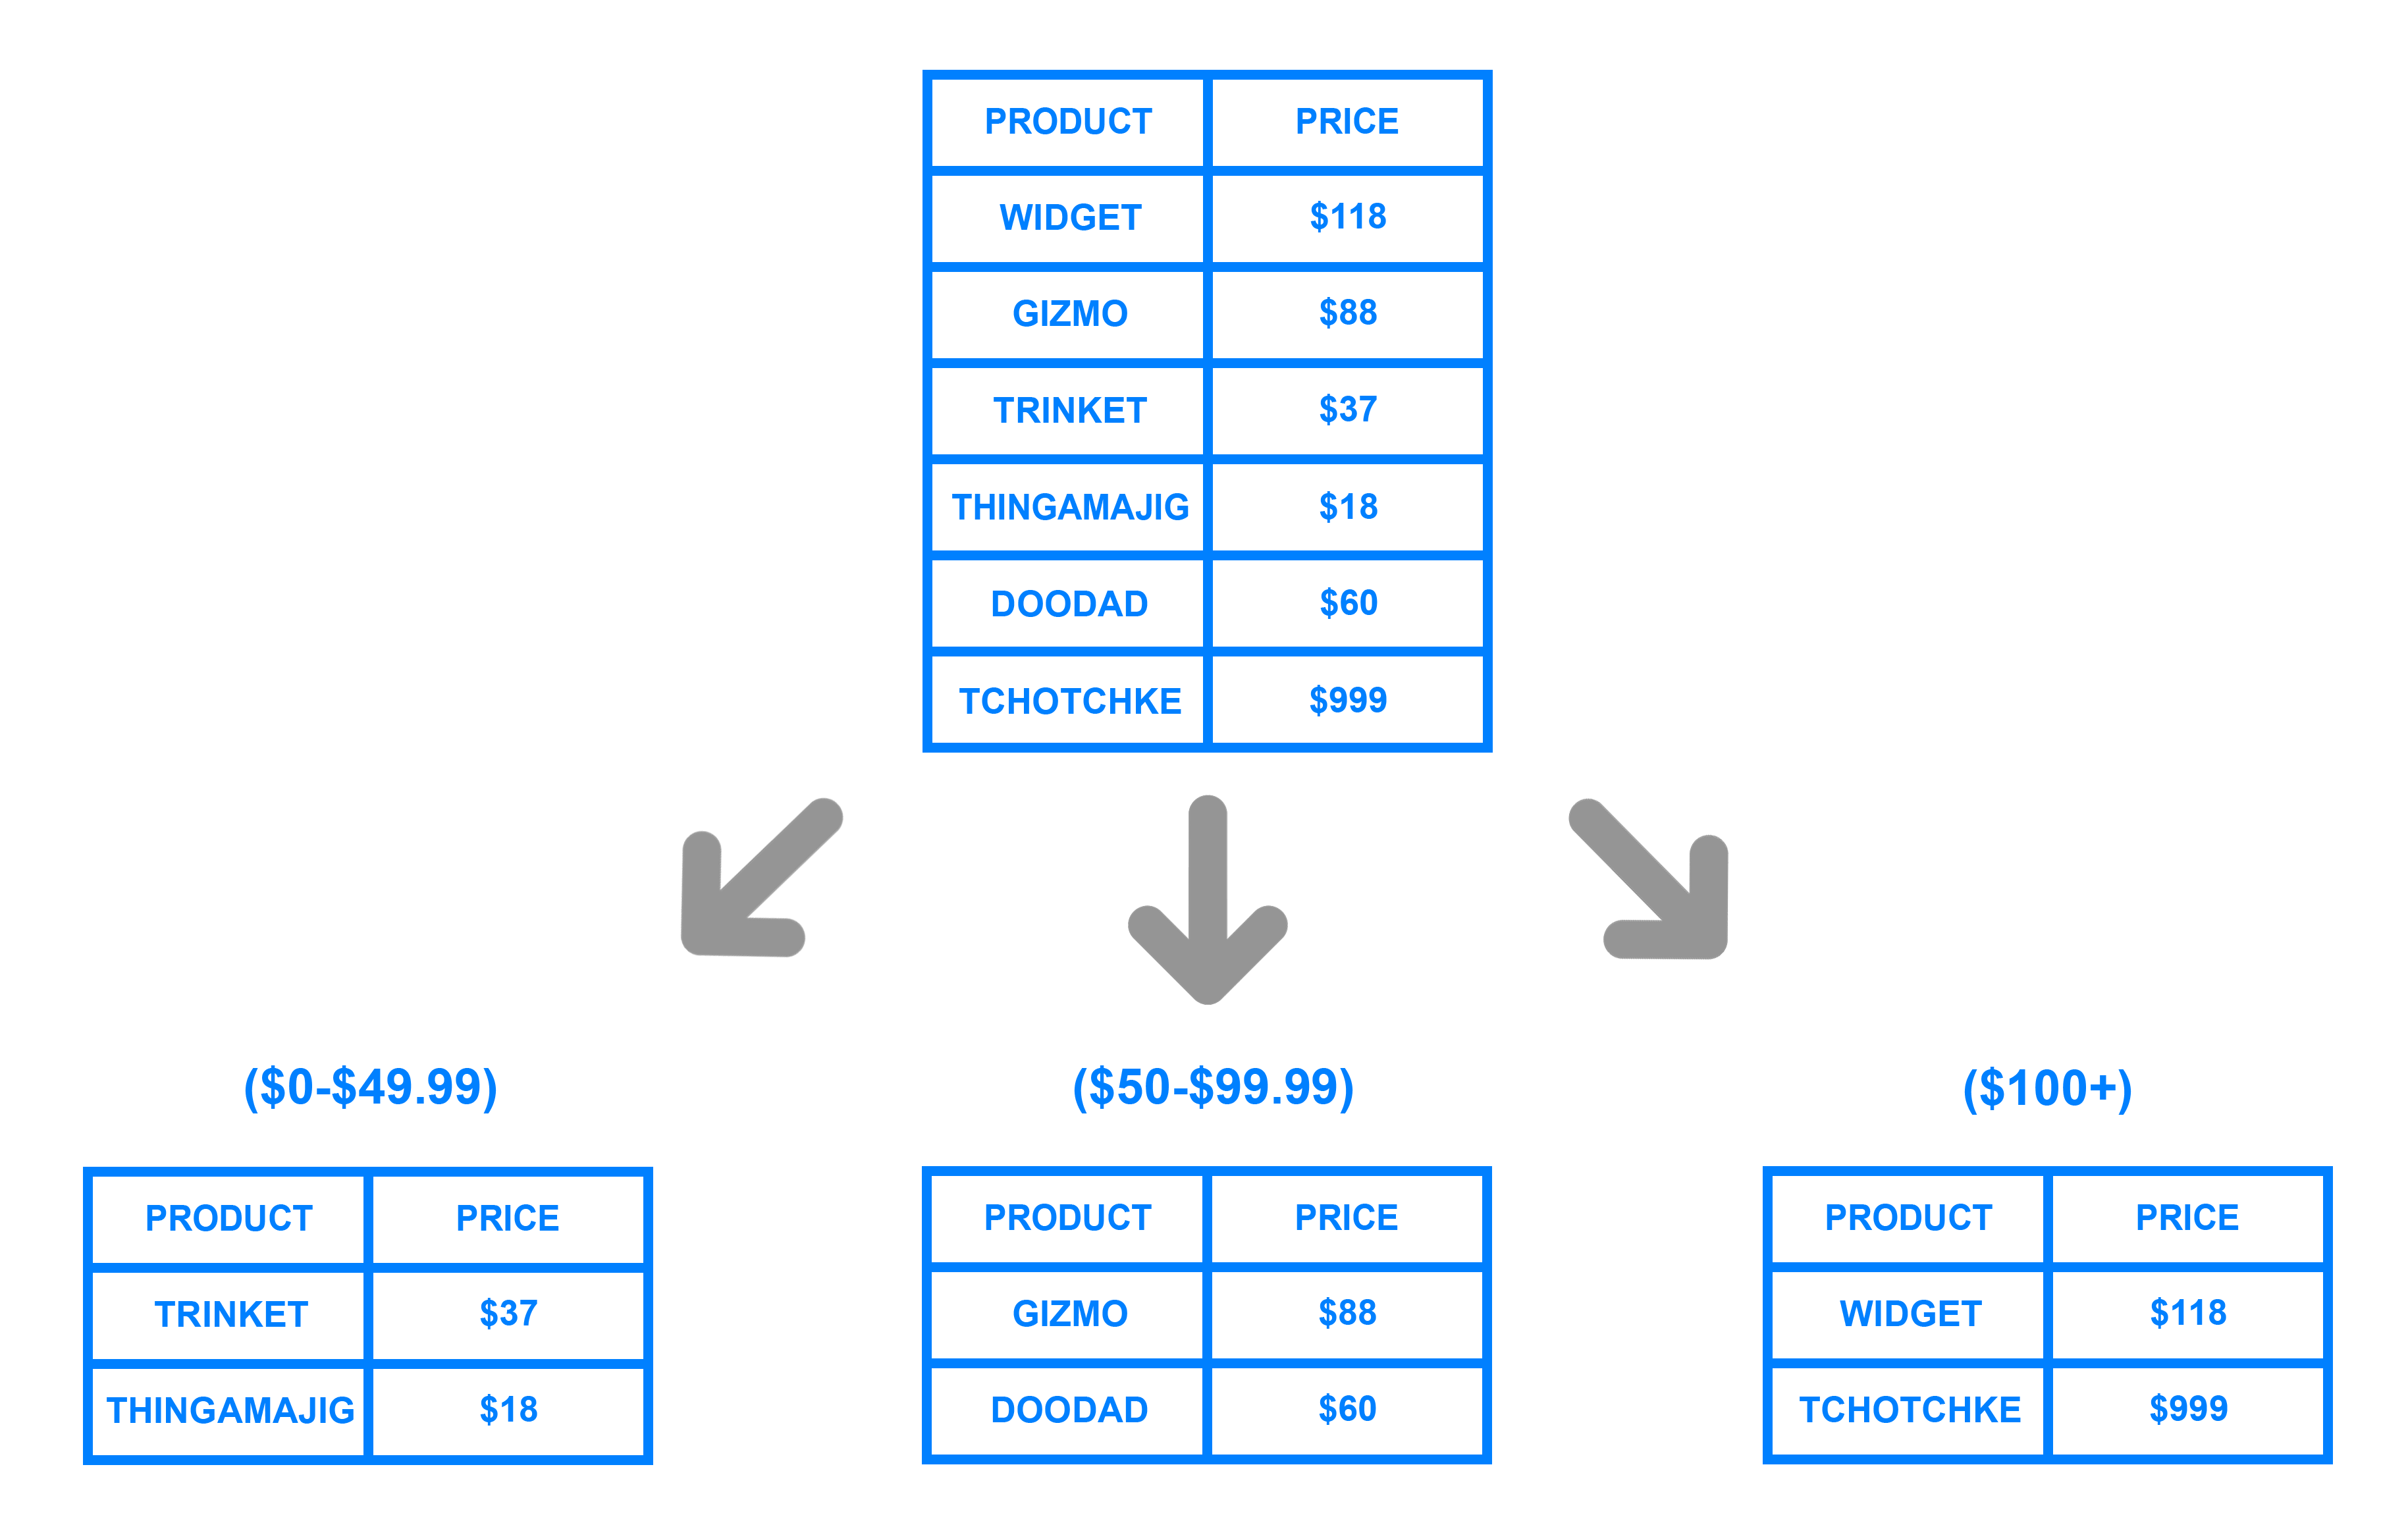
\includegraphics[width=100mm]{assets/distributed/Horizontal-Sharding}
    \caption{Горизонтальное шардирование}
    \label{fig:Horizontal-Sharding}
\end{figure}

\textbf{Горизонтальное шардирование} - самый простой метод сегментирования для реализации. Каждый осколок содержит
другой набор данных, но все они имеют ту же схему, что и исходная база данных. В этом методе вам просто нужно
определить, в какой диапазон попадают ваши данные, а затем вы можете сохранить запись в соответствующий шард. Этот
метод лучше всего подходит для хранения нестатических данных (например, хранение контактной информации студентов
колледжа).

Недостатком этого метода является то, что данные могут быть неравномерно распределены по шардам. В приведенном выше
примере у вас может быть много клиентов, имена которых попадают в категорию A-P. В таких случаях первый осколок должен
будет взять на себя больше нагрузки, чем второй, и это может стать узким местом системы. \autocite{DatabaseSharding}

\paragraph{Вертикальное шардирование} ~\\
В этом методе мы разделяем весь столбец из таблицы и помещаем эти столбцы в новые отдельные таблицы. Данные полностью
независимы от одного раздела к другому. Кроме того, каждый раздел содержит как отдельные строки, так и столбцы. Возьмем,
к примеру, функции Twitter. Мы можем разделить различные функции объекта на разные сегменты на разных машинах. В
Твиттере у пользователя может быть профиль, количество подписчиков и некоторые твиты, опубликованные им самим. Мы можем
разместить профили пользователей на одном осколке, подписчиков - на втором, а твиты - на третьем.

\begin{figure}[H]
    \centering
    \includegraphics[width=100mm]{assets/distributed/Vertical-Sharding}
    \caption{Вертикальное шардирование}
    \label{fig:Vertical-Sharding}
\end{figure}

В этом методе вы можете отделить и обработать критическую часть (например, профили пользователей) от некритической части
ваших данных (например, сообщения в блоге) по отдельности и построить вокруг нее различные модели репликации и
согласованности. Это одно из главных преимуществ этого метода.

Основным недостатком этой схемы является то, что для ответа на некоторые запросы вам, возможно, придется комбинировать
данные из разных шардов, что неоправданно увеличивает сложность разработки и эксплуатации системы. Кроме того, если
ваше приложение будет расти позже, и вы добавите в него еще несколько функций, вам придется дополнительно сегментировать
базу данных с конкретными функциями на нескольких серверах. \autocite{DatabaseSharding}

\paragraph{Шардинг на основе каталогов} ~\\
В этом методе мы создаем и поддерживаем службу поиска или таблицу поиска для исходной базы данных. В основном мы
используем ключ осколка для таблицы поиска и делаем сопоставление для каждого объекта, существующего в базе данных.
Таким образом, мы отслеживаем, какие осколки базы данных содержат какие данные.

Таблица поиска содержит статический набор информации о том, где можно найти конкретные данные. На приведенном выше
изображении вы можете видеть, что мы использовали зону доставки в качестве ключа осколка. Во-первых, клиентское
приложение запрашивает службу поиска, чтобы узнать осколок (раздел базы данных), на котором размещены данные. Когда
служба поиска возвращает осколок, она запрашивает/обновляет этот осколок.

\begin{figure}[H]
    \centering
    \includegraphics[width=100mm]{assets/distributed/Directory-Based-Sharding}
    \caption{Шардинг на основе каталогов}
    \label{fig:Directory-Based-Sharding}
\end{figure}

Сегментация на основе каталогов гораздо более гибкая, чем сегментация на основе диапазонов и ключей. В сегменте на
основе диапазонов вы обязаны указать диапазоны значений. В key-based вы обязаны использовать фиксированную хэш-функцию,
которую трудно изменить позже. При таком подходе вы можете использовать любой алгоритм, который хотите назначить для
записей данных в сегменты. Кроме того, при таком подходе легко динамически добавлять шарды.

Основным недостатком этого подхода является единственная точка отказа таблицы поиска. Если он будет поврежден или не
удался, это повлияет на запись новых данных или доступ к существующим данным из таблицы. \autocite{DatabaseSharding}

\paragraph{Шардинг на основе ключей} ~\\
Этот метод также известен как сегментация на основе хэша. Здесь мы берем значение объекта, такого как идентификатор
клиента, адрес электронной почты клиента, IP-адрес клиента, почтовый индекс и т. д., и мы используем это значение в
качестве входных данных хэш-функции. Этот процесс генерирует хэш-значение, которое используется для определения того,
какой шард нам нужно использовать для хранения данных. Мы должны иметь в виду, что значения, введенные в хэш-функцию,
должны поступать из одного и того же столбца (ключ осколка), чтобы данные размещались в правильном порядке и
согласованно. В принципе, ключи осколков действуют как первичный ключ или уникальный идентификатор для отдельных строк.

\begin{figure}[H]
    \centering
    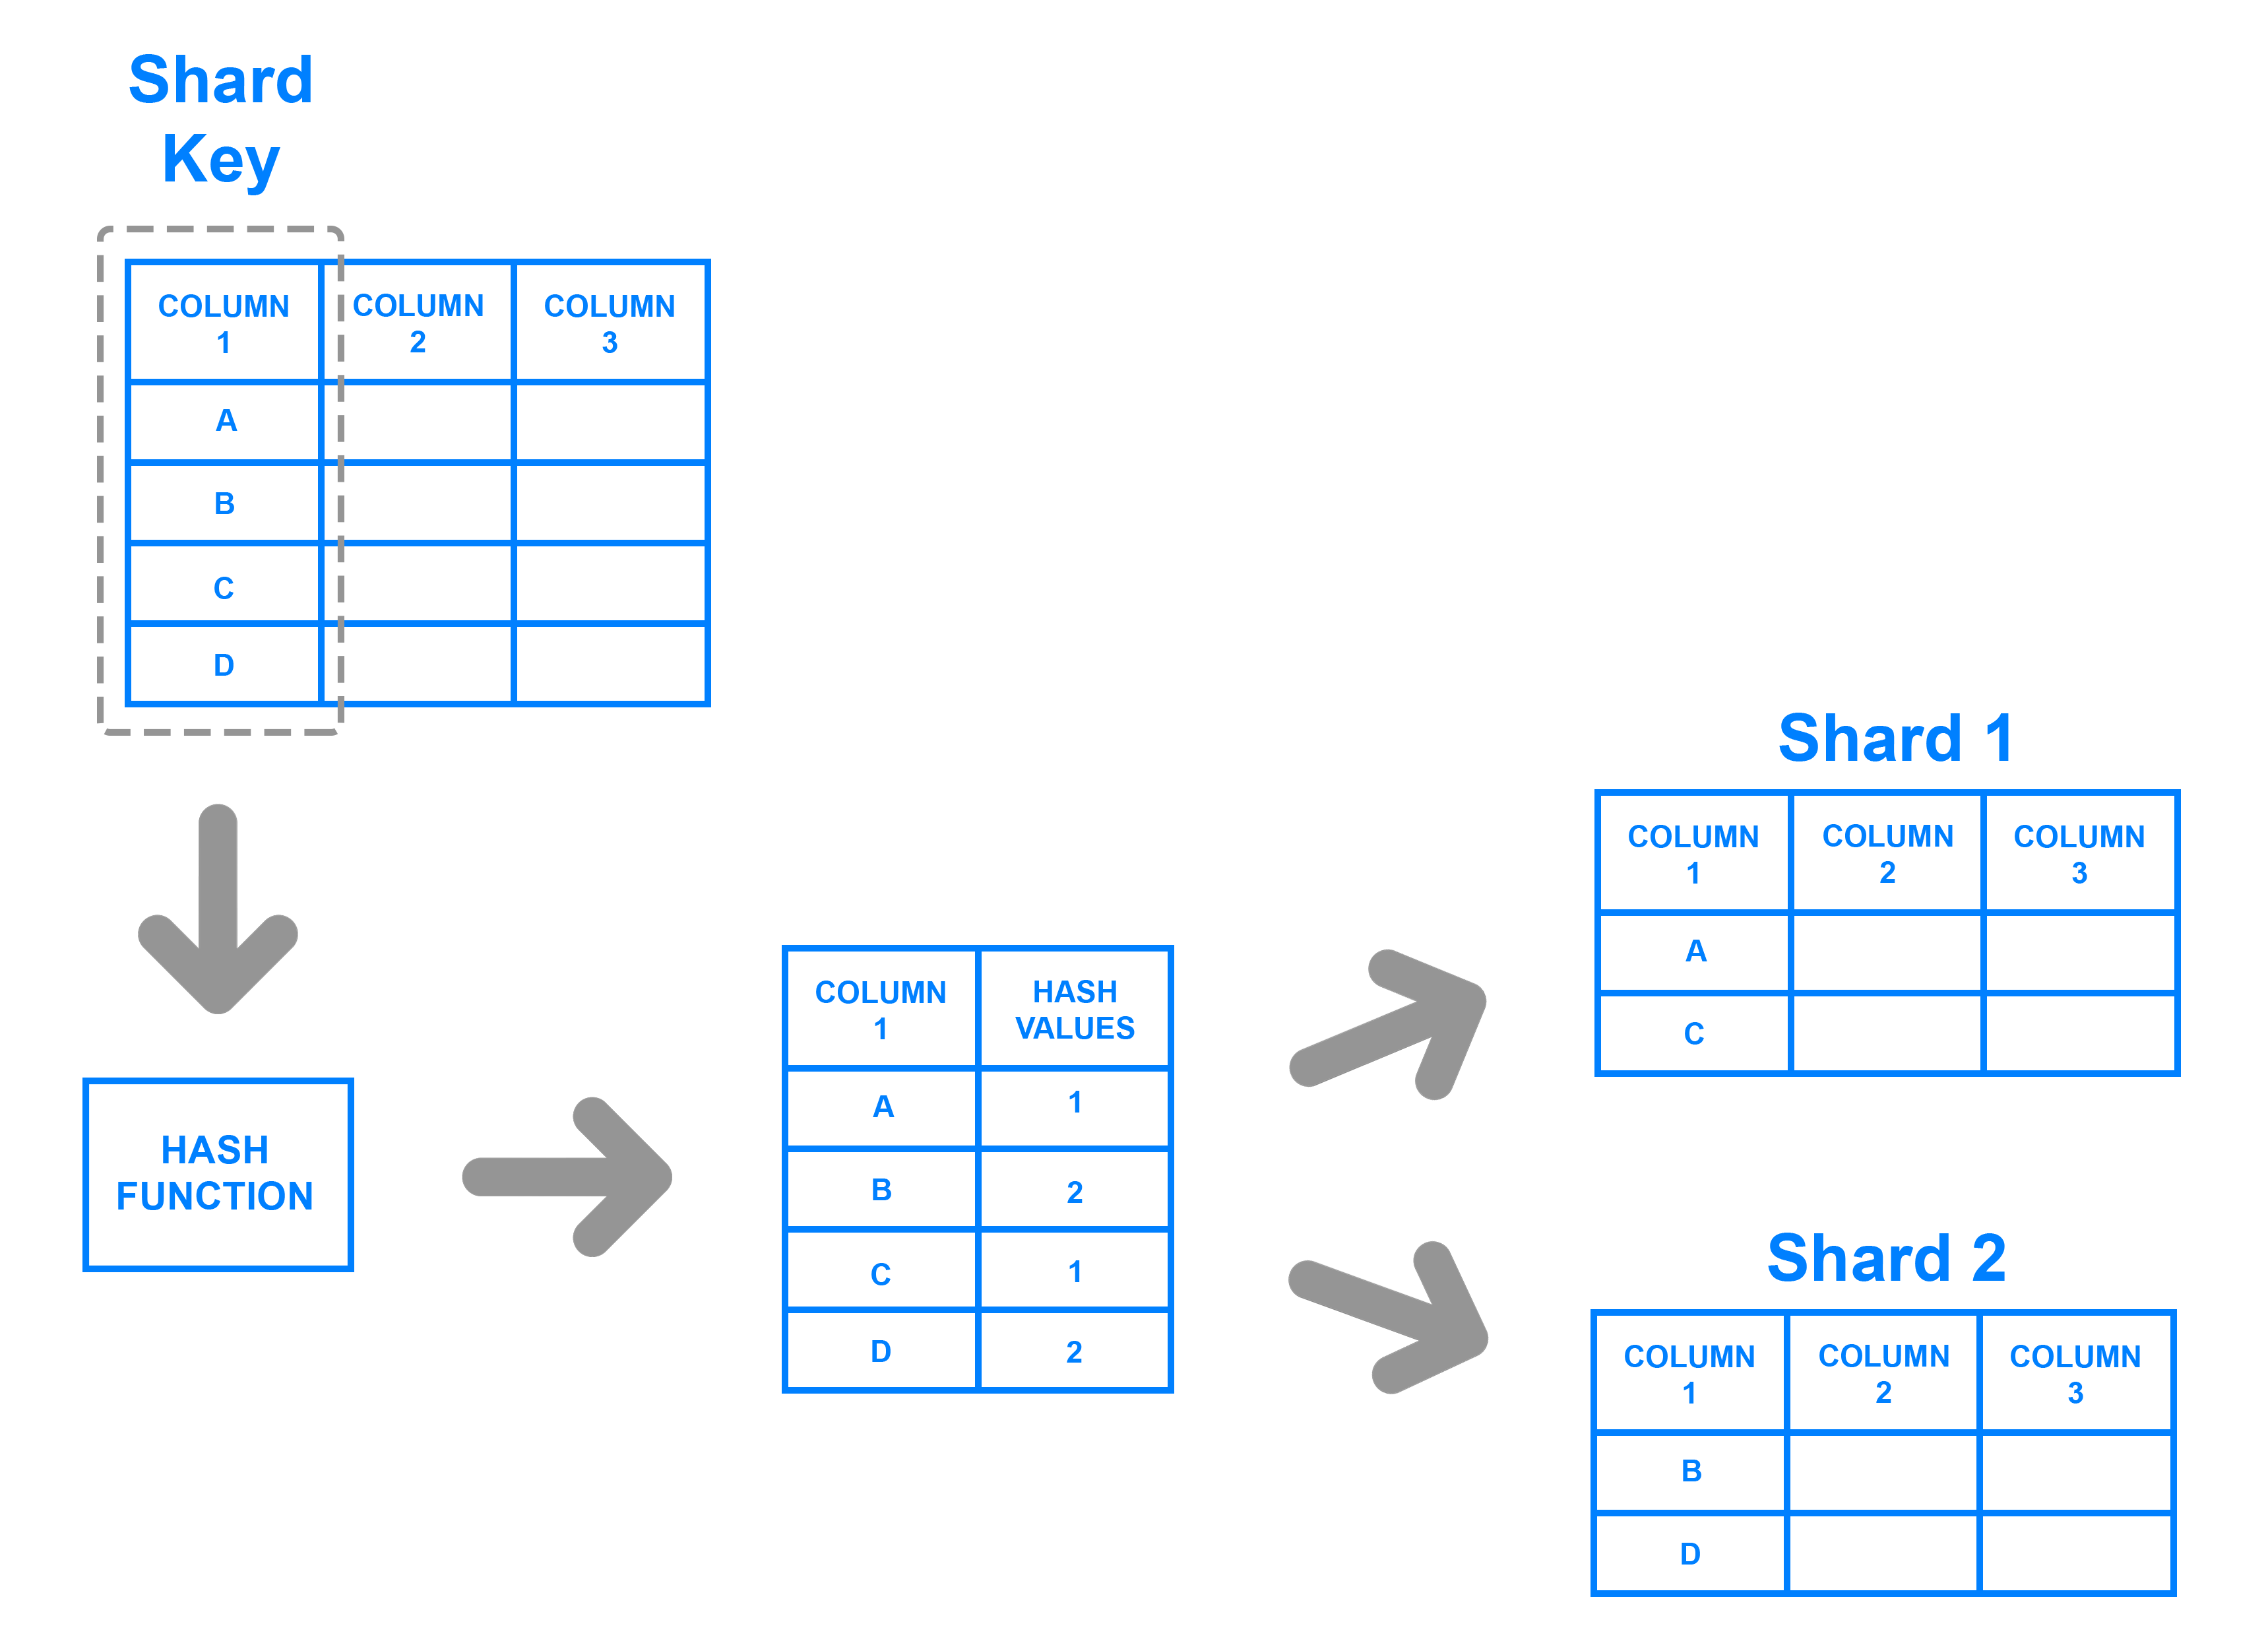
\includegraphics[width=100mm]{assets/distributed/Keybased-Sharding}
    \caption{Шардинг на основе ключей}
    \label{fig:Keybased-Sharding}
\end{figure}

Рассмотрим пример, что у вас есть 3 сервера баз данных, и каждый запрос имеет идентификатор приложения, который
увеличивается на 1 каждый раз, когда регистрируется новое приложение. Чтобы определить, на каком сервере должны быть
размещены данные, мы выполняем операцию по модулю для этих приложений id с номером 3. Затем остаток используется для
идентификации сервера для хранения наших данных.

Недостатком этого метода является эластичная балансировка нагрузки, что означает, если вы попытаетесь динамически
добавлять или удалять серверы баз данных, это будет сложный и дорогостоящий процесс. Например, в приведенном выше
примере, если вы добавите еще 5 серверов, вам нужно добавить больше соответствующих хэш-значений для дополнительных
записей. Кроме того, большинство существующих ключей необходимо переназначить на их новое, правильное хэш-значение,
а затем перенести на новый сервер. Хэш-функция должна быть изменена с модуля 3 на модуль 8. В то время как миграция
данных действует, как новые, так и старые хэш-функции не будут действительны. Во время миграции ваше приложение не
сможет обслуживать большое количество запросов, и вы будете испытывать простои для своего приложения до завершения
миграции. \autocite{DatabaseSharding}

\paragraph{Географический шардинг} ~\\
Шардирование по географическому признаку позволяет хранить определенные данные вблизи своих потребителей и
удовлетворять нормативным требованиям, когда данные должны находиться в определенной юрисдикции. Однако данный способ
шардирования не является самодостаточным: шарды могут быть загружены не равномерно, и отличие может быть на порядки.
На пример, экземпляр базы данных, хранящий данные пользователей Москвы и Московской области, будет намного превышать
другой экземпляр базы данных, который хранит информацию о пользователях из Владимира. Таким образом, недостатком
данного метода является необходимость дополнительного использования других методов шардирования.

\paragraph{Репликация} ~\\
\textbf{Репликация} — это процесс изменения одного набора данных, называемого репликой, в ответ на изменения другого
набора данных, называемого основным. Репликация желательна по крайней мере по двум причинам. Во-первых, она способна
обеспечить более высокую производительность, поскольку приложения смогут обрабатывать локальные копии вместо того,
чтобы устанавливать связь с удаленными узлами. Во-вторых, наличие репликации может также обеспечивать более высокую
степень доступности, поскольку любой реплицируемый объект остается доступным для обработки (по крайней мере, для выборки
данных), пока хотя бы одна реплика в системе остается доступной. Главным недостатком репликации, безусловно, является
то, что если реплицируемый объект обновляется, то и все его копии должны быть обновлены (проблема распространения
обновлений).

Очевидно, что репликация, как и шардирование, теоретически должна быть "прозрачной для пользователя". Другими словами,
система, которая поддерживает репликацию данных, должна также поддерживать независимость от репликации (иногда говорят
"прозрачность репликации"). Для пользователей должна быть создана такая среда, чтобы они, по крайней мере, с логической
точки зрения могли считать, что в действительности данные не дублируются. Независимость от репликации (как и
независимость от шардирования) является весьма желательной, поскольку она упрощает создание пользовательских программ и
выполнение терминальных операций. В частности, независимость от репликации позволяет создавать и уничтожать дубликаты в
любой момент в соответствии с изменяющимися требованиями, не затрагивая при этом никакие из пользовательских программ
или терминальных операций.

Из требования независимости от репликации следует, что к обязанностям системного оптимизатора также относится
определение, какой именно из физических дубликатов будет применен для доступа к данным при выполнении каждого
введенного пользователем запроса. \autocite{IntroBD2014}

Можно выделить три \textbf{подхода к репликации}:
\begin{itemize}
    \item Блочная репликация на уровне системы хранения данных;
    \item Физическая репликация на уровне СУБД;
    \item Логическая репликация на уровне СУБД.
\end{itemize}

\paragraph{Блочная репликация} ~\\
При блочной репликации каждая операция записи выполняется не только на основном диске, но и на резервном. Таким образом
тому на одном массиве соответствует зеркальный том на другом массиве, с точностью до байта повторяющий основной том.

К достоинствам такой репликации можно отнести простоту настройки и надёжность. Записывать данные на удалённый диск может
либо дисковый массив, либо нечто (устройство или программное обеспечение), стоящее между хостом и диском. Если дисковый
массив не способен реплицировать данные, между хостом и массивом может быть установлен агент, осуществляющей запись на
два массива сразу. Агент может быть как отдельным устройством, так и программным компонентом. В отличие от дискового
массива, который может работать только с таким же массивом или, как минимум, с массивом того же производителя, агент
может работать с совершенно разными дисковыми устройствами.

Главное назначение блочной репликации – обеспечение отказоустойчивости. Если база данных потеряна, то можно
перезапустить её с использованием зеркального тома. Блочная репликация хороша своей универсальностью, но за
универсальность приходится платить.

Во-первых, никакой сервер не может работать с зеркальным томом, поскольку его операционная система не может управлять
записью на него; с точки зрения наблюдателя данные на зеркальном томе появляются сами собой. В случае аварии (отказ
основного сервера или всего ЦОДа, где находится основной сервер) следует остановить репликацию, размонтировать основной
том и смонтировать зеркальный том. Как только появится возможность, следует перезапустить репликацию в обратном
направлении.

Во-вторых, сама СУБД на резервном сервере может быть запущена только после монтирования диска. В некоторых операционных
системах, например, в Solaris, память под кеш при выделении размечается, и время разметки пропорционально объёму
выделяемой памяти, то есть старт экземпляра будет отнюдь не мгновенным. Плюс ко всему кеш после рестарта будет пуст.

В-третьих, после запуска на резервном сервере СУБД обнаружит, что данные на диске неконсистентны, и нужно потратить
значительное время на восстановление с применением журналов повторного выполнения: сначала повторить те транзакции,
результаты которых сохранились в журнале, но не успели сохраниться в файлы данных, а потом откатить транзакции, которые
к моменту сбоя не успели завершиться. \autocite{Replication}

\paragraph{Физическая репликация (master-slave)} ~\\
Журналы (redo log или write-ahead log) содержат все изменения, которые вносятся в файлы базы данных. Идея физической
репликации состоит в том, что изменения из журналов повторно выполняются в другой базе (реплике), и таким образом данные
в реплике повторяют данные в основной базе байт-в-байт.

Журналы СУБД не предназначены для использования вне этой платформы, их формат не документируется и может меняться без
предупреждения. Отсюда совершенно естественное требование, что физическая репликация возможна только между экземплярами
одной и той же версии одной той же СУБД. Отсюда же возможные ограничения на операционную систему и архитектуру
процессора, которые тоже могут влиять на формат журнала.

Естественно, никаких ограничений на модели СХД физическая репликация не накладывает. Более того, файлы в базе-реплике
могут располагаться совсем по-другому, чем на базе-источнике – надо лишь описать соответствие между томами, на которых
лежат эти файлы.

Запись данных в реплику невозможна, поскольку изменения в неё приходят побайтно, и реплика не может обеспечить
конкурентное исполнение своих запросов. В случае повреждения файла в основной базе можно просто скопировать
соответствующий файл с реплики. Однако стоит учесть, что файл на реплике может быть не идентичен файлу в основной базе:
когда файл расширяется, новые блоки в целях ускорения ничем не заполняются, и их содержимое случайно. База может
использовать не всё пространство блока (например, в блоке может оставаться свободное место), но содержимое
использованного пространства совпадает с точностью до байта.

Физическая репликация может быть как синхронной, так и асинхронной. При асинхронной репликации всегда есть некий набор
транзакций, которые завершены на основной базе, но ещё не дошли до резервной, и в случае перехода на резервную базу при
сбое основной эти транзакции будут потеряны. При синхронной репликации завершение операции commit означает, что все
журнальные записи, относящиеся к данной транзакции, переданы на реплику. Важно понимать, что получение репликой журнала
не означает применения изменений к данным. При потере основной базы транзакции не будут потеряны, но если приложение
пишет данные в основную базу и считывает их из реплики, то у него есть шанс получить старую версию этих данных.

Физическая репликация базы данных имеет множество преимуществ перед репликацией средствами СХД:
\begin{itemize}
    \item объём передаваемых данных меньше за счёт того, что передаются только журналы, но не файлы с данными; эксперименты показывают уменьшение трафика в 5-7 раз;
    \item переключение на резервную базу происходит значительно быстрее: экземпляр-реплика уже поднят, поэтому при переключении ему нужно лишь откатить активные транзакции; более того, к моменту сбоя кеш реплики уже прогрет;
    \item на реплике можно выполнять запросы, сняв тем самым часть нагрузки с основной базы. В частности, реплику можно использовать для создания резервных копий.
\end{itemize}

\paragraph{Логическая репликация (active-active)} ~\\
Все изменения в базе данных происходят в результате вызовов её API – например, в результате выполнения SQL-запросов.
Очень заманчивой кажется идея выполнять одну и ту же последовательность запросов на двух разных базах. Для репликации
необходимо придерживаться двух правил:
\begin{itemize}
    \item нельзя начинать транзакцию, пока не завершены все транзакции, которые должны закончиться раньше; Так на рисунке ниже нельзя запускать транзакцию D, пока не завершены транзакции A и B;
    \item нельзя завершать транзакцию, пока не начаты все транзакции, которые должны закончиться до завершения текущей транзакции; Так на рисунке ниже даже если транзакция B выполнилась мгновенно, завершить её можно только после того, как начнётся транзакция C.
\end{itemize}

\begin{figure}[H]
    \centering
    \includegraphics[width=100mm]{assets/distributed/ReplicationExample}
    \caption{Пример репликации}
    \label{fig:ReplicationExample}
\end{figure}

\textbf{Репликация команд (statement-based replication)} реализована, например, в MySQL. К сожалению, эта простая схема не
приводит к появлению идентичных наборов данных – тому есть две причины.
\begin{itemize}
    \item не все API детерминированы. Например, если в SQL-запросе встречается функция now() или sysdate(), возвращающая текущее время, то на разных серверах она вернёт разный результат – из-за того, что запросы выполняются не одновременно. Кроме того, к различиям могут привести разные состояния триггеров и хранимых функций, разные национальные настройки, влияющие на порядок сортировки, и многое другое.
    \item репликацию, основанную на параллельном исполнении команд, невозможно корректно приостановить и перезапустить. На рисунке выше если репликация остановлена в момент T1 транзакция B должна быть прервана и откачена. При перезапуске репликации исполнение транзакции B может привести реплику к состоянию, отличному от состояния базы-источника: на источнике транзакция B началась до того, как закончилась транзакция A, а значит, она не видела изменений, сделанных транзакцией A. Репликация запросов может быть остановлена и перезапущена только в момент T2, когда в базе нет ни одной активной транзакции. Разумеется, на сколько-нибудь нагруженной промышленной базе таких моментов не бывает.
\end{itemize}

Обычно для логической репликации используют детерминированные запросы. Детерминированность запроса обеспечивается двумя
свойствами:
\begin{itemize}
    \item запрос обновляет (или вставляет, или удаляет) единственную запись, идентифицируя её по первичному (или уникальному) ключу;
    \item все параметры запроса явно заданы в самом запросе.
\end{itemize}

В отличие от \textbf{репликации команд (statement-based replication)} такой подход называется \textbf{репликацией
записей (row-based replication)}.

База-реплика открыта и доступна не только на чтение, но и на запись. Это позволяет использовать реплику для выполнения
части запросов, в том числе для построения отчётов, требующих создания дополнительных таблиц или индексов. Важно
понимать, что логическая реплика будет эквивалентна исходной базе только в том случае, если в неё не вносится никаких
дополнительных изменений

Логическая репликация предоставляет ряд возможностей, отсутствующих в других видах репликации:
\begin{itemize}
    \item настройка набора реплицируемых данных на уровне таблиц (при физической репликации – на уровне файлов и табличных пространств, при блочной репликации – на уровне томов);
    \item построение сложных топологий репликации – например, консолидация нескольких баз в одной или двунаправленная репликация;
    \item уменьшение объёма передаваемых данных;
    \item репликация между разными версиями СУБД или даже между СУБД разных производителей;
    \item обработка данных при репликации, в том числе изменение структуры, обогащение, сохранение истории.
\end{itemize}

Есть и недостатки, которые не позволяют логической репликации вытеснить физическую:
\begin{itemize}
    \item все реплицируемые данные обязаны иметь первичные ключи;
    \item логическая репликация поддерживает не все типы данных;
    \item логическая репликация на практике не бывает полностью синхронной: время от получения изменений до их применения слишком велико, чтобы основная база могла ждать;
    \item логическая репликация создаёт большую нагрузку на реплику;
    \item при переключении приложение должно иметь возможность убедиться, что все изменения с основной базы, применены на реплике – СУБД зачастую сама не может этого определить, так как для неё режимы реплики и основной базы эквивалентны.
\end{itemize}

Два последних недостатка существенно ограничивают использование логической реплики как средства отказоустойчивости. Если
один запрос в основной базе изменяет сразу много строк, реплика может существенно отставать. А возможность смены ролей
требует недюжинных усилий как со стороны разработчиков, так и со стороны администраторов.

Есть несколько способов реализации логической репликации, и каждый из этих способов реализует одну часть возможностей и
не реализует другую:
\begin{itemize}
    \item репликация триггерами;
    \item использование журналов СУБД;
    \item использование программного обеспечения класса CDC (change data capture);
    \item прикладная репликация.
\end{itemize}

\paragraph{Репликация триггерами} ~\\
Триггер – хранимая процедура, которая исполняется автоматически при каком-либо действии по модификации данных. Триггеру,
который вызывается при изменении каждой записи, доступны ключ этой записи, а также старые и новые значения полей. При
необходимости триггер может сохранять новые значения строк в специальную таблицу, откуда специальный процесс на стороне
реплики будет их вычитывать

\textbf{Преимущества}:
\begin{itemize}
    \item независимость от версий основной базы и реплики;
    \item широкие возможности преобразования данных.
\end{itemize}

\textbf{Недостатки}:
\begin{itemize}
    \item нагрузка на основную базу;
    \item большая задержка при репликации.
\end{itemize}

\paragraph{Использование журналов СУБД} ~\\
Сами СУБД также могут предоставлять возможности логической репликации. Источником данных, как и для физической
репликации, являются журналы. К информации о побайтовом изменении добавляется также информация об изменённых полях, а
также значение уникального ключа, даже если он не меняется. В результате объём журналов БД увеличивается – по разным
оценкам от 10 до 15%.

К \textbf{недостаткам} данного подхода можно отнести увеличение объёма журналов и возможное увеличение трафика между
узлами.

\paragraph{Использование CDC} ~\\
Существует целый класс программного обеспечения, предназначенного для организации логической репликации. Это ПО
называется CDC, change data capture. В задачу платформы входит чтение журналов базы данных, преобразование информации,
передача информации на реплику и применение. Как и в случае репликации средствами самой СУБД, журнал должен содержать
информацию об изменённых полях. Использование дополнительного приложения позволяет «на лету» выполнять сложные
преобразования реплицируемых данных и строить достаточно сложные топологии репликации.

\textbf{Преимущества}:
\begin{itemize}
    \item возможность репликации между разными СУБД, в том числе загрузка данных в отчётные системы;
    \item широчайшие возможности обработки и преобразования данных;
    \item минимальный трафик между узлами – платформа отсекает ненужные данные и может сжимать трафик;
    \item встроенные возможности мониторинга состояния репликации.
\end{itemize}

\textbf{Недостатки}:
\begin{itemize}
    \item увеличение объёма журналов, как при логической репликации средствами СУБД;
    \item новое ПО – сложное в настройке и/или с дорогими лицензиями.
\end{itemize}

\paragraph{Прикладная репликация} ~\\
Наконец, ещё один способ репликации – формирование векторов изменений непосредственно на стороне клиента. Клиент должен
формировать детерминированные запросы, затрагивающие единственную запись. Добиться этого можно, используя специальную
библиотеку работы с базой данных. Когда приложение завершает транзакцию, специально подключаемый модуль записывает
вектор изменений в очередь и выполняет транзакцию в базе данных. Специальный процесс-репликатор вычитывает векторы из
очереди и выполняет транзакции в базе-реплике.Этот механизм хорош для обновления отчётных систем. Может он
использоваться и для обеспечения отказоустойчивости, но в этом случае в приложении должен быть реализован контроль
состояния репликации

\textbf{Преимущества}:
\begin{itemize}
    \item возможность репликации между разными СУБД, в том числе загрузка данных в отчётные системы;
    \item возможность обработки и преобразования данных, мониторинга состояния и т. д.;
    \item минимальный трафик между узлами – платформа отсекает ненужные данные и может сжимать трафик;
    \item полная независимость от базы данных – как от формата, так и от внутренних механизмов.
\end{itemize}

\textbf{Недостатки}:
\begin{itemize}
    \item ограничения на архитектуру приложения;
    \item огромный объём собственного кода, обеспечивающего репликацию.
\end{itemize}

\paragraph{Сравнение подходов к репликации} ~\\
Описав все подходы к репликации, можно установить следующее:
\begin{itemize}
    \item \textbf{Блочная репликация} имеет смысл, когда других способов репликации нет; для баз данных её лучше не использовать.
    \item \textbf{Физическая репликация} хороша, когда требуется обеспечение отказоустойчивости инфраструктуры или перенос части читающих приложений на реплики.
    \item \textbf{Логическая репликация} подходит для обеспечения отказоустойчивости только в том случае, если приложение знает об этой репликации и умеет в случае аварии ждать синхронизации реплик.
    \item \textbf{Логическая репликация} идеальна для всевозможных отчётных баз.
    \item \textbf{Репликация триггерами} имеет смысл в том случае, если база сильно нагружена, а реплицировать нужно крайне ограниченное количество информации.
    \item \textbf{Платформы CDC} хороши, если у вас большое количество реплицируемых баз и/или есть необходимость сложных преобразований данных.
    \item Разработка \textbf{прикладной репликации} оправдана только в случае разработки собственной платформы или фреймворка.
\end{itemize} \autocite{Replication}

\paragraph{Greenplum} ~\\
Ранее уже сравнивались различные подходы шардирования между собой. Сравнивались различные подходы репликации между
собой. Осталось только сравнить способы тиражирования, то есть сравнить репликацию и шардирование.

Вообще говоря, шардинг и репликация не противоречат друг другу и могут сосуществовать. Они выполняют разные задачи, и
сравнивать их не имеет смысла. Репликация используется для ускорения взаимодействия с бд с помощью использования копий
основной базы данных. Кроме того, репликация осуществляет отказоустойчивость. В свою очередь шардинг осуществляет
ускорение работы с базой данных с помощью разбиения исходной базы данных на несколько разных, хранящихся на разных
серверах.  Шардирование не реализует отказоустойчивость.

В принципе, на этом их сравнение можно закончить и перейти к примеру. Один из классических примеров в котором
реализовано сочетание репликации и шардирования - \textbf{Greenplum}.

\textbf{Greenplum (GP)} – реляционная СУБД, имеющая массово-параллельную (massive parallel processing) архитектуру без
разделения ресурсов (Shared Nothing). В общем случае кластер GP состоит из нескольких серверов-сегментов (именно
сегменты непосредственно хранят данные, выполняют с ними операции и отдают результаты мастеру (в общем случае). По сути
сегмент – самый обычный инстанс PostgreSQL 8.2.15 с настроенной логической репликацией в своё зеркало на другом
сервере), одного сервера-мастера (сервер, на котором работает инстанс, являющийся одновременно координатором и входной
точкой для пользователей в кластере), и одного сервера-секондари-мастера (инстанс, являющийся резервным мастером,
включается в работу в случае недоступности основного мастера (переключение происходит вручную)), соединённых между
собой одной или несколькими быстрыми (10g, infiniband) сетями, обычно обособленными (interconnect). На рисунке ниже
представлен состав кластера и сетевое взаимодействие элементов. Здесь — зелёная и красная линии — обособленные сети
interconnect, синяя линия — внешняя, клиентская сеть.

\begin{figure}[H]
    \centering
    \includegraphics[width=100mm]{assets/distributed/Greenplum}
    \caption{Состав кластера и сетевое взаимодействие элементов Greenplum}
    \label{fig:Greenplum}
\end{figure}

При выборе числа серверов-сегментов важно правильно выбрать соотношение кластера «число процессоров/Тб данных» в
зависимости от планируемого профиля нагрузки на БД — чем больше процессорных ядер приходится на единицу данных, тем
быстрее кластер будет выполнять «тяжёлые» операции, а также работать со сжатыми таблицами.

При выборе числа сегментов в кластере (которое в общем случае к числу серверов никак не привязано) необходимо помнить
следующее:
\begin{itemize}
    \item все ресурсы сервера делятся между всеми сегментами на сервере (нагрузкой зеркал, в случае если они располагаются на этих же серверах, можно условно пренебречь);
    \item каждый запрос на одном сегменте не может потреблять процессорных ресурсов больше, чем одно ядро CPU. Это означает, например, что, если кластер состоит из 32-ядерных серверов с 4-я сегментами GP на борту и используется в среднем для обработки 3-4 одновременных тяжёлых, хорошо утилизирующих CPU, запросов, «в среднем по больнице» CPU не будет утилизироваться оптимально. В данной ситуации лучше увеличить число сегментов на сервере до 6-8;
    \item штатный процесс бекапа и рестора данных «из коробки» работает только на кластерах, имеющих одинаковое число сегментов. Восстановить данные, забекапленные на кластере из 96 сегментов, в кластер из 100 сегментов без напильника будет невозможно.
\end{itemize}

В Greenplum реализуется классическая схема шардирования данных. Каждая таблица представляет из себя N+1 таблиц на всех
сегментах кластера, где N – число сегментов (+1 в этом случае — это таблица на мастере, данных в ней нет). На каждом
сегменте хранится 1/N строк таблицы. Логика разбиения таблицы на сегменты задаётся ключом (полем) дистрибуции – таким
полем, на основе данных которого любую строку можно отнести к одному из сегментов.

По подробнее почитать про Greenplum можно в источнике. В данной главе приведена только краткая информация об общей
архитектуре и информация, относящаяся к тиражированию данных. \autocite{Greenplum}

\subsection{Бесконфликтные реплицированные типы данных}
\paragraph{Проблема репликации}
Предположим, реплики СУБД распределены по географическому признаку для ускорения работы приложения. А теперь пусть в разных репликах практически одновременно и независимо была изменена одна и та же строка. Какую строку считать правильно отражающей данные? Как восстановить согласованность между репликами? В общем случае, проблема одновременного обновления реплик не может быть разрешима. Поэтому большинство распределенных СУБД запрещают производить такие операции, например используя только один сервер для выполнения запросов. Однако существует некоторый класс структур данных, которые позволяют автоматически разрешать конфликты возникающие в процессе обновления нескольких реплик. Этот класс называется - бесконфликтные реплицированные типы данных или conflict-free replicated data types(CRDT). 
\paragraph{CRDT. Опеределение и виды}
CRDT обладают следующими характеристиками:
\begin{itemize}
    \item Приложение может обновлять реплики независимо, параллельно с другими репликами
    \item Алгоритм(как часть CRDT) автоматически разрешает возможные конфликты
    \item Данные в разных репликах могут быть в различных состояниях в один и тот же момент времени, но они гарантированно сойдутся спустя некоторое время 
\end{itemize}
Просто используя специализированные структуры данных было бы сложно добиться бесконфликтности, поэтому для ее достижения используются также специальные алгоритмы обновления данных. Алгоритмы определяют требования к структурам данных, а также могут накладывать дополнительные требования на сети передачи данных. Рассмотрим два основных вида алгоритмов:
\begin{itemize}
    \item Operation-based CRDTs. При обновлении данных, на реплике генерируется специальная функция обновления, которая затем рассылается всем другим нодам в сети. Каждая нода применяет эту функцию к своим данным и таким образом достигается консистентность. Важно, чтобы каждая функция была лишь раз применена на каждой ноде. Поэтому необходимо следить за тем, чтобы доставка гарантированно произошла и произошла только один раз. Связано это с тем, что функции могут быть коммутативными, но далеко не факт, что они будут идемпотентными(применение несколько раз подряд дает разные результаты).
    \item State-based CRDTs. При обновлении данных, репликам посылается полная локальная копия данных, после чего реплики локально у себя сливают эти изменения воедино, причем операция слияния (merge) обладает свойствами ассоциативности, коммутативности и идемпотентности, что позволяет уменьшить требования к каналам связи между репликами. 
    \item Delta-state CRDTs - оптимизированный вариант state-based CRDTs, когда посылаются только недавно примененные изменения вместо полной копии состояния.
\end{itemize}
Помимо алгоритмов, важную роль играют процессы сходимости между нодами. Для сходимости в случае Operation-based CRDTs, каждая нода обязана получить ровно одно сообщение с фукнцией обновления и для этого необходим надежный протокол доставки. В случае с State-base CRDTs, наличие коммутативного и идемпотентного оператора слияния позволяет утверждать, что данные постепенно сойдутся в любом случае, что дает нам право не беспокоиться о протоколе доставки. 
\paragraph{Примеры реализации}
На сегодняшний день известных CRDT не так много, одни из них: G-Counter (Grow only counter), PN-Counter (positive-negative counter), G-Set (grow only set) и несколько других типов. Основной особенностью всех этих типов данных является, то что каждая коллекция поддерживает узкий набор операций. А чтобы добавить например вычитание (некоммутативную операцию) в PN-Counter необходимо прибегать к хитрости и использовать два ворастающих счетчика типа G-Counter. Рассмотрим пример реалиции G-Counter-а. 
\begin{figure}[H]
    \centering
    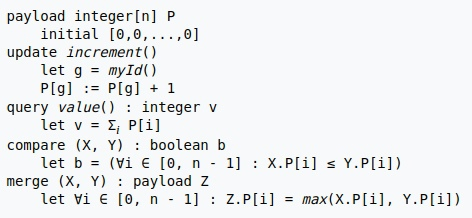
\includegraphics[width=100mm]{assets/distributed/G-Counter}
    \caption{Пример реализации Grow only Counter-а}
    \label{fig:G-Counter}
\end{figure}
Этот State-based счетчик сделан для кластера из n нод. Каждой ноде присвоен id, который можно получить вызвав функцию myid(). Таким образом, каждой ноде присваивается свой слот в массиве P, который нода может инкрементировать локально. Обновления расходятся по сети и при слиянии вычисляется максимум для каждого слота. При запросе значения счетчика все значения в слотах вектора суммируются и возвращаются в качестве ответа. Функция слияния является идемпотентной и коммутативной, поэтому данный счетчик является state-based.
Использование CRDT позволяет существенно упростить жизнь для разработчиков СУБД и облегчить работу с репликами. Уже сейчас CRDT используется во многих крупных проектах. В их число входит: Redis, Riak, Apple, Facebook. В дальнейшем использование CRDT будет только увеличиваться. 

\subsection{Интеграция БД и Internet}
\paragraph{Современные тенденции}
Заключаются в том, чтоб забыть о физических машинках и виртуалках, завернуть сервисы в контейнеры и перенести их в облако.

\paragraph{Обзор существующих технологий}
То немногое, из чего действительно полезно почитать хотя бы описание инструментов по диагонали.

\subparagraph{Docker} ~\\

    Docker~--- средство виртуализации и менеджмента программ (сервисов), позволяющее гибко настраивать инфраструктуру проектов, и кратно облегчающее разработку, тестирование и масштабируемый деплой.
    Архитектура у Docker клиент-серверная, что означает наличие демона dockerd и клиентов docker, отправляющих демону команды (собери, скачай, запусти, пр.). Если вам нужно на коленке запустить оркестрацию
    (операции ``возьми n нод, запусти на них k заданий (образов Docker) и проследи, чтоб выполнились''), можно использовать docker swarm. \autocite{DockerSwarmConcepts} В проде такое лучше не использовать,
    потому что ноды приходится создавать ручками; иными словами, если у вас есть 2 машинки с разным количеством ресурсов каждая, придётся собственными силами подстраивать количество запускаемых на машинке нод,
    подстраиваясь под потребляемые ресурсы. Если требуется динамическое масштабирование, лучше посмотреть в сторону K8s.

    \textbf{Контейнеры} ~\\
    Основная идея~--- завернуть необходимый сервис (бинарники, скрипты, данные, конфиги) в легковесный \textbf{контейнер}, который далее будет запускаться на произвольном устройстве, способном запускать
    64-битный Linux (Windows и macOS под капотом запускают сначала виртуалку с Linux, и лишь на ней крутят Docker). Такой подход с упаковкой всего необходимого в контейнер позволяет не волноваться о том,
    что на хосте (устройство, где контейнер запущен) будет недоставать пакетов, возникнут проблемы с совместимостью и тому подобное.

    \textbf{Изолированность} ~\\
    Контейнеры из коробки являются изолированными сущностями~--- процессы, запущенные в одном контейнере не смогут влиять и даже смотреть на то, что запущенно в другом контейнере или на хосте, а для получения
    таковой функциональности придётся приложить дополнительные усилия. Также для каждого контейнера заводится свой сетевой стек.
    Обеспечивается такая изоляция средствами ядра Linux, а именно~--- \textbf{пространствами имён} (namespaces) и \textbf{контрольными группами} (control group). Первые отвечают за то, чтоб котнейнеры
    не подглядывали друг за другом; а вторые распределяют и ограничивают используемые контейнерами ресурсы хоста, гарантируют не только то, что контейнеры не будут голодать по памяти, CPU, дисковым операциям,
    но и то, что контейнеры не отберут все ресурсы у других потребителей.

    \textbf{Атаки на dockerd} ~\\
    Демона dockerd по умолчанию (можно запустить и в rootless режиме) требует root привилегий. Например, это требуется для пробрасывания директории хоста в контейнер. В связи с чем следует предоставлять
    управление демоном только тем пользователям, которым доверяешь. В пример можно привести атаку, в ходе которой корень файловой системы хоста примонтируется в директорию внутри контейнера, к которой
    у постороннего пользователя будет доступ. Для защиты от этого Docker использует не TCP сокеты, а UNIX сокеты, на которые можно поставить стандартные проверки прав доступа UNIX.
    Также существует атака с подменой образа. Например, подменить образ, который позднее будет загружен через \texttt{docker load} (локально) или \texttt{docker pull} (по сети), однако современные версии докера
    сверяют хэш-суммы образов, что сильно усложняет эксплуатацию уязвимости. \autocite{DockerSecurity} ~\\
    При использовании dockerd на устройстве рекомендуется все сервисы, запущенные на том же устройстве, тоже разнести по контейнерам.

    \textbf{Как можно доверять загружаемым образам} ~\\
    Часть Docker, позволяющая верифицировать целостность образов и их авторов путём проверки подписей называется Docker Content Trust (DCT). Сами образы при этом хранятся в \href{https://docs.docker.com/registry/}{Docker registry} (DockerHub~--- пример общедоступного registry).
    В репозитории (например ubuntu, mongo), где хранятся образы, создаётся набор ключей, которыми автор может подписывать по желанию теги этого репозитория, при это можно даже выпустить две версии одного тэга:
    подписанную и неподписанную. Пользователь репозитория может фильтровать теги доступные к загрузке~--- можно запретить использование неподписанных тегов. ~\\
    Доверие достигается следующим образом. У автора есть оффлайн-ключ (рутовый) и сертификат, с помощью которого создаются ключи и сертификаты тега (delegation keys) (обладание такими ключами позволяет вливать новые образы в репозиторий). \autocite{DockerSecurityTrust} У ползователя же на машинке лежит
    CA сертификат, которым подписан registry сертификат, а также собственный сертификат пользователя и ключ (последние нужны для того, чтоб registry мог верифицировать пользователя). \autocite{DockerSecurityCertificates}

    \textbf{PKI в docker swarm} ~\\
    Ноды в swarm'е используют TLS для аутентификации, авторизации и шифрования соединения с другими нодами. Когда созадётся управляющая нода (manager), она генерирует CA сертификат и ключевую пару для
    дальнейшего общения с остальными. Также генерируются два токена~--- для добавляемых в swarm нод-работников и нод-управляющих. Токен является комбинацией открытого ключа сертификата и секрета. Открытый ключ используется подключаемой нодой для валидации сертификата управляющей ноды, а секрет
    используется управляющей нодой для валидации подключаемой ноды. Далее управляющая выдаёт подключённой ноде новый сертификат, подписанный CA сертификатом. Таким образом устанавливается PKI, и далее ноды могут проверять, действительно ли с ними общаются разрешённые ноды. \autocite{DockerSwarmPKI}

    \textbf{Секреты в docker swarm} ~\\
    Когда в кластер добавляется секрет, он попадает в главную управляющую ноду с использованием TLS, далее реплицируется на остальные управляющие ноды, где хранится в зашифрованном логе Raft (используется для установления консенсуса между управляющими нодами, любознательные могут
    глянуть \href{http://thesecretlivesofdata.com/raft/}{анимацию}). Далее можно выдавать сервисам права на использование секретов, в таком случае секреты расшифровываются и монтируются в файловую систему контейнеров. Обновление/удаление/добавление секрета инициирует обновление сервиса,
    поэтому ротацию секретов придётся проводить в несколько шагов: добавить новый секрет, переключить сервис на его использование, удалить старый секрет. \autocite{DockerSwarmSecrets}

\subparagraph{Kubernetes} ~\\
    Kubernetes~--- инструмент, умеющий запускать контейнеры на множестве хостов, следить за их состоянием, а также обновлять запущенные версии контейнеров, используя заданную политику (например, задача ``обнови реплики сервиса по очереди, переключая каждую из них лишь по завершении
    скриптов запуска и успешной проверки работоспособности''), откатывать сервис до одной из сохранённых версий. Но самое приятное~--- он умеет следить за количеством ресурсов на хостах и сам масштабирует сервис, понимая, можно ли добавить в него контейнер, или лучше удалить,
    чтоб остальные не голодали. Также K8s умеет производить обнаружение сервисов (хранить и выдавать при необходимости маршрут до сервиса), балансировку нагрузки, перезапуск контейнеров по триггеру, оркестрацию хранилищ, менеджмент секретов. В сравнении с Docker K8s более трудозатратно настраивается, но и возможностей у него побольше.
    Из явных отличий~--- уже упомянутые автомасштабирование и перезапуск сервисов в случае их выхода из строя. Да, можно и в swarm этого добиться, но зачем изобретать велосипед?

    \textbf{Из чего состоит} ~\\
    Сущность, получаемая после настройки K8s, называется кластером. Кластер состоит из набора нод-рабочих (worker node) (минимум одна на кластер), которые запускают у себя контейнеры. На этих нодах запускается поды (pods). Управляют всем отдельные ноды (control plane). В проде обычно запущено несколько управляющих нод для отказоустойчивости. \autocite{KuberComponents}

\paragraph{Архитектуры web-приложений}~\\

Как правило компьютеры и программы, входящие в состав информационной системы, не
являются равноправными. Некоторые из них владеют ресурсами (файловая система,
процессор, принтер, база данных и т.д.), другие имеют возможность обращаться к этим
ресурсам. Компьютер (или программу), управляющий ресурсом, называют сервером этого
ресурса (файл-сервер, сервер базы данных, вычислительный сервер...). Клиент и сервер
какого-либо ресурса могут находится как на одном компьютере, так и на различных
компьютерах, связанных сетью.~\\
\textbf{Архитектура информационной системы(приложения)} - концепция, определяющая модель,
структуру, выполняемые функции и взаимосвязь компонентов информационной
системы(приложения).~\\
Компоненты информационной системы по выполняемым функциям можно разделить на
три слоя: слой представления, слой бизнес-логики и слой доступа к данным.~\\

\begin{figure}[h!]
    \centering
    \includegraphics[width=0.8\textwidth]{assets/661}
    \caption{Три основных компонента сетевого приложения}
\end{figure}

\textbf{Слой представления} - все, что связано с взаимодействием с пользователем: нажатие кнопок,
движение мыши, отрисовка изображения, вывод результатов поиска и т.д.~\\
\textbf{Бизнес логика} - правила, алгоритмы реакции приложения на действия пользователя или на
внутренние события, правила обработки данных.~\\
\textbf{Слой доступа к данным} - хранение, выборка, модификация и удаление данных, связанных
с решаемой приложением прикладной задачей.~\\
С точки зрения программно-аппаратной реализации можно выделить ряд типовых
архитектур ИС.

Сравнение и описание архитектур представлено в соответствии с  \autocite{ClientServerArchitecture}.

\subparagraph{Двухзвенная структура}~\\
В любой сети, построенной на современных сетевых технологиях, присутствуют элементы
клиент-серверного взаимодействия,часто на основе двухзвенной архитектуры.

\begin{figure}[h!]
    \centering
    \includegraphics[width=0.8\textwidth]{assets/662}
    \caption{Двухзвенная архитектура}
\end{figure}

Двухзвенная архитектура используется в клиент-серверных системах, где сервер отвечает
на клиентские запросы напрямую и в полном объеме, при этом используя только
собственные ресурсы. Т.е. сервер не вызывает сторонние сетевые приложения и не
обращается к сторонним ресурсам для выполнения какой-либо части запроса.

\begin{figure}[h!]
    \centering
    \includegraphics[width=0.8\textwidth]{assets/663}
    \caption{Типичный пример двухзвенной модели}
\end{figure}~\\

Клиентская программа работает с данными через запросы к серверному ПО. Базовые
функции приложения разделены между клиентом и сервером.

Плюсы:
\begin{itemize}
    \item Отсутствие дублирования кода программы-сервера программами-клиентами.
    \item Так как все вычисления выполняются на сервере, то требования к компьютерам, на которых установлен клиент, снижаются.
    \item Все данные хранятся на сервере, который, как правило, защищён гораздо лучше большинства клиентов. На сервере проще обеспечить контроль полномочий, чтобы разрешать доступ к данным только клиентам с соответствующими правами доступа.
    \item Позволяет объединить различные клиенты. Использовать ресурсы одного сервера часто могут клиенты с разными аппаратными платформами, операционными системами и т. п.
    \item Позволяет разгрузить сети за счёт того, что между сервером и клиентом передаются небольшие порции данных.
\end{itemize}

Минусы:
\begin{itemize}
    \item 	Бизнес логика приложений осталась в клиентском ПО. При любом изменении алгоритмов, надо обновлять пользовательское ПО на каждом клиенте.
    \item Высокие требования к пропускной способности коммуникационных каналов с сервером, что препятствует использование клиентских станций иначе как в локальной сети.
    \item Слабая защита данных от взлома, в особенности от недобросовестных пользователей системы.
    \item Высокая сложность администрирования и настройки рабочих мест пользователей системы.
    \item Необходимость использовать мощные ПК на клиентских местах.
    \item Высокая сложность разработки системы из-за необходимости выполнять бизнес-логику и обеспечивать пользовательский интерфейс в одной программе.
\end{itemize}

\subparagraph{Трехзвенная архитектура}~\\

Еще одна тенденция в клиент-серверных технологиях связана со все большим
использованием распределенных вычислений. Они реализуются на основе модели сервера
приложений, где сетевое приложение разделено на две и более частей, каждая из которых
может выполняться на отдельном компьютере. Выделенные части приложения
взаимодействуют друг с другом, обмениваясь сообщениями в заранее согласованном
формате. В этом случае двухзвенная клиент-серверная архитектура становится
трехзвенной.  На этой архитектуре построены большинство современных web-приложений.~\\

\begin{figure}[h!]
    \centering
    \includegraphics[width=0.8\textwidth]{assets/664}
    \caption{Трехзвенная архитектура}
\end{figure}

Основным ее отличием от предыдущей архитектуры является физическое разделение
программ, отвечающих за хранение данных (СУБД) от программ эти данные
обрабатывающих. Такое разделение программных компонент позволяет оптимизировать
нагрузки как на сетевое, так и на вычислительное оборудование комплекса.~\\

\begin{figure}[h!]
    \centering
    \includegraphics[width=0.8\textwidth]{assets/665}
    \caption{Типичный пример трехзвенной модели}
\end{figure}

Компоненты трехзвенной архитектуры, с точки зрения программного обеспечения
реализуют определенные сервера БД, web-сервера и браузеры. Место любого из этих
компонентов может занять программное обеспечение любого производителя.~\\

Сервер приложений располагается на выделенном сервере приложений, выполняющем функции промежуточного ПО.~\\

Плюсы:
\begin{itemize}
    \item Тонкий клиент.
    \item Между клиентской программой и сервером приложения передается лишь минимально необходимый поток данных - аргументы вызываемых функций и возвращаемые от них значения.
    \item Сервер приложения может быть запущен в одном или нескольких экземплярах на одном или нескольких компьютерах.
    \item Дешевый трафик между сервером приложений и СУБД. Трафик между сервером приложений и СУБД может быть большим, однако это всегда трафик локальной сети, а их пропускная способность достаточно велика и дешева. В крайнем случае, всегда можно запустить СП и СУБД на одной машине, что автоматически сведет сетевой трафик к нулю.
    \item Дешевле наращивать функциональность и обновлять ПО.
\end{itemize}

Минусы:
\begin{itemize}
    \item Более высокая сложность создания приложений.
    \item Сложнее в разворачивании и администрировании.
    \item Высокие требования к производительности серверов приложений и сервера базы данных, а, значит, и высокая стоимость серверного оборудования.
    \item Высокие требования к скорости канала (сети) между сервером базы данных и серверами приложений.
\end{itemize}

\subparagraph{Отличия}~\\

По сравнению с двухзвенной клиент-серверной архитектурой трёхуровневая архитектура
обеспечивает, как правило, большую масштабируемость (за счёт горизонтальной
масштабируемости сервера приложений и мультиплексирования соединений), большую
конфигурируемость (за счёт изолированности уровней друг от друга). Реализация
приложений, доступных из веб-браузера или из тонкого клиента, как правило,
подразумевает развёртывание программного комплекса в трёхуровневой архитектуре. При
этом обычно разработка трёхзвенных программных комплексов сложнее, чем для
двухзвенных, также наличие дополнительного связующего программного обеспечения
может налагать дополнительные издержки в администрировании таких комплексов.~\\

\subparagraph{Авторизация}~\\

В распределенных системах регистрацией, идентификацией/аутентификацией занимается
сервис, реализующий СУБД. Приложения не имеют прямого доступа к данным
пользователя в БД, а обращаются к СУБД, которая возвращает данные, не позволяющие
скомпрометировать пользователя. Для решения таких задач существуют стандарты
идентификации. Самые распространенные из них это OAuth 2.0 \autocite{OAuth2.0}, OpenID Connect \autocite{OpenIDConnect}.~\\

С помощью OAuth 2.0 пользователь разрешает определенному сайту получить свои
закрытые данные из соцсетей, но без передачи сайту своих логинов / паролей. Например,
когда вы регистрируетесь на сайте через Facebook, то как раз и предоставляете этому сайту
разрешение получить из Facebook ваше имя, e-mail адрес и другие закрытые данные.~\\

Стандарт определяет следующие роли:

\begin{itemize}
    \item Resource Owner — пользователь, который заходит на Сайт и дает ему разрешение использовать свои закрытые данные из Соцсети.
    \item Client (он же Сайт) — приложение или интернет сайт, которым пользуется пользователь и которое взаимодействует с Authorization Server и Resource Server для получения закрытых данных пользователя.
    \item Authorization Server — сервер который проверяет логин/пароль пользователя, он же Соцсеть.
    \item Resource Server — хранит закрытую пользовательскую информацию, которую можно получить с помощью API. Authorization Server и Resource Server могут быть совмещены в одну систему.\autocite{OAuthRoles}
\end{itemize}

Теперь сам процесс. Детали конкретных реализаций могут различаться, но общая логика
будет всегда следующая:

\begin{itemize}
    \item Resource Owner заходит на Client, выбирает опцию “войти с помощью Соцсети”, сайт перенаправляет пользователя в Cоцсеть на Authorization Server.
    \item Authorization Server проверяет есть ли у пользователя активная сессия и, если нет, то показывает форму для логина.
    \item Resource Owner вводит свои логин/пароль и подтверждает, что определенные закрытые данные могут быть использованы Сайт, например имя пользователя или e-mail адрес.
    \item Authorization Server проверяет пользователя и перенаправляет на адрес Callback с результатом аутентификации и “Authorization Code”
    \item В ответ Client посылает “Authorization Code”, Client ID и Client Secret.
    \item Authorization Server проверяет присланные данные и формирует “access token” в формате JWT (JSON Web Token), подписанный своим приватным ключом. В этом же JWT может содержаться и “refresh token”, c помощью которого возможно восстановление сессии после ее окончания.
    \item После этого Client может запросить закрытую информацию пользователя с помощью вызова API, в который передается “access token”.
    \item Resource Server проверяет “access token” (например, используя открытый ключ Authorization Server) и предоставляет доступ к данным пользователя.\autocite{OAuthToken}
\end{itemize}

OpenID Connect является надстройкой над OAuth 2.0:

\begin{itemize}
    \item C помощью OAuth 2.0 выполняется только авторизация пользователя, т.е. о пользователе мы знаем только access token, с помощью которого можем получать определенные данные из Соцсети. Но access token ничего не говорит о личности пользователя и с помощью него мы не можем предоставить доступ к закрытым данным пользователя на нашем Сайте. OpenID Connect — добавляет сведения о логине и профиле пользователя (identity). Это как раз и позволяет реализовать его аутентификацию.
    \item OpenID Connect также добавляет возможность динамической регистрации и обнаружения сервисов “service discovery”. Это дает возможность строить системы SSO (Single Sign-On), в которых используется один логин для многих не связанных между собой сервисов.\autocite{OpenIDConnect}
\end{itemize}

OIDC расширяет OAuth 2.0 следующими основными возможностями:

\begin{itemize}
    \item Authorization Server, помимо access token и refresh token, возвращает “identity token” (ID Token). Он содержится в том же JWT. Из ID Token можно извлечь следующую информацию: имя пользователя, время входа в учетную запись, срок окончания действия ID Token. ID Token можно передавать между участниками.
    \item OIDC предоставляет дополнительное API, которые позволяет запрашивать информацию о пользователе и его текущих сессиях.\autocite{IDToken}
\end{itemize}

Диаграмма взаимодействия в OpenID Connect выглядит так же, как и в случае OAuth. Единственная разница в содержимом запросов:

\begin{itemize}
    \item В первичном запросе на получение code добавляется дополнительный атрибут scope=openid.
    \item В результате работы алгоритма Client, помимо access и refresh token, получает ID Token.\autocite{IDToken}
\end{itemize}

\section{Безопасность в статистических БД}

\subsection{Определение статистической базы данных}

Статистическая база данных — это специализированный тип базы данных, который разработан и оптимизирован для хранения и управления статистическими данными. Она представляет собой совокупность таблиц, где каждая таблица содержит переменные (столбцы), представляющие различные характеристики или атрибуты, и наблюдения (строки), представляющие отдельные единицы данных или объекты. Статистические базы данных часто содержат большие объемы данных, собранных из различных источников, таких как опросы, эксперименты, наблюдения и административные записи. Такие базы данных могут содержать разнообразные типы данных, включая числовые, категориальные, временные ряды и многие другие. Они могут быть созданы и использованы для различных целей, таких как проведение исследований, анализ данных, подготовка отчетов, прогнозирование и принятие решений.
\\

Примеры статистических баз данных включают базы данных, содержащие данные о населении, экономические данные, данные о заболеваемости, результаты опросов и т.д. Эти базы данных могут быть созданы и поддерживаться различными организациями, такими как статистические агентства, исследовательские институты, университеты и государственные учреждения.
\\

Статистические базы данных обычно имеют стандартизированную структуру и формат, чтобы обеспечить согласованность и удобство использования данных для статистического анализа. Они также могут включать механизмы для обновления данных, контроля качества данных и обеспечения конфиденциальности и безопасности информации.
\\

Основные характеристики статистических баз данных включают:
\begin{enumerate}
    \item \textbf{Структуру данных:} статистические базы данных имеют четко определенную структуру, которая организует данные в таблицы, где каждая таблица представляет конкретную сущность данных или переменную. Структура включает поля (столбцы), представляющие различные атрибуты или характеристики, и записи (строки), представляющие отдельные экземпляры данных.
    \item \textbf{Интеграцию данных:} статистические базы данных могут интегрировать данные из нескольких источников для создания комплексного набора данных для анализа. Этот процесс интеграции включает сопоставление и преобразование данных для обеспечения согласованности и совместимости.
    \item \textbf{Качество данных:} обеспечение качества данных имеет важное значение в статистических базах данных. Они используют механизмы проверки данных, их очистки и стандартизации для минимизации ошибок, несогласованностей и пропущенных значений, которые могут повлиять на достоверность статистического анализа.
    \item \textbf{Метаданные:} статистические базы данных часто включают метаданные, которые содержат информацию о данных, такую как определения переменных, источники данных, методы сбора данных и любые преобразования, примененные к данным.
    \item \textbf{Политики безопасности и конфиденциальности:} статистические базы данных работают с конфиденциальными данными, такими как информация о персональных данных, банковские данные, бухгалтерские ведомости и подобными, и поэтому должны иметь меры безопасности для защиты конфиденциальности. Часто используются контроль доступа и методы анонимизации для обеспечения конфиденциальности данных.
\end{enumerate}


Статистические базы данных служат ценным ресурсом для исследователей, аналитиков и принимающих решения. Они позволяют выполнять различные статистические операции, такие как агрегирование, корреляция, регрессия и проверка гипотез, для выявления паттернов, взаимосвязей и тенденций в данных.
\\

Статистические базы данных позволяют проводить анализ данных, отвечать на исследовательские вопросы и принимать информированные решения на основе фактов. Они являются основой для множества статистических исследований, позволяя исследователям изучать различные явления, разрабатывать статистические модели и предсказывать будущие события.
\\

Примеры статистических баз данных могут включать базы данных национальных статистических агентств, таких как Федеральное агентство по статистике (Росстат) или Бюро экономического анализа (BEA) в США. Эти базы данных содержат широкий спектр статистической информации о населении, экономике, здравоохранении, социальных показателях и других аспектах жизни.
\\

Важно отметить, что статистические базы данных могут иметь различные спецификации и структуры, в зависимости от конкретной области знаний и целей использования данных.


\subsection{Классификация статистических баз данных}

Статистические базы данных можно классифицировать по различным критериям. Вот несколько основных классификаций статистических баз данных:
\\

\begin{enumerate}
    \item \textbf{По источнику данных:} \begin{itemize}
        \item Государственные статистические базы данных: это базы данных, содержащие статистическую информацию, собранную и поддерживаемую государственными органами. Они могут включать данные о населении, экономике, здравоохранении, образовании и других социально-экономических аспектах.
        \item Исследовательские базы данных: это базы данных, созданные исследователями для хранения и анализа статистических данных, полученных в результате научных исследований. Они могут содержать данные, собранные из различных источников, таких как опросы, эксперименты или наблюдения.
    \end{itemize}
    \item \textbf{По типу данных:} \begin{itemize}
        \item Кросс-секционные базы данных: это базы данных, содержащие данные, собранные в определенный момент времени для различных наблюдаемых единиц. Например, база данных, содержащая информацию о доходах и образовании разных людей в определенном году.

        \item Панельные базы данных: это базы данных, содержащие данные, собранные для одной и той же выборки наблюдаемых единиц в разные моменты времени. Например, база данных, содержащая информацию о доходах и образовании одной и той же группы людей в разные годы.
    \end{itemize}
    \item \textbf{По области применения:} \begin{itemize}
        \item Социально-экономические базы данных: это базы данных, содержащие статистическую информацию о социальных и экономических аспектах общества, таких как занятость, безработица, инфляция, ВВП, образование и здравоохранение.
        \item Медицинские базы данных: это базы данных, содержащие медицинскую статистическую информацию, такую как данные о заболеваемости, смертности, лекарственных препаратах и медицинских процедурах.
        \item Экологические базы данных: это базы данных, содержащие статистическую информацию о состоянии окружающей среды, такую как данные о загрязнении воздуха, воды, климатических изменениях и биоразнообразии.
        \item Демографические базы данных: это базы данных, содержащие статистическую информацию о населении, такую как данные о рождаемости, смертности, миграции, возрастной структуре и семейном составе.
        \item Банковские базы данных — это специальные базы данных, содержащие информацию о клиентах банка, включая их личные данные, счета, историю транзакций, кредитную историю клиентов, данных банковских рисков и аналитики.
    \end{itemize}
    \item \textbf{По типу взаимодействия:} \begin{itemize}
        \item Онлайн-базы данных: в онлайн-режиме пользователь имеет прямое взаимодействие с базой данных в режиме реального времени. Он может выполнять запросы, получать результаты и обрабатывать данные непосредственно через терминал или интерфейс. Этот тип базы данных широко используется в банковской индустрии для онлайн-банкинга, систем платежей, интернет-магазинов и других сферах, где требуется мгновенное взаимодействие с данными.

        \item Офлайн-базы данных: в отличие от онлайн-режима, в офлайн-режиме пользователь не контролирует обработку данных и не знает, когда выполняется его запрос данных. Вместо этого, пользователь предоставляет запросы или задания на обработку данных, а затем ожидает получения результатов. Такой режим часто используется в больших организациях, где запросы данных обрабатываются на серверах или вычислительных кластерах, и результаты предоставляются позднее. В этом режиме методы защиты, отслеживающие профили пользователей, становятся более громоздкими. Компромиссные методы, требующие большого количества запросов также усложняются при работе в автономном режиме.
    \end{itemize}
    \item \textbf{По возможности изменения базы данных} \begin{itemize}
        \item Статическая база данных: статическая база данных не меняется после ее создания. Она остается неизменной со временем. Примером статической базы данных может служить база данных переписи, которая фиксирует данные о населении на определенный момент времени. Всякий раз, когда создается новая версия базы данных, эта новая версия рассматривается как отдельная статическая база данных. В статической базе данных изменения данных не происходят, она используется для анализа и исследования в определенный период времени.

        \item Динамическая база данных: в отличие от статической базы данных, динамическая база данных может изменяться непрерывно. Она отражает изменения в данных со временем и обновляется в реальном времени. Примером динамической базы данных может служить база данных банка, которая содержит информацию о транзакциях клиентов. Новые записи добавляются, а существующие данные могут изменяться или удаляться в зависимости от действий пользователей. Динамические базы данных обеспечивают актуальность данных и позволяют оперативно реагировать на изменения, но также требуют более сложных методов безопасности. 
    \end{itemize}
    \item \textbf{По типу централизованности} \begin{itemize}
        \item Централизованная база данных: В централизованной статистической базе данных существует одна единственная база данных, которая хранит все данные. Эта база данных может располагаться на одном сервере или в одном месте, и все пользователи получают доступ к данным через эту централизованную точку доступа. Централизованная база данных обеспечивает удобство управления и контроля над данными, поскольку все данные находятся в одном месте.

        \itemДецентрализованная база данных: В децентрализованной статистической базе данных подмножества данных хранятся на различных узлах, которые связаны между собой сетью. Это может быть полностью реплицированная, частично реплицированная или секционированная база данных. Каждый узел содержит только определенную часть данных и обслуживает определенную группу пользователей или задач. Децентрализованная база данных позволяет более эффективное использование ресурсов и повышает отказоустойчивость системы.
    \end{itemize}
\end{enumerate}

\subsection{Безопасность статистических баз данных}

В безопасности статистических баз данных могут возникать различные проблемы и уязвимости. Некоторые из распространенных проблем:
\\

\begin{enumerate}
    \item \textbf{Несанкционированный доступ: } это одна из основных угроз безопасности баз данных. Несанкционированные пользователи или злоумышленники могут получить доступ к базе данных, что может привести к утечке или несанкционированному использованию данных.
    \item \textbf{Утечка персональных данных: } если в статистической базе данных содержатся персональные данные, то утечка этих данных может нарушить конфиденциальность и привести к нарушению приватности субъектов данных.
    \item \textbf{Недостаточные уровни защиты: } если механизмы защиты недостаточно реализованы, это может создать уязвимости и позволить злоумышленникам получить несанкционированный доступ к базе данных.
    \item \textbf{Недостатки в управлении доступом: } некорректно настроенные или управляемые механизмы управления доступом могут привести к неправильному назначению привилегий или возможности несанкционированного доступа к данным.
    \item \textbf{Недостатки в обработке и фильтрации данных: } некорректная обработка или фильтрация входных данных может привести к возникновению уязвимостей в базе данных, которые могут быть использованы злоумышленниками для выполнения атак, таких как внедрение SQL-кода или внедрение вредоносного программного обеспечения.
    \item \textbf{Недостатки в резервном копировании и восстановлении: } если не регулярно создаются резервные копии базы данных или не проверяется их целостность, это может создать проблемы при восстановлении данных в случае сбоя или утраты данных.
    \item \textbf{Недостаточное обновление и патчи: } не обновленное программное обеспечение и отсутствие установленных патчей безопасности могут оставить систему открытой для известных уязвимостей и атак.
    
\end{enumerate}
\\

Для обеспечения безопасности статистических баз данных необходимо принимать меры по предотвращению и устранению указанных проблем. Некоторые из подходов к обеспечению безопасности статистических баз данных включают:
\\

\begin{enumerate}
    \item \textbf{Реализация аутентификационных механизмов:} использование надежных методов аутентификации, таких как пароли, многофакторная аутентификация или биометрическая аутентификация, помогает предотвратить несанкционированный доступ к базе данных.

    \item \textbf{Применение принципа наименьших привилегий:}
    управление доступом к базе данных должно быть настроено таким образом, чтобы пользователи имели доступ только к необходимым данным и функциональности.

    \item \textbf{Шифрование данных:}
    применение шифрования для защиты данных в базе данных может помочь предотвратить несанкционированный доступ в случае утечки данных или физической кражи носителя данных.

    \item \textbf{Регулярное обновление и патчи:}
    важно регулярно обновлять программное обеспечение базы данных и устанавливать патчи безопасности, чтобы устранить известные уязвимости и защитить базу данных от известных атак.

    \item \textbf{Защита от SQL-инъекций:}
    применение строгих проверок и фильтрации входных данных может помочь предотвратить атаки, связанные с внедрением SQL-кода.

    \item \textbf{Установка механизмов мониторинга и аудита:}
    реализация механизмов мониторинга и аудита позволяет отслеживать подозрительную активность или попытки несанкционированного доступа. 
\end{enumerate}
\subsection{Безопасность персональных данных в статистических БД}

Вопросы защиты статистических баз данных безусловно связаны со многими вопросами защиты баз данных в целом, тем не менее специфика статистических баз данных обязывает нас обратить особое внимание на проблему обработки персональных данных. Для защиты персональных данных в статистических базах данных существует несколько математических методов и подходов. Вот некоторые из них:
\\

\begin{enumerate}
    \item \textbf{Анонимизация данных:} \begin{itemize}
        \item Обобщение (Generalization): при обобщении конкретные значения заменяются на более общие категории или диапазоны. Например, возрастные данные могут быть обобщены до групп возрастов. Обобщение помогает сохранить общую информацию о данных, но уменьшает точность идентификации отдельных лиц.
        \item Подавление (Suppression): при подавлении определенные значения удаляются из данных. Например, можно удалить точные географические координаты, чтобы сохранить только общую информацию о местоположении. Подавление может помочь снизить риск идентификации отдельных лиц, но может также привести к потере информации.
        \item Синтез данных (Data Synthesis): синтез данных предполагает создание синтетических данных, которые сохраняют статистические свойства и распределения оригинальных данных, но не содержат исходных значений. Синтез данных может быть осуществлен с использованием алгоритмов генерации синтетических данных, таких как алгоритмы генерации синтетических популяций. Синтетические данные могут использоваться для анализа и обмена без раскрытия реальных персональных данных.
        \item Добавление шума (Noise Addition): добавление случайного шума к данным является еще одним методом анонимизации. Шум может быть добавлен к числовым данным или текстовым данным, чтобы затруднить идентификацию отдельных лиц. При этом сохраняется общая статистическая информация, но точные значения скрываются.
    \end{itemize}

    \item \textbf{Криптографические протоколы:} \begin{itemize}
        \item Симметричное шифрование: это метод шифрования, при котором один и тот же ключ используется для шифрования и расшифрования данных. Симметричное шифрование обеспечивает конфиденциальность данных, но требует, чтобы отправитель и получатель имели доступ к общему секретному ключу.
        \item Асимметричное шифрование: асимметричное шифрование использует пару ключей - публичный и приватный. Публичный ключ используется для шифрования данных, а приватный ключ используется для их расшифровки. Асимметричное шифрование позволяет безопасно обмениваться данными без необходимости общего секретного ключа.
        \item Цифровые подписи: цифровая подпись представляет собой математическую конструкцию, которая связывает определенные данные с приватным ключом отправителя. Это обеспечивает подтверждение авторства и целостности данных. Получатель может использовать публичный ключ отправителя для проверки цифровой подписи и убедиться, что данные не были изменены в процессе передачи и что они были созданы конкретным отправителем.
    \end{itemize}

    \item \textbf{Протоколы нулевого разглашения:} \begin{itemize}
        \item Доказательство знания (Proof of Knowledge): этот протокол позволяет одной стороне доказать, что она знает определенную информацию, не раскрывая саму информацию. Например, можно доказать знание пароля, не раскрывая сам пароль.
        \item Защита от проверки: протоколы нулевого разглашения могут использоваться для защиты от проверки, при которой одна сторона пытается проверить определенное условие, а другая сторона хочет сохранить конфиденциальность своих данных.
    \end{itemize}

    \item \textbf{Гомоморфное шифрование:} \begin{itemize}
        \item Полностью гомоморфное шифрование (Fully Homomorphic Encryption): Этот метод позволяет выполнить любые операции на зашифрованных данных, включая сложение, умножение и другие операции, сохраняя конфиденциальность данных. Результат операции будет зашифрован и может быть расшифрован только владельцем приватного ключа.
        \item Частично гомоморфное шифрование (Partially Homomorphic Encryption): В отличие от полностью гомоморфного шифрования, частично гомоморфное шифрование позволяет выполнять только определенные операции на зашифрованных данных, например, сложение или умножение, но не все операции.
    \end{itemize}

    \item \textbf{Техники приватного подсчета:} \begin{itemize}
        \item Приватный подсчет суммы (Private Summation): Этот метод позволяет вычислять сумму значений без раскрытия исходных данных. Различные протоколы, такие как протоколы шумового добавления или протоколы Secure Multiparty Computation, могут быть использованы для выполнения приватного подсчета суммы.
        \item Приватный подсчет среднего значения (Private Averaging): Этот метод позволяет вычислить среднее значение данных из различных источников без раскрытия исходных данных. Он может использовать те же протоколы, что и приватный подсчет суммы.
    \end{itemize}
\end{enumerate}
\\

Каждый из этих методов и подходов представляет собой различные техники, которые могут быть применены для обеспечения безопасности персональных данных в статистических базах данных. Выбор конкретного метода зависит от требований безопасности, типа данных и контекста применения. Комбинация этих методов и подходов может обеспечить эффективную защиту персональных данных в статистических базах данных, минимизируя риски несанкционированного доступа, утечки информации и нарушения конфиденциальности.


\subsection{Проблемы безопасности персональных данных в статистических базах данных}

Статистической (в приведенном в этом разделе контексте) считается база данных, в которой допускаются запросы с обобщением данных (суммированием, вычислением среднего значения и т.д.), но не допускаются запросы по отношению к элементарным данным. Например, в статистической базе данных разрешается выдача запроса "Какова средняя зарплата программистов? тогда как выдача запроса "Какова зарплата программиста Мэри?" запрещена. Проблема безопасности в статистических баз данных заключается в том, что иногда с помощью логических заключений на основе выполнения разрешенных запросов можно вывести ответ, который прямо может быть получен только с помощью запрещенного запроса. "Обобщенные значения содержат следы исходной информации, и она может быть восстановлена злоумышленником после соответствующей обработки этих обобщенных значений. Такой процесс называется логическим выводом конфиденциальной информации". Практически для любой статистической базы данных всегда может быть определен общий трекер (в отличие от множества индивидуальных трекеров). Общий трекер (general tracker) — это логическое выражение, которое может быть использовано для поиска ответа на любой запрещенный запрос, т.е. запрос, включающий недопустимое логическое выражение. (В противоположность этому индивидуальный трекер работает только на основе запросов, включающих конкретные запрещенные выражения.) Требуется поддерживать баланс между репрезентативностью данных и конфиденциальностью отдельных записей. 
\\

Согласно источнику Graham G. S., Denning P. J. Protection - Principles and Practice:
\\

"…методы нарушения защиты данных просты и не связаны с большими расходами. Поэтому требование обеспечения полной секретности конфиденциальной информации несовместимо с требованием возможности вычисления точных статистических показателей для произвольных подмножеств данных в базе. По крайней мере одно из этих требований должно быть снято прежде, чем можно будет поверить в гарантии обеспечения секретности.
\\

Существует точка зрения, что обеспечение полной безопасности статистических баз данных (СБД) может быть проблематичным. Одной из основных проблем является проблема вывода. В общих чертах, проблема вывода для СБД заключается в том, что с помощью характеристической функции C можно определить подмножество записей в базе данных. Запрос, использующий C, предоставляет статистику по выбранному подмножеству. Если подмножество достаточно маленькое, даже состоящее из одной записи, пользователь запроса может сделать выводы о характеристиках отдельного человека или небольшой группы. Даже для больших подмножеств, структура и характер данных могут быть такими, что несанкционированная информация может быть раскрыта. Для злоумышленника, пытающегося извлечь индивидуальные данные, задача заключается в создании общего трекера. Необходимо разработать последовательность запросов и операций, чтобы вывести индивидуальную информацию. Суть заключается в том, что с помощью определенной комбинации запросов и операций можно деанонимизировать записи и получить доступ к конфиденциальным данным.
\\

Иными словами, даже при применении методов безопасности, существует возможность извлечения конфиденциальной информации из статистических баз данных путем тщательно спланированных запросов и операций. Это вызвано особенностями структуры данных и возможностью вывести индивидуальные данные из больших объемов информации. Поэтому обеспечение полной безопасности СБД представляет сложную задачу, требующую учета различных факторов и использования эффективных методов защиты данных.
\\

Для статической базы данных можно привести следующий пример: предположим, у нас есть запрос1, который запрашивает значения al + a2 + a3, и запрос2, который запрашивает значения a1 + a2. Если мы вычтем результат запроса2 из запроса1, то получим значение а3. Таким образом, используя комбинацию запросов, мы можем извлечь конкретное значение а3 из статической базы данных.
\\

В случае динамической онлайн базы данных, к примеру, мы можем рассмотреть ситуацию, когда мы хотим получить информацию о зарплате Мэри, зная, что ей 20 лет. Мы добавляем в базу данных множество ложных записей с возрастом 20 лет и нулевой зарплатой. Затем мы делаем запрос с минимальной агрегацией, чтобы получить информацию о людях с возрастом 20 лет. Таким образом, мы можем получить возможное значение зарплаты Мэри. Чем больше у нас исходных знаний о Мэри, тем точнее будет полученная информация. Более того необходимо помнить, что мы работаем с базой данных, поэтому статистическая база данных наследует все угрозы, присущие обычным базам данных, некоторые из которых были перечислены ранее.
\\

Несмотря на большую сложность обеспечения безопасности статистических баз данных, они находят широкое применение в социально значимых сферах, вследствие чего вопрос безопасности стоит крайне остро. Рассмотрим общие подходы защиты СБД, существующих на данный момент: 

\begin{enumerate}
    \item \textbf{Концептуальный}
    \\

    Основная проблема заключается в том, что реляционная алгебра позволяет выводить индивидуальные данные. Концептуальный подход предлагает заменить классическую систему реляционных БД, работающую с индивидуальными данными. Одним из основных методов этого подхода является разделение базы данных на агрегированные и обезличенные записи. Например, можно использовать метод микроагрегации, в котором исходные данные разбиваются на несколько записей, для которых рассчитываются средние значения, а затем заменяются исходные значения на полученные средние. Также можно применить сеточную модель агрегации данных по различным признакам на разных уровнях детализации.

    \item \textbf{Ограничение запросов}
    \\

    Основные методы обеспечения безопасности, которые также используются в СБД, включают ограничение доступа, ограничение запросов и возмущение данных. Ограничение запросов "Query Set Restriction" является механизмом, который устанавливает минимальный размер выборки, выдаваемой в результате запроса.
    \\
    
	Метод "Limiting intersection of query sets" представляет собой механизм защиты, который блокирует запросы, приводящие к выводу данных через пересечение множеств запросов. Это достигается путем сохранения исторических данных о выполнении запросов и отклонения любых запросов, использующих значительное количество исходных данных, которые были обработаны предыдущим запросом.
    \\
    
	Аудит (Auditing) представляет собой процесс ведения журнала, который позволяет обнаруживать и регистрировать подозрительную или недобросовестную активность.

    \item \textbf{Возмущение данных}
    \\

    Возмущение данных предполагает добавление небольшого случайного шума или введение дополнительных строк данных при обработке запросов. Это может быть реализовано, например, путем случайного изменения результатов каждого запроса или использования случайных наборов исходных данных для ответов на запросы. Возмущение данных "Data Perturbation" включает добавление небольшого случайного шума к данным. Такой подход предполагает, что точные значения данных будут уничтожены, но при этом может возникнуть проблема искажения репрезентативности данных. Метод также предлагает случайное добавление дополнительных строк к основному набору данных, обрабатываемому запросом. Также предлагается использование "обмена данными" ("data swapping"), что означает обмен значениями атрибутов между кортежами таким образом, чтобы сохранить статистическую точность. Даже если злоумышленнику удастся идентифицировать отдельное значение, например зарплату, у него не будет способа узнать, какому конкретному кортежу, например сотруднику, это значение принадлежит. Однако данному подходу присущи сложности в поиске множества записей, между которыми можно организовать обмен значениями соответствующим образом. Аналогичные затруднения возникают и при использовании большинства других методов.

    \item \textbf{Возмущение данных}
    \\

    Подход "возмущение вывода" (Output Perturbation) представляет собой метод, аналогичный предыдущему подходу, однако в данном случае результат каждого запроса преобразуется. Для этого применяется метод случайного выборочного исследования (Random Sampling), который обеспечивает различные наборы записей при повторном выполнении одного и того же запроса. В данном подходе для ответов на запросы используются только случайные наборы исходных данных. 
    
\end{enumerate}
\\

На рисунке \ref{fig:SDB_secure} изображена схема 3 подходов.
\begin{figure}[h]
\centering
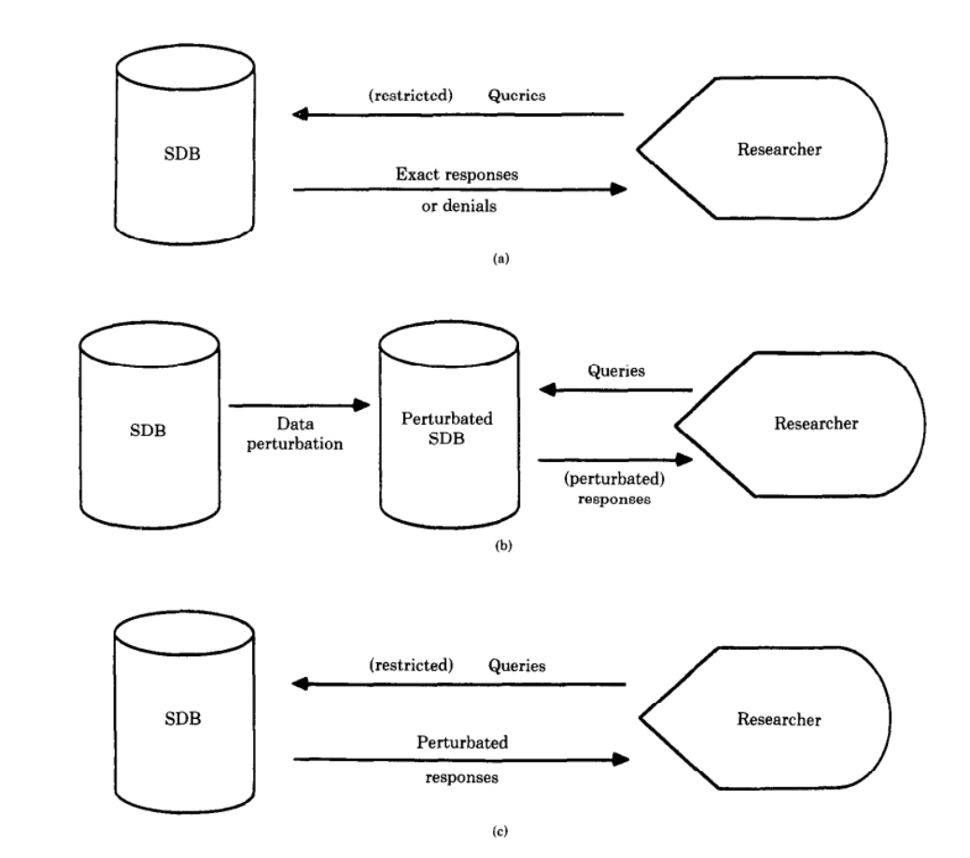
\includegraphics[width=1\linewidth]{assets/text.png}
\caption{Схемы безопасности СБД}
\label{fig:SDB_secure}
\end{figure}

\subsection{Критерии безопасности статистических баз данных}

Критерии безопасности включают оценку вероятности раскрытия записей в СБД, оценку консистентности данных при использовании методов возмущения данных и оценку зависимости между возмущением и конкретными записями. Также учитываются затраты, связанные с выполнением запросов, и назначается конкретная цена каждому запросу. Пользователям предоставляется начальная сумма, которую они могут использовать для запросов, чтобы предотвратить выведение данных.
\\

Когда речь идет о критериях безопасности, необходимо отметить, что полной гарантии безопасности в статистических базах данных (СБД) достичь невозможно. Вместо этого проводится оценка важности деанонимизированных данных и статистической точности, учитывая предпринятые меры по защите данных.
\\

Критерий безопасности "Security" оценивает вероятность раскрытия (включая частичное раскрытие) записи в СБД. Для каждого разрешенного агрегирующего запроса проводится оценка критерия безопасности. Основываясь на количестве информации в базе данных, можно определить, сколько запросов требуется для деанонимизации данных. На основе этой оценки определяется минимальный размер выборки для таких запросов.
\\

Критерий безопасности "Consistency" оценивает консистентность данных для методов возмущения данных. Оценивается степень возмущения данных путем создания агрегирующего запроса и измерения его изменений после внесения возмущений. 
\\

Критерий безопасности "Robustness" оценивает зависимость между возмущением и конкретными записями. Желательно, чтобы возмущение не зависело от данных, однако необходимо сохранить статистические свойства данных.
\\

Критерий безопасности "Costs" определяет конкретную стоимость каждого запроса. Пользователю предоставляется начальная сумма, которую он может использовать для запросов, чтобы предотвратить вывод данных. Этот критерий скорее представляет собой метод управления, а не непосредственный критерий безопасности.
\\

Таким образом, применение критериев безопасности в СБД позволяет оценивать уровень безопасности, учитывая важность данных, статистическую точность, консистентность, робастность и стоимость запросов.
\\

Исходя из вышеизложенных глав, можем убедиться, что безопасность статистических баз данных является сложной задачей, но существуют различные подходы и методы для обеспечения безопасности данных. Каждый подход имеет свои преимущества и недостатки, и выбор методов безопасности должен основываться на анализе конкретных требований и контекста использования СБД. Оценка важности данных, статистической точности и затрат помогает принять решение о применении конкретных методов обеспечения безопасности.



\section{Распознавание вторжений в БД}



\subsection{Основные понятия}

\textbf{Обнаружение вторжений} (применительно к БД) -- процесс выявления действий, 
которые способны нарушить конфиденциальность, целостность и доступность информации, 
хранимой в базе данных (БД).

\textbf{Система обнаружения вторжений} (СОВ) [согласно ФСТЭК] -- программное или 
программно-техническое средство, реализующие функции автоматизированного обнаружения 
(блокирования) действий в информационной системе, направленных на преднамеренный доступ 
к информации, специальные воздействия на информацию (носители информации) в целях ее 
добывания, уничтожения, искажения и блокирования доступа к ней.

Применение систем обнаружения вторжения относится к реактивным мерам (то есть к таким 
мерам, которые используются уже после того, как произошел инцидент) для противодействия 
активности злоумышленника в тех случаях, когда злоумышленник преодолел все проактивные 
меры. Поэтому обычно системы обнаружения вторжений являются \textit{вторичным фактором 
защиты в общей системе защиты} и предназначены для обнаружения и регистрации уже 
произошедних событий, а также оповещение персонала при срабатывании определенных правил.

Если классифицировать методы обнаружения вторжения, используемые в системах обнаружения 
вторжений (СОВ), то можно выделить три типа (согласно классификации, предложенной 
Стефаном Аксельсоном [\cite{IDSClassification}]):
\begin{itemize}
	\item синтаксические методы (или методы поиска злоупотреблений, англ. misuse detection).
		К таким методам обычно относятся методы, которые основываются на обнаружения 
		вторжений путём сравнения SQL-запросов с шаблонами недопустимых синтаксических 
		конструкций.

	\item методы обнаружения аномалий (англ. anomaly detection).
		Такие методы, наоборот, в отличие от первого типа, подрузамевают создание шаблонов 
		нормального поведения пользователя и последующее сравнение этих шаблонов с действиями, 
		выполняемыми пользователями во время работы с БД.

	\item смешанные методы, представляющие собой композицию первых двух
\end{itemize}



\subsection{Системы распознавания вторжений}

Системы обнаружения вторжения (англ. Intrusion Detection System, IDS) и системы 
предотвращения вторжений (англ. Intrusion Preventation System, IPS) обычно рассматриваются 
вместе, причем часто под термином система предотвращение вторжений подрузамевается
расширение систем обнаружения вторжений, так как IPS системы также должны обладать 
возможностью обнаружения вторжений. Иначе говоря, IPS системы являются активными IDS системами.

В IDS системах, система также ответственна за реализацию ответных мер на нарушения: 
блокировка соединения, настройки межсетевого экрана и прочее. Таким образом,

\textbf{Система обнаружения и предотвращения вторжений (IPS/IDS)} (применительно к БД) -- это 
программное или программно-техническое средство, предназначенное для выявления фактов 
неавторизованного доступа и предотвращания попыток несанкционированного доступа к БД.



\subsubsection{Типы моделей систем распознавания вторжений (ID-систем)}

Существует множество способов классификации СОВ, которые не являются однозначными или 
обязательными. Следует рассмотреть наиболее известные и используемые классификации, 
которые характеризуют систему по:
\begin{itemize}
	\item \textbf{По способу мониторинга}
	
	\item \textbf{По способу анализа}
	
	\item \textbf{По скорости реакции}
	
	\item \textbf{По классу защиты}
\end{itemize}


\paragraph*{По способу мониторинга.}

\begin{itemize}
	\item \textbf{Сетевая СОВ (англ. Network-based IDS, NIDS)} -- система, 
	которая занимается проверкой сетевого трафика с концентратора или коммутатора и 
	анализируя сетевые пакеты.

	\item \textbf{Узловая СОВ (англ. Host-based IDS, HIDS)} -- система, 
	отслеживающая вторжения, используя анализ системных вызовов, логов приложений, 
	модификаций файлов (исполняемых, файлов паролей, системных баз данных), состояния 
	хоста и прочих источников. 

	\item \textbf{Основанная на прикладных протоколах СОВ (англ. Application-based IDS, APIDS)} -- 
	система, в которой ведется наблюдение за специализированными прикладными протоколами 
	и анализ соответствующих данных. Например, на веб-сервере с SQL базой данных СОВ будет 
	отслеживать содержимое SQL команд, передаваемых на сервер.

	\item \textbf{Гибридная СОВ} -- система, которая является композицией нескольких видов 
	систем обнаружения вторжений.
\end{itemize}


\paragraph*{По способу анализа.}

О данной классификации уже говорилось ранее. Она строится по методу анализа событий, 
полученных из источника информации, и методу принятия решения, что происходит 
проникновение. Способами анализа являются \textbf{обнаружение злоупотреблений} и 
\textbf{обнаружение аномалий}.


\paragraph*{По скорости реакции.}

Определяют два типа СОВ по времени между получением информации из источника и ее 
анализом и принятием решения. В зависимости от задержки во времени, СОВ разделятся на:
\begin{itemize}
	\item \textbf{с пакетным режимом (англ. interval-based)}. В таких системах реакция 
	происходит через определенные интервалы времени, а информационный поток от точек 
	мониторинга до инструментов анализа не является непрерывным.

	\item \textbf{непрерывные (англ. real-time)}. В таких системах обрабатывается 
	непрерывный поток информации от источников. При этом таких тип является преобладающей 
	типом в сетевых СОВ, которые получают информацию из потока сетевого трафика.
\end{itemize}


\paragraph*{По классу защиты.}

Для каждой сертифицированной в России СОВ присваивается некоторый класс защиты 
согласно классификации ФСТЭК и выполненным требованиям для определенного профиля защиты (ПЗ).
Всего существует 6 классов, где самый низкий класс - шестой, а самый высокий - первый.

Согласно ФСТЭК СОВ разделяются на [\cite{IDSFSTEK}]:
\begin{itemize}
	\item \textbf{СОВ с 6 классом защиты}: применяются в информационных системах 
	персональных данных 3 и 4 классов.

	\item \textbf{СОВ с 5 классом защиты}: применяются в информационных системах 
	персональных данных 2 класса.

	\item \textbf{СОВ с 4 классом защиты}: применяются в государственных информационных 
	системах, в которых обрабатывается информация ограниченного доступа, не содержащая 
	сведения, составляющие государственную тайну, в информационных системах персональных 
	данных 1 класса, а также в информационных системах общего пользования II класса.

	\item \textbf{СОВ с 3, 2 или 1 классом защиты}: применяются в информационных системах, 
	в которых обрабатывается информация, содержащая сведения, составляющие государственную 
	тайну.
\end{itemize}



\subsubsection{Общая структура ID-систем} 


\paragraph*{Архитектура СОВ.} Основнымы архитектурными компонентами СОВ являются: 

\begin{enumerate}
	\item \textbf{Host} -- система, на которой выполняется ПО СОВ.
	
	\item \textbf{Target} -- система, за которой наблюдает СОВ.
\end{enumerate}

Первоначально многие СОВ выполнялись на тех же системах, которые они защищали. 
Основная причина этого была в том, что большинство систем было mainframe, и стоимость 
выполнения СОВ на отдельном компьютере была очень большой. Это создавало проблему с 
точки зрения безопасности, так как любой атакующий, который успешно атаковал целевую 
систему, мог в качестве одной из компонент атаки просто запретить функционирование СОВ.

Но с появлением рабочих станций и персональных компьютеров в большинстве архитектур 
СОВ предполагается выполнение СОВ на отдельной системе, тем самым разделяя системы 
Host и Target. Это улучшает безопасность функционирования СОВ, так как в этом случае 
проще спрятать существование СОВ от атакующих.


\paragraph*{Компоненты современных СОВ:}

\begin{itemize}
	\item сенсор, который отслеживает события в сети или системе;
	
	\item анализатор событий, обнаруженных сенсорами;
	
	\item компонента принятия решения.
\end{itemize}


\paragraph*{Способы управления СОВ:}

\begin{itemize}
	\item \textbf{Централизованное управление}. При централизованных стратегиях управления 
	весь мониторинг, обнаружение и отчетность управляются непосредственно с единого "поста". 
	В этом случае существует единственная консоль СОВ, которая связана со всеми сенсорами, 
	расположенными в сети.

	\item \textbf{Частично распределенное управление}. Мониторинг и определение управляются 
	с локально управляемого узла, с иерархической отчетностью в одно или более центральных 
	расположений.

	\item \textbf{Полностью распределенное управление}. Мониторинг и определение выполняются 
	с использованием подхода, основанного на агентах, когда решения об ответе делаются в 
	точке анализа.
\end{itemize}

При этом в сети должны поддерживаться следующие связи:

\begin{itemize}
	\item связи для передачи отчетов СОВ. Эти связи создаются между сенсорами как сетевого 
	мониторинга, так и мониторинга хоста, и центральной консолью СОВ;

	\item связи для мониторинга хостов и сетей;
	
	\item связи для выполнения ответов СОВ.
\end{itemize}



\subsubsection{Шаблоны классов пользователей}

Рассматривать шаблоны классов пользователей имеет смысл только в контексте СОВ, 
применяющих методы обнаружения аномалий, так как именно они строят и используют 
такие шаблоны поведения пользователей. Таким образом, детекторы аномалий определяют 
необычное поведение на хосте или в сети. Они предполагают, что атаки отличаются от 
некоторой нормальной деятельности и могут, следовательно, быть определены системой, 
которая умеет отслеживать эти отличия. Детекторы аномалий создают профили, представляющие 
собой нормальное поведение пользователей, хостов или сетевых соединений. Эти профили 
создаются, исходя из данных истории, собранных в период нормального функционирования. 
Затем детекторы собирают данные о событиях и используют различные метрики для определения 
того, что анализируемая деятельность отклоняется от нормальной.

Метрики и технологии, используемые при определении аномалий, включают:

\begin{itemize}
	\item определение допустимого порога. В этом случае основные атрибуты поведения 
	пользователя и системы выражаются в количественных терминах. Для каждого атрибута 
	определяется некоторый уровень, который устанавливается как допустимый. Такие атрибуты 
	поведения могут определять число файлов, доступных пользователю в данный период времени, 
	число неудачных попыток входа в систему, количество времени ЦП, используемое процессом и 
	т.п. Данный уровень может быть статическим или эвристическим — например, может определяться 
	изменением анализируемых значений.

	\item статистические метрики: параметрические, при которых предполагается, что распределение 
	атрибутов профиля соответствует конкретному образцу, и непараметрические, при которых 
	распределение атрибутов профиля является "обучаемым" исходя из набора значений истории, 
	которые наблюдались за определенный период времени.

	\item метрики, основанные на правилах, которые аналогичны непараметрическим статистическим 
	метрикам в том, что наблюдаемые данные определяют допустимые используемые образцы, но 
	отличаются от них в том, что эти образцы специфицированы как правила, а не как численные 
	характеристики.

	\item другие метрики, включая нейросети, генетические алгоритмы и модели иммунных систем.
\end{itemize}


\paragraph*{Преимущества определения аномалий:}

\begin{itemize}
	\item IDS, основанные на определении аномалий, обнаруживают неожиданное поведение и, 
	таким образом, имеют возможность определить симптомы атак без знания конкретных деталей атаки.

	\item Детекторы аномалий могут создавать информацию, которая в дальнейшем будет 
	использоваться для определения сигнатур для детекторов злоупотреблений.
\end{itemize}


\paragraph*{Недостатки определения аномалий:}

\begin{itemize}
	\item Подходы определения аномалий обычно создают большое количество ложных сигналов 
	при непредсказуемом поведении пользователей и непредсказуемой сетевой активности.

	\item Подходы определения аномалий часто требуют некоторого этапа обучения системы, 
	во время которого определяются характеристики нормального поведения.
\end{itemize}



\subsubsection{Модели известных атак}

Далее будут рассмотрены основные типы SQL-инъекций \autocite{proglib} Рассмотрены они будут на простом примере критически уязвимой страницы
\begin{figure}[h]
    \centering
    \includegraphics[width=0.8\textwidth]{assets/sql_ijection_example.png}
    \caption{Пример уязвимой страницы}
    \label{fig:mesh1}
\end{figure}

\begin{itemize}
    \item \textbf{Атаки комментированием}\\
    Использование однострочных комментариев позволяет игнорировать часть запроса, идущую после вашей инъекции. Например, ввод в уязвимое поле Username запроса admin'-- позволит зайти на ресурс под администратором, потому что поверка пароля будет закомментирована.\\
    \begin{grayquote} 
        SELECT * FROM members WHERE username = 'admin'--' AND password = 'password'
    \end{grayquote}
    
    Многострочные комментарии могут справится с проверкой или определить тип базы данных.
    Например, подобные запросы обойдут примитивный текстовый анализ:\\
    \begin{grayquote} 
        DROP/*some comment*/sampletable\\
        DR/**/OP/*random comment to cheat*/sampletable
    \end{grayquote}
    
    \item \textbf{Манипуляции со строками}\\
    При помощи конкатенации строк можно обходить фильтр кавычек.\\
    \begin{grayquote} 
        SELECT CONCAT(login, password) FROM members
    \end{grayquote}

    Можно представлять строки в шеснадцатиричном виде, с помощью функции HEX() или вводить их посимвольно.
    \begin{grayquote}
        //0x633A5C626F6F742E696E69 == c:\textbackslash boot.ini\\
        SELECT CONCAT('0x','633A5C626F6F742E696E69'))\\
        SELECT CONCAT(CHAR(75),CHAR(76),CHAR(77))
    \end{grayquote}
    
    \item \textbf{Обход аутентификации}\\
    При помощи OR и сравнения констант можно обойти форму аутентификации. Существуют даже словари, содержащие основные запросы для обхода уязвимой формы

    Примеры запросов:\\
    \begin{grayquote} 
        ' or 1=1\\
        ' or 1=1--\\
        ' or 1=1\#\\
        admin' --\\
        admin' or '1'='1
    \end{grayquote}
    
    \item \textbf{Union injection}\\
    При помощи UNION комбинировать данные из разных таблиц в одну. Это одна из самых популярных и опасных классических инъекций.

    Допустим, на сайте есть список товаров с уязвимой строкой поиска. Тогда, подобрав правильное количество колонок и определив их название, через UNION можно вывести практически любые данные
    \begin{grayquote} 
        SELECT name, price FROM products UNION ALL SELECT name, pass FROM members\\
        \#Такой запрос позволит получить данные о таблицах и найти таблицу пользователей\\
        UNION(SELECT TABLE\_NAME, 

        TABLE\_SCHEMA FROM information\_schema.tables)
    \end{grayquote}
    
    \item \textbf{Последовательные запросы}\\
    В некоторых СУБД можно использовать простой знак ';' для последовательного вызова вредоносных запросов
    \begin{grayquote} 
        \#Удаление таблицы\\
        SELECT * FROM products WHERE productName = ""; DROP users--\\
        \#Выключение SQL Server\\
        SELECT * FROM products WHERE productName = ""; shutdown –\\
    \end{grayquote}


    \item \textbf{Error-based injection}\\
    Инъекции, основанные на том, что злоумышленник может видеть вывод ошибки. Уязвимость устраняется просто отключением этого вывода

    Последовательное выполнение следующих запросов может помочь определить в тексте ошибки названия столбцов:\\
    \begin{grayquote} 
        ' HAVING 1=1 --\\
        ' GROUP BY table.columnfromerror1 HAVING 1=1 --\\
        ' GROUP BY table.columnfromerror1, columnfromerror2 HAVING 1=1 --\\
        .....\\
        ' GROUP BY table.columnfromerror1, columnfromerror2, columnfromerror(n) HAVING 1=1 --\\
        Если ошибки перестали появляться, значит столбцы закончились
    \end{grayquote}
    
    
    \item \textbf{Error-based injection}\\
    Инъекции, основанные на том, что злоумышленник может видеть вывод ошибки. Уязвимость устраняется просто отключением этого вывода

    Последовательное выполнение следующих запросов может помочь определить в тексте ошибки названия столбцов:\\
    \begin{grayquote} 
        ' HAVING 1=1 --\\
        ' GROUP BY table.columnfromerror1 HAVING 1=1 --\\
        ' GROUP BY table.columnfromerror1, columnfromerror2 HAVING 1=1 --\\
        .....\\
        ' GROUP BY table.columnfromerror1, columnfromerror2, columnfromerror(n) HAVING 1=1 --\\
        Если ошибки перестали появляться, значит столбцы закончились
    \end{grayquote}
    
    \item \textbf{Boolean-based blind injection}\\
    Если атакующий все же может получить информацию о наличии или отсутствии ошибки из HTTP-статуса, в сервисе имеется уязвимость к обычной слепой атаке. Рассмотрим запрос, который позволит нам при помощи алгоритма бинарного поиска посимвольно определить название первой таблицы и в дальнейшем всех данных
    
    \begin{grayquote} 
        TRUE : SELECT ID, Username, Email FROM [User]WHERE ID = 1 AND \\
        ISNULL(ASCII(SUBSTRING((SELECT TOP 1 name FROM sysObjects WHERE xtYpe=0x55 AND\\ 
        name NOT IN(SELECT TOP 0 name FROM sysObjects WHERE xtYpe=0x55)),1,1)),0)>78--\\
        \#Этот запрос говорит нам, что ASCII-значение первого символа больше 78 \\
        \#дальнейший перебор определит точное значение 
    \end{grayquote}
    
    \item \textbf{Time-based blind injection}\\
    Если атакующий не наблюдает никаких отличий в ответах сервера, можно попробовать SLEEP или WAIT FOR DALAY
    
    \begin{grayquote} 
        SELECT * FROM products WHERE id=1; WAIT FOR DELAY '00:00:15'
    \end{grayquote}
    Конечно, реальные примеры будут выглядеть примерно как boolean-based, только true и false атакующий будет отличать по времени отклика
\end{itemize}



\subsection{Экспертные ID-системы}

Технологию построения экспертных систем часто называют инженерией имплекационных правил. Как правило, 
этот процесс требует специфической формы взаимодействия создателя имплекационных правил и одного 
или нескольких экспертов в некоторой предметной области. Инженер имплекационных правил <<встраивает>>
процедуры, стратегии, эмпирические правила в экспертную систему. В результате появляется 
компьютерная программа, которая решает задачи во многом так же, как эксперты -- люди.
\autocite{BeynonDavies}

Главное преимущество использования продукционных систем заключается в возможности разделения причин и 
решений возникающих проблем.

В экспертных системах могут использоваться импликационные правила (\textbf{Если} \textit{условие} то 
\textbf{действие}).

Например:
\begin{itemize}
	\item ЕСЛИ с одного узла за время T поступает N пакетов, ТО записать в лог факт: 
	происходит DoS атака (факт А)
	
	\item Если наблюдается более чем N фактов А, ТО записать в лог факт: происходит DDoS атака
\end{itemize}

Основные проблемы, которые обычно возникают при их практическом применении:
\begin{itemize}
    \item Недостаточная эффективность при работе с большими объемами данных.
    \item Трудно учесть зависимую природу данных параметров оценки.
\end{itemize}

При использовании продукционных систем для обнаружения вторжений можно установить символическое 
проявление вторжения при помощи имеющихся данных.

\textbf{Существует 3 вида Expert System}, отличаются они по методу 
получения имплекационных 
правил\autocite{IDSystem}:

\begin{itemize}
	\item Статистическая модель - эксперт сам задает веса параметров в общей функции анамальности.
	\item Нейросетевая модель - веса параметров задаются за счет обучения нейросетевой модели 
	(эксперт задает архитектуру модели и обучающую выборку).
	\item Генерация патернов - эксперт задает связи (правила) между событиями безопасности.
\end{itemize}

\textbf{Трудности:}
\begin{itemize}
    \item Отсутствие встроенной или естественной обработки порядка последовательностей в анализируемых 
    данных. База фактов, соответствующая левой части «продукции», используется для определения правой 
    части. В левой части продукционного правила все элементы объединяются при помощи связи «и».
    \item Встроенная экспертиза хороша только в том случае, если моделируемые навыки администратора 
    безопасности не противоречивы. Это практическое рассуждение, возможно, касается 
    недостаточной централизованности усилий экспертов безопасности в направлении создания 
    исчерпывающих множеств правил. Обнаруживаются только известные уязвимости.
    \item Существуют определенный программный инжиниринг, связанный с установкой (поддержанием) баз знаний. 
    При добавлении или удалении какого-либо из правил должно изменяться остальное множество правил.
    \item Обнаруживаются только известные уязвимости.
    \item Объединение различных измерений вторжений и создание связанной картины вторжения приводит к 
    тому, что частные причины становятся неопределенными. Ограничения продукционных систем, в 
    которых используется неопределенная причина, довольно хорошо известны.
\end{itemize}
\autocite{BeynonDavies}



\subsubsection{Метрики}

\begin{itemize}
	\item \textbf{Показатель активности} -- величина, при превышении которой активность 
	подсистемы оценивается как быстро прогрессирующая. В общем случае используется для 
	обнаружения аномалий, связанных с резким ускорением в работе. Пример: среднее число 
	записей аудита, обрабатываемых для элемента защищаемой системы в единицу времени.

	\item \textbf{Распределение активности в записях аудита} -- распределение во всех типах 
	активности в актуальных записях аудита. Здесь под активностью понимается любое действие 
	в системе, например, доступ к файлам, операции ввода-вывода.

	\item \textbf{Измерение категорий} -- распределение определенной активности в 
	категории \footnotemark. Например, относительная частота количества регистраций в 
	системе (логинов) из каждого физического места нахождения. Предпочтения в использовании 
	программного обеспечения системы (почтовые службы, компиляторы, командные интерпретаторы, 
	редакторы и т.д.)

	\item \textbf{Порядковые измерения} -- используется для оценки активности, поступающей 
	в виде цифровых значений. Например, количество операция ввода-вывода, инициируемых каждым 
	пользователем. Порядковые изменения вычисляют общую числовую статистику значений определенной 
	активности, в то время как измерение категорий подсчитывает количество активностей.
\end{itemize}
\autocite{BeynonDavies}
\footnotetext{Здесь под \textit{категорией} понимается группа подсистем, объединенных по 
некоему общему принципу}



\subsubsection{Статистические модели}

При обнаружении аномалий с использованием профайла в основном применяют статистические 
методы оценки. Процесс обнаружения происходит следующим образом: текущие значения измерений 
профайла сравнивают с сохраненными значениями. Результат сравнения - показатель аномальности 
в измерении. Общий показатель аномальности в простейшем случае может вычисляться при помощи 
некоторой общей функции от значений показателя аномалии в каждом измерении профайла.

Например, пусть $M_1, M_2, \dots, M_n$ -- измерения профайла, а $S_1, S_2, \dots, S_n$ -- 
соответственно представляют собой значения аномалии каждого из измерений. Чем больше 
число $S_i$, тем больше аномалии в $i$-ом показателе. Объединяющая функция может быть 
взвешенной суммой их квадратов:

\begin{equation}
	a_1s_1^2 + a_2s_2^2 + \dots + a_ns_n^2 > 0,
\end{equation}

где $a_i$ -- отражает относительный вес метрики $M_i$.

Параметры $M_1, M_2, \dots, M_n$ могут быть зависимыми друг от друга. В таком случае, 
объединяющая функция будет более сложной.\autocite{IDSystem}

\textbf{Основное преимущество} заключается в том, что применяются хорошо известные статистические методы.

\textbf{Недостатки:}
\begin{itemize}
	\item Нечувствительность к последовательности возникновения событий. 
	То есть статистическое обнаружение может упустить вторжение, 
	которое проявляется в виде последовательности сходных событий.
	
	\item Система может быть последовательно обучена таким образом, что аномальное поведение 
	будет считаться нормальным. Злоумышленники, которые знают, что за ними наблюдают 
	при помощи таких систем, могут обучить их для использования в своих целях. Именно поэтому в 
	большинстве существующих схем обнаружения вторжения используется комбинация подсистем 
	обнаружения аномалий и злоупотреблений.

	\item Трудно определить порог, выше которого аномалии можно рассматривать как вторжение. 
	Занижение порога приводит к ложному срабатыванию (false positive), а завышение – к пропуску вторжений (false negative).

	\item Существуют ограничения к типам поведения, которые могут быть смоделированы, 
	используя чистые статистические методы. Применение статистических технологий для 
	обнаружения аномалий требует предположения, что данные поступают от квазистатического процесса.
\end{itemize}
\autocite{IntrusionDetection}


\subsubsection{Профили}

Одним из способов формирования <<образа>> нормального поведения системы состоит в 
накоплении измерений значения параметров оценки в специальной структуре данных. 
Эта структура данных называется \textit{профайлом}.\autocite{IDSystem} 

Основные требования, предъявляемые к структуре профайла:
\begin{itemize}
	\item Минимальный конечный размер
	
	\item Быстрое выполнение операции обновления
\end{itemize}



\subsubsection{Нейронные сети для представления профиля}
Другой способов представления «образа» нормального поведения системы – обучение нейронной 
сети значениями параметров оценки.

Обучение нейронной сети осуществляется последовательностью информационных единиц (далее команд), 
каждая из которых может находиться на более абстрактном уровне по сравнению с используемыми 
параметрами оценки. Входные данные сети состоят из текущих команд и прошлых \textbf{W} команд, которые 
обрабатываются нейронной сетью с целью предсказания последующих команд; \textbf{W} также называют размером
окна. После того как нейронная сеть обучена множеством последовательных команд защищаемой системы или 
одной из ее подсистем, сеть представляет собой «образ» нормального поведения. Процесс обнаружения 
аномалий представляет собой определение показателя неправильно предсказанных команд, 
то есть фактически обнаруживается отличие в поведение объекта. На уровне рецептора стрелки 
показывают входные данные последних \textbf{W} команд, выполненных пользователем. Входной параметр задает 
несколько значений или уровней, каждый из которых уникально определяет команду. Выходной реагирующий 
слой состоит из одного многоуровневого, который предсказывает следующую возможную команду пользователя.
\autocite{BeynonDavies}

\begin{figure}[h!]
    \centering
    \includegraphics[width=0.8\textwidth]{assets/intrusion/нейронные сети.jpg}
\end{figure}

\textbf{Недостатки:}
\begin{itemize}
    \item Топология сети и веса узлов определяются только после огромного числа проб и ошибок.
    \item Размер окна – еще одна величина, которая имеет огромное значение при разработке. 
    Если сделать окно маленьким то сеть будет не достаточно производительной, слишком большим 
    – будет страдать от неуместных данных.
\end{itemize}

\textbf{Преимущества:}
\begin{itemize}
    \item Успех данного подхода не зависит от природы исходных данных.
    \item Нейронные сети легко справляются с зашумленными данными.
    \item Автоматически учитываются связи между различными измерениями, которые, 
    несомненно, влияют на результат оценки.
\end{itemize}
\autocite{BeynonDavies}


\subsubsection{Генерация патернов}
Представление «образа» в данном случае основывается на предположении о том, что текущие значения 
параметров оценки можно связать с текущим состоянием системы. После этого функционирование 
представляется в виде последовательности событий или состояний.

Были предложены временные правила, которые характеризуют совокупности значений параметров оценки 
(далее паттерна) нормальной (не аномальной) работы. Эти правила формируются индуктивно и заменяются 
более «хорошими» правилами динамически во время обучения. Под «хорошими правилами» понимаются правила 
с большей вероятностью их появления и с большим уровнем уникальности для защищаемой системы. 
Для примера рассмотрим следующее правило:

\begin{equation}
	E1 \rightarrow E2\rightarrow E3 \Rightarrow E4 = 0.95, E5 = 0.05
\end{equation}
где Е1\dotsЕ5 - события безопасности.

Это утверждение, основанное на ранее наблюдавшихся данных, говорит о том, что для последовательности 
паттернов установилась следующая зависимость: если имеет место \textbf{Е1} и далее \textbf{Е2} и \textbf{Е3},
то после этого вероятность проявления \textbf{Е4} - 0.95 и \textbf{Е5} – 0.05.

Именно множество правил, создаваемых индуктивно во время наблюдения работы пользователя, составляет «образ». 
Аномалия регистрируется в том случае, если наблюдаемая последовательность событий соответствует левой 
части правила выведенного ранее, а события, которые имели место в системе после этого, 
значительно отличаются от тех, которые должны были наступить по правилу.

\textbf{Основной недостаток} данного подхода заключается в том, что неузнаваемые паттерны поведения могут 
быть не приняты за аномальные из-за того, что они не соответствуют ни одной из левых частей 
всех правил.\autocite{IDSystem}

Данный метод довольно эффективно определяет вторжения, так как принимаются во внимание:
\begin{itemize}
    \item Зависимости между событиями.
    \item Последовательность появления событий.
\end{itemize}

\textbf{Достоинства метода:}
\begin{itemize}
    \item Лучшая обработка пользователей с большим колебанием поведения, но с четкой 
    последовательностью паттернов.
    \item Возможность обратить внимание на некоторые важные события безопасности, а не на всю сессию, 
    которая помечена как подозрительная.
    \item Лучшая чувствительность к обнаружению нарушений: правила содержат в себе семантику процессов, что позволяет гораздо проще заметить злоумышленников, которые пытаются обучить систему в своих целях.
\end{itemize}
\autocite{IntrusionDetection}

\subsubsection{Примеры ID-систем}


\paragraph*{GreenSQL} (APIDS система) -- межсетевой экран, функционирующий как 
прокси-сервер между веб-приложением и SQL сервером. То есть приложение устанавливает 
соединения к БД не напрямую, а через сервер GreenSQL. GreenSQL анализирует SQL запросы 
на предмет аномальных запросов, и в случае нормального запроса (то есть если степень 
риска запроса мала) перенаправляет его на внутренний сервер БД.

GreenSQL поддерживает следующие режимы работы:
\begin{itemize}
	\item \textbf{Режим симуляции (англ. Simulation Mode)} -- пассивная система обнаружения 
	атак (IDS). Протоколирует SQL запросы, выдает предупреждения на консоль управления.

	\item \textbf{Блокировка подозрительных команд (англ. Blocking Suspicious Commands/Risk Based)} -- 
	активная СОВ. Атаки не только обнаруживаются, но и блокируются (IPS) в соответствии с 
	установленными правилами, указывающими на аномальность запроса.

	\item \textbf{Активная защита от неизвестных запросов (англ. Database Firewall)} -- 
	блокирование всех неизвестных запросов.

	\item \textbf{Режим обучения (англ. Learning mode)} -- предназначен для прогона и 
	настройки правил в <<чистой>> среде, что позволяет сформировать белый список и 
	предотвратить в последствии ложные срабатывания анализатора запросов.
\end{itemize}

Особенности GreenSQL:
\begin{itemize}
	\item Поддержка ряда СУБД: Microsoft SQL 2000/2005/2008, MySQL 4.x/5.x, PostgreSQL 7.x/8.x. 
	
	\item Является кросс-платформенной. Среди официально поддерживаемых платформ Microsoft 
	Windows Server 2003/2008, Ubuntu, CentOS. Поддерживаются 32-х и 64-х разрядные системы.

	\item GreenSQL находит подозрительные запросы, используя ряд методов: 
	\begin{itemize}
		\item Путем определения административных и чувствительных команд SQL. 
		Например: SHOW TABLES, CREATE TABLE, ALTER TABLE.

		\item Путем подсчета риска запроса. На это может влиять пустая строка пароля, "or" 
		внутри запроса или выражения SQL, которые всегда возвращают истину (1=1).
	\end{itemize}

\end{itemize}


\paragraph*{Snort} (NIDS система) -- свободная сетевая система предотвращения вторжений (IPS) 
и обнаружения вторжений (IDS) с открытым исходным кодом, способная выполнять регистрацию 
пакетов и в реальном времени осуществлять анализ трафика в IP-сетях. 

Snort поддерживает следующие режимы работы:
\begin{itemize}
	\item \textbf{Sniffer mode}. В таком режиме программа только считывает сетевые пакеты и 
	выводит их на консоль. 

	\item \textbf{Packet Logger Mode}. В режиме логирования пакетов, программа будет 
	регистрировать/логировать пакеты на диске.

	\item \textbf{Network Intrusion Detection System Mode}. В режиме обнаружения вторжений 
	программа будет отслеживать сетевой трафик и анализировать его в соответствии с набором 
	правил, определенным пользователем. Затем программа выполнит определенное действие, 
	основанное на том, что было идентифицировано.
\end{itemize}

Особенности Snort:
\begin{itemize}
	\item Возможность написания собственных правил.
	\item Расширение функциональности с помощью подключения дополнительных модулей.
	\item Гибкая система оповещения об атаках: Log-файлы, устройства вывода, БД и прочие.
\end{itemize}


\paragraph*{Suricata} (NIDS система) -- свободная сетевая система предотвращения вторжений 
(IPS) и обнаружения вторжений (IDS) с открытым исходным кодом. Основана разработчиками, 
которые трудились над IPS версией Snort, поэтому имеет схожий функционал и обладает полной 
поддержкой формата правил Snort.

Особенности Suricata:
\begin{itemize}
	\item Многозадачность.
	
	\item Автоматическое определение протокола.
	
	\item Высокая производительность, позволяющая обрабатывать трафик до 10Gbit на обычном 
	оборудовании.
\end{itemize}


\paragraph*{Sagan} (HIDS система) -- многопоточная, высокопроизводительная система 
анализа журналов и мониторинга появления в логах событий, связанных с безопасностью, 
и реагирования на эти события в режиме реального времени. Система работает в операционных 
системах Unix. 

Sagan также относится к категории систем управления инцидентами и событиями информационной 
безопасности (англ. Security Information and Log Management, SEIM).



\subsection{Развитие систем распознавания вторжений}

\subsubsection{Развитие практических аспектов СОВ}

Коммерческое использование СОВ находится в стадии формирования. Некоторые коммерческие 
СОВ получили негативную публичную оценку за большое число ложных срабатываний, неудобные 
интерфейсы управления и получения отчетов, огромное количество отчетов об атаках, 
плохое масштабирование и плохую интеграцию с системами сетевого управления. Тем не менее 
потребность в хороших СОВ возрастает, поэтому с большой вероятностью эти проблемы будут 
успешно решаться в ближайшее время.

Ожидается, что улучшение качества функционирования СОВ будет осуществляться аналогично 
антивирусному ПО. Раннее антивирусное ПО создавало большое число ложных тревог при 
нормальных действиях пользователя и не определяло все известные вирусы. Однако сейчас 
положение существенно улучшилось, антивирусное ПО стало прозрачным для пользователей 
и достаточно эффективным.

Более того – очень вероятно, что основные возможности СОВ скоро станут ключевыми в 
сетевой инфраструктуре (такой как роутеры, мосты и коммутаторы) и в операционных системах. 
При этом, скорее всего, разработчики СОВ сфокусируют свое внимание на решении проблем, 
связанных с масштабируемостью и управляемостью СОВ.

Имеются также и другие тенденции, которые, скорее всего, будут влиять на функциональности 
СОВ следующего поколения. Существует заметное движение в сторону аппаратно-программных 
(appliance) решений для СОВ. Также вероятно, что в будущем некоторые функции определения 
соответствия шаблону могут быть реализованы в аппаратуре, что увеличит скорость обработки.

Наконец, механизмы, связанные с управлением рисками в области сетевой безопасности, 
будут оказывать влияние на требования к СОВ.



\subsubsection{Развитие теоретических аспектов СОВ}

Дальнейшие направления совершенствования связаны с внедрением в теорию и практику СОВ 
общей теории систем, методов синтеза и анализа информационных систем, конкретного аппарата 
теории распознавания образов. Эти разделы теории предполагают получение конкретных методов 
исследования для области систем СОВ.

До настоящего времени не описана СОВ как подсистема информационной системы в терминах 
общей теории систем. Необходимо обосновать показатель качества СОВ, элементный состав 
СОВ, ее структуру и взаимосвязи с информационной системой.

В связи с наличием значительного количества факторов различной природы, слаженная работа 
информационной системы и СОВ имеет вероятностный характер. Вследствие этого актуальным 
является обоснование вида вероятностных законов конкретных параметров функционирования. 
Особо следует выделить задачу обоснования функции потерь информационной системы, задаваемую 
в соответствии с ее целевой функцией на области параметров функционирования системы. 
При этом целевая функция должна быть определена не только на экспертном уровне, но и в 
соответствии с совокупностью параметров функционирования всей информационной системы и 
задачами, возложенными на нее. В таком случае показатель качества СОВ будет определяться 
как один из параметров, влияющих на целевую функцию, а его допустимые значения -- 
допустимыми значениями функции потерь.

После обоснования законов и функций, реальной задачей является получение оптимальной 
структуры СОВ в виде совокупности математических операций с помощью формализованных 
методов. Таким образом, может быть решена задача синтеза структуры СОВ. На основе 
полученных математических операций можно будет рассчитать зависимости показателей 
качества функционирования СОВ от параметров ее функционирования, а также от параметров 
функционирования информационной системы, то есть, будет возможен реальный анализ качества 
функционирования СОВ.

Сложность применения формализованного аппарата анализа и синтеза информационных систем 
к СОВ заключается в том, что конкретные реализации информационного комплекса и его 
подсистемы - СОВ состоят из разнородных элементов, которые могут описываться различными 
разделами теории (системами массового обслуживания, конечными автоматами, теорией 
вероятности, теорией распознавания образов и т.д.), то есть, рассматриваемый объект 
исследования является составным. В результате, математические модели, по-видимому, 
можно получить только для отдельных составных частей СОВ, что затрудняет анализ и 
синтез СОВ в целом. Однако, дальнейшая конкретизация применения формализованного 
аппарата анализа и синтеза позволит оптимизировать СОВ.

На основе изложенного можно сделать вывод о наличии в практической среде значительного опыта 
решения проблем обнаружения вторжений. Применяемые СОВ в значительной степени основаны на 
эмпирических схемах процесса обнаружения вторжений. Дальнейшее совершенствование СОВ связано 
с конкретизацией методов синтеза и анализа сложных систем, теории распознавания образов в 
применении к СОВ.
\input{part/security}
% \input{part/ref}
\printbibliography
\end{document}
